
\chapter{Rectas y planos}
	
\begin{myblock}

	\begin{figure}[H]
		\centering
		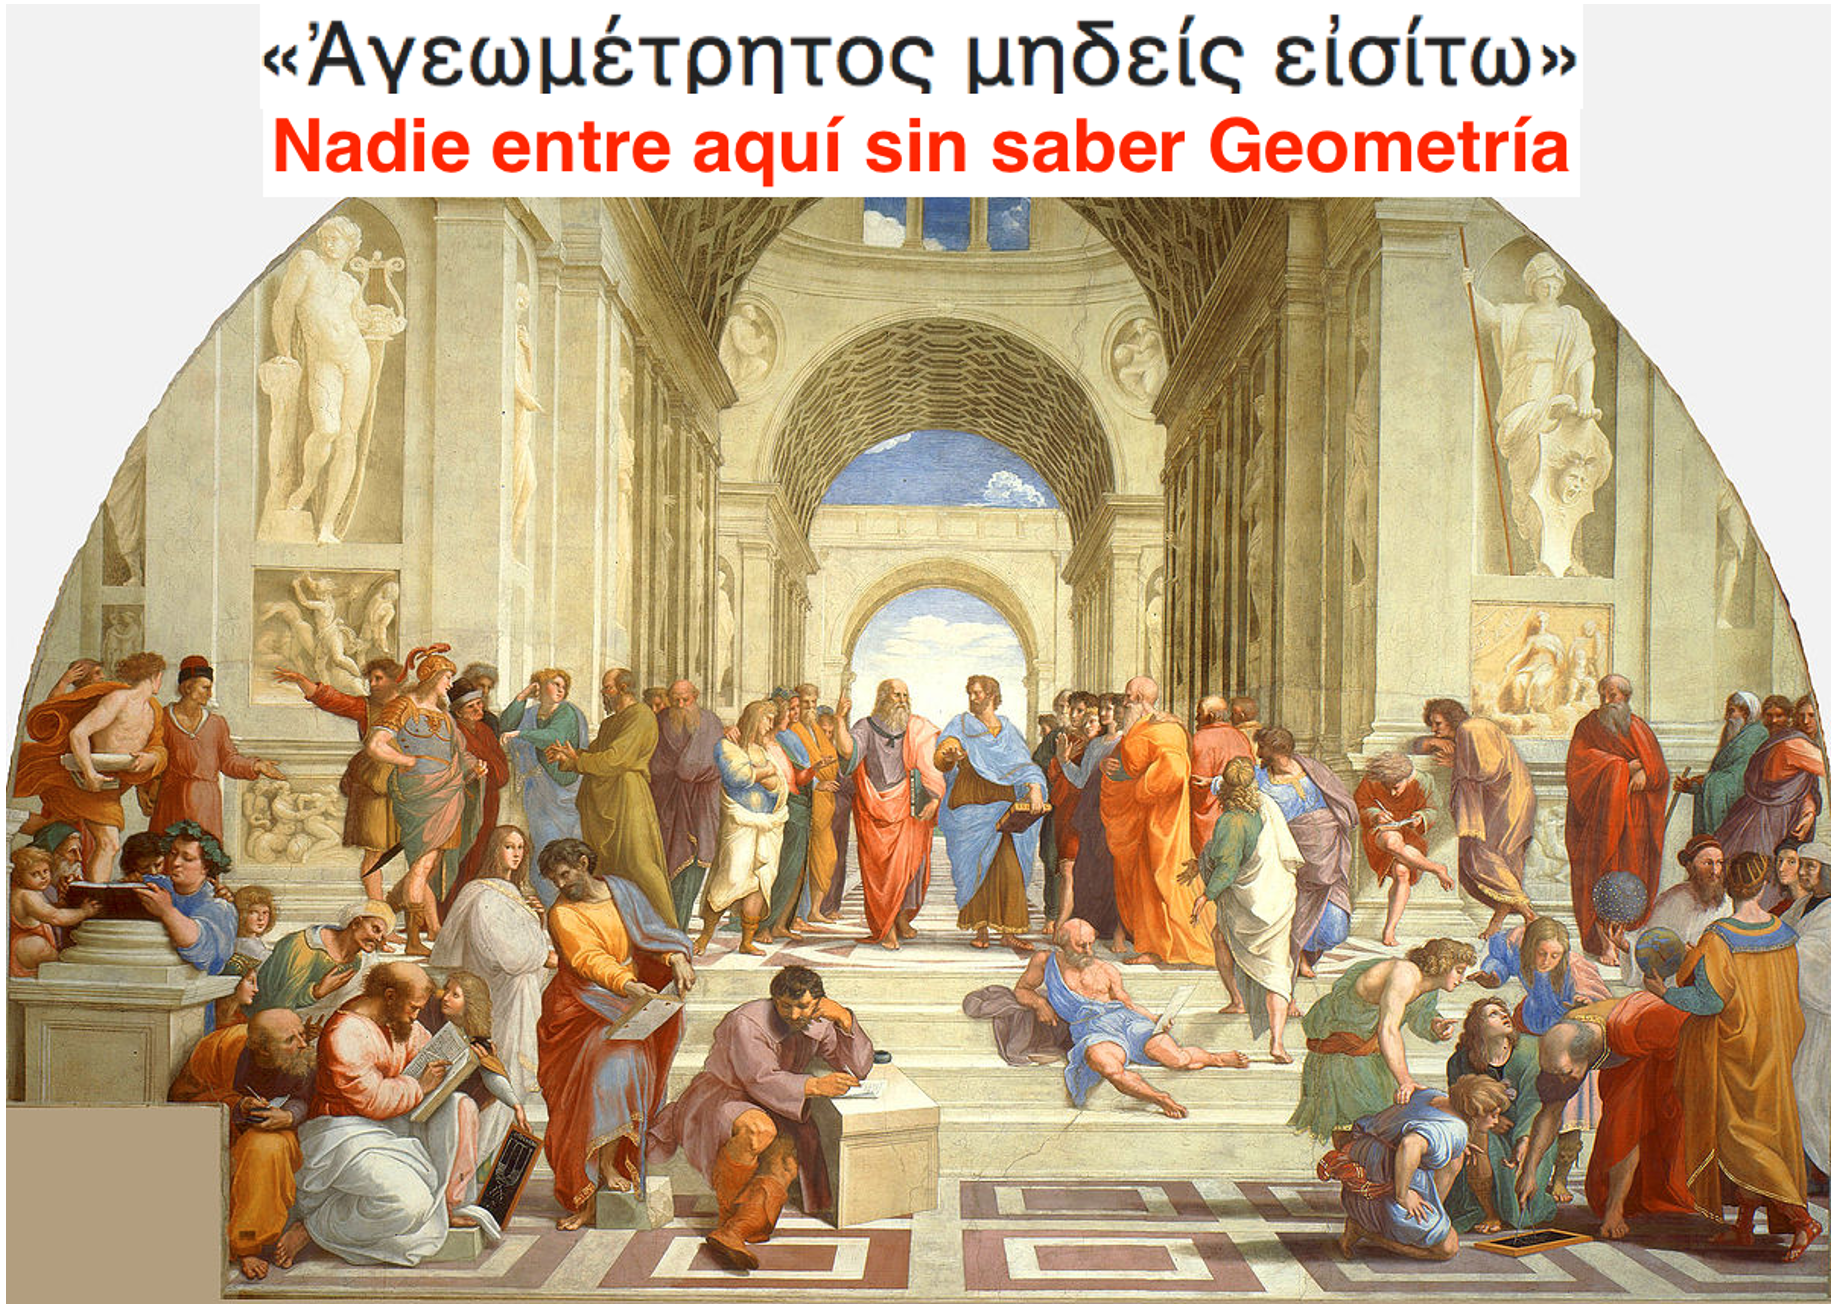
\includegraphics[width=1\textwidth]{imagenes/imagenes10/academia-platon.png}
		\caption*{Inscripción en la Academia de Platón}
	\end{figure}
\end{myblock}

\begin{myexampleblock}{Espacio afín euclídeo}
 
El espacio afín euclídeo es la terna $(E_3 ,(V_3 ,\cdot) ,+)$; `$\; \cdot \; $'  es el producto escalar (la métrica del espacio) y `$\; + \; $' es la ley de Chasles (los vectores desplazan puntos: $A+\vec v = B$)

\vspace{4mm}\textbf{Propiedades afines} (en este tema)

\vspace{2mm}Son propiedades afines todas aquellas que se derivan de la estructura vectorial de $V_3$ , tales como: 

\vspace{2mm}--- Incidencia $\quad$ --- Paralelismo $\quad$ --- Intersección  

\vspace{4mm}\textbf{Propiedades euclídeas} (próximo tema)

\vspace{2mm}Son propiedades euclídeas todas aquellas que se derivan de la estructura métrica de $V_3$ , tales como: 

\vspace{2mm}--- Distancias $\quad$ --- Ángulos $\quad$ --- Áreas $\quad$ --- Volúmenes 

\end{myexampleblock}

 
\textbf{Recordemos}:

$3$ vectores $\{ \; \vec u_1,\; \vec u_2, \; \vec u_3 \; \}$ de $V_3$ de distintas direcciones y no coplanarios son LI por lo que forman una \textbf{base} $B_{V_3}$: 

$\; \forall \vec u \in V_3\; \exists ! x \in \mathbb R, \; \exists ! y \in \mathbb R, \; \exists ! z \in \mathbb R\; \therefore \; \vec u=x\vec u_1+y \vec u_2+z \vec u_3$

\begin{defi} Llamamos \textbf{Sistema de Referencia, $\boldsymbol{\mathcal R}$,} al concurso de un punto fijo del espacio de puntos, que llamaremos `origen', $\mathcal O \in E_3$ y una base del espacio vectorial $B=\{ \; \vec u_1,\; \vec u_2, \; \vec u_3 \; \}\subset V_3$, es decir: $\boldsymbol{\mathcal R = \{\; \mathcal O\; ; \;  \{ \; \vec u_1,\; \vec u_2, \; \vec u_3 \; \} \; \}}$
\end{defi}

\textbf{Vector que une dos puntos:} $A(x_1,y_1,z_1)$; $B(x_2,y_2,z_2)$ $\to \vec u = \overrightarrow{AB}=B-A=(x_2-x_1,y_2-y_1,z_2-z_1)$

\textbf{Los vectores mueven puntos:} $\overrightarrow{AB}=B-A \to B=A+\overrightarrow{AB}$

3 puntos están \textbf{alineados} si $\overrightarrow{AB}\;||\;\overrightarrow{AC}$ (componentes proporcionales).


 \section{Ecuaciones de la recta}
	
	\begin{defi}
	Dado un vector $\vec u$, cualquier vector de su misma dirección, $k\cdot \vec u\;,\;\; \textcolor{gris}{(\;k\in \mathbb R; \; k \neq 0	\;)}$ es un \textbf{vector director}, determina una única dirección.
	\end{defi}

\begin{myblock}{La recta en el espacio}
\begin{multicols}{2}
Para determinar una recta $r$ es necesario conocer un punto por donde pasa $P(x_0,y_0,z_0)$ y un vector director $\vec u=(u_x,u_y,u_z)$.

Cualquier punto $X(x,y,z)$ será un punto de la recta $r$ si el vector $\overrightarrow {PX}$ tiene la misma dirección que $\vec u: \quad \exists \lambda \in \mathbb R\;/ \;\; \boldsymbol{\overrightarrow {PX}=\lambda \; \vec u}$:

	\begin{figure}[H]
		\centering
		\includegraphics[width=0.5\textwidth]{imagenes/imagenes10/T10IM01.png}
	\end{figure}
\end{multicols}	


\centerline{$\;\boldsymbol{ r\: \begin{cases} \; P(x_0,y_0,z_0) \\\; \vec u=(u_x,u_y,u_z) \end{cases}\; }$}

\end{myblock}

\justify \textbf{Ecuaciones de la recta}

ECUACIÓN VECTORIAL: De la propia definición, $\overrightarrow {PX}=\lambda \; \vec u$, considerando que $\overrightarrow {PX}=X-P$ y despejando, tenemos que un punto cualquiera $X(x,y,z)$ es un punto de la recta $r$ si $\exists \lambda \in \mathbb R$ tal que:

\vspace{2mm}\colorbox{LightYellow}{$\; \boldsymbol{r:\;  X=P+\lambda \; \vec u }\;\qquad$ Ecuación vectorial.}

\vspace{2mm} \textit{Una recta no es más que un punto desplazándose libremente a lo largo de una dirección dada.}

\vspace{2mm} ECUACIONES PARAMÉTRICAS: Leyendo coordenada a coordenada la ecuación anterior, tenemos:

\vspace{2mm}\colorbox{LightYellow}{$\; \boldsymbol{ r:\;\begin{cases} \; x=x_0+\lambda u_x \\ \; y=y_0+\lambda u_y  \\ \; z=z_0+\lambda u_z  \end{cases} }\;\qquad$ Ecuaciones paramétricas.} 

\vspace{2mm}  ECUACIONES CONTINUAS: Despejando $\lambda$ en cada ecuación e igualando, se obtienen las siguientes $3$ ecuaciones continuas de las que solo hay que considerar $2$ de ellas, siendo la tercera redundante con las anteriores \textcolor{gris}{(si en alguna de estas el denominador es cero, también deberá serlo el numerador)}.
 
\textcolor{gris}{Aunque algebraicamente no tiene sentido un denominador cero, se admiten estas ecuaciones como expresión simbólica de la recta.}

\vspace{2mm}\colorbox{LightYellow}{$\; \boldsymbol{r:\; \dfrac{x-x_0}{u_x}= \dfrac{y-y_0}{u_y}= \dfrac{z-z_0}{u_z} }\;\qquad$ Ecuaciones continuas.}

\vspace{2mm} ECUACIONES GENERALES O IMPLÍCITAS: Tomando dos cualesquiera de estas ecuaciones, multiplicándolas en cruz y pasándolo todo a la izquierda (o cualquier pareja de ecuaciones combinación lineal de las anteriores que sea linealmente independiente) o bien eliminando el parámetro de las ecuaciones paramétricas, se obtienen:

\vspace{2mm} \colorbox{LightYellow}{$\; \boldsymbol{r:\;  \begin{cases} \;Ax+By+Cz+D=0\\ \;A'x+B'y+C'z+D'=0 \end{cases} }\;\qquad$ Ecuaciones generales.}

\subsection{Recta que pasa por dos puntos}

La recta que pasa por dos puntos $A$ y $B$ es la recta que pasa por $A$ según la dirección de $\vec u=\overrightarrow{AB}$:

\vspace{3mm} 
\begin{multicols}{2}
\centerline{\colorbox{LightYellow}{$\;\boldsymbol{ r\: \begin{cases} \; A \\ \; B  \end{cases}\; = \; \begin{cases} \; A \\\; \vec u=\overrightarrow{AB} \end{cases}\;}$}}

	\begin{figure}[H]
		\centering
		\includegraphics[width=0.3\textwidth]{imagenes/imagenes10/T10IM00R.png}
	\end{figure}
\end{multicols}

\vspace{3mm}
\begin{ejem}
	Determina las ecuaciones de la recta que pasa por los puntos $P(1,2,3)$ y $Q(0,-4,2)$.  A partir de las ecuaciones generales encuentra dos puntos de $r$ y un vector director de $r$. ¿Es (2,3,-1) un vector director de esta recta?, ¿lo es (3,18,k)?. Averigua cuales de los siguientes puntos pertenecen a la recta: $A(0,0,0)$, $B(0,-4,2)$, $C(-1,m,-1)$.
\end{ejem}

\noindent \small{$r:\; \begin{cases} \; P(1,2,3)\\ \; Q(0,-4,2) \end{cases} \; \leftrightarrow \; r:\; \begin{cases} \; P(1,2,3) \\ \; \vec u=\overrightarrow{PQ}=(-1,-6,-1) \end{cases} \; \leftrightarrow \; r:\; \begin{cases} P(1,2,3)\\ \; \vec v_r=(1,6,1) \end{cases}$}

\noindent \normalsize{Tomamos} como vector director de $\;r,\; \; \vec v_r=-\vec u\;$,  por comodidad, ya que tienen la misma dirección.

 $\boldsymbol{(x,y,z)=(1,2,3)+\lambda \; (1,6,1)}\quad$ Ec. Vect.

 $\boldsymbol{ \begin{cases} \; x=1+\lambda \\ \;y=2+6\lambda \\ \; z=3+\lambda \end{cases} } \quad$ Ecs. param.

\noindent \textcolor{gris}{Tanto en la ecuación vectorial como en las paramétricas, para cada $\lambda$ se obtiene un punto de la recta: $\lambda=0 \to R_1=P(1,2,3); \quad \lambda = 1 \to R_2(2,8,4); \quad \lambda=2 \to R_3(3,14,5); \quad \lambda=-1 \to R_4=Q(0,-4,2);\quad etc.$ Este tipo de ecuaciones de la recta serán, como veremos más adelante, especialmente indicadas para un tratamiento vectorial de los problemas.}

 \noindent $r:\; \begin{cases} P(\textcolor{red}{1},\textcolor{red}{2},\textcolor{red}{3})\\ \; \vec v_r=(\textcolor{blue}{1},\textcolor{blue}{6},\textcolor{blue}{1}) \end{cases} \to  \; \dfrac {x-\textcolor{red}{punto}}{\textcolor{blue}{vector}} \qquad$
 
  $\boldsymbol{ \dfrac {x-\textcolor{red}{1}}{\textcolor{blue}{1}} = \dfrac {y-\textcolor{red}{2}}{\textcolor{blue}{6}} = \dfrac {z-\textcolor{red}{3}}{\textcolor{blue}{1}} } \quad$ Ecs. continuas.

\noindent \textcolor{gris}{Estas ecuaciones son cómodas para encontrar rápidamente un punto y un vector director de la recta.}

\noindent Tomando las ecuaciones primera y segunda y las segunda y tercera, p.e., tenemos: $6x-6=y-2; \quad x-1=z-3$, que conforman el sistema:

$\boldsymbol{ \begin{cases} \; 6x-y-4=0\\ \; x-z+2=0 \end{cases} } \quad$ Ecs. generales.

\noindent \textcolor{gris}{Ecuaciones de la recta especialmente indicadas para un tratamiento algebraico como veremos más adelante (recta 3D $\equiv$ sistema de dos ecuaciones lineales con tres incógnitas).}

\noindent \textcolor{gris}{Para encontrar puntos de una recta dada en forma general hay que encontrar soluciones particulares del SEL asociado a $r$ [un punto $(x,y,z) \in r$ si satisface sus ecuaciones generales]. P.e., haciendo $x=0$ en el sistema anterior, obtenemos $y=-4;\; z=2 \to (0,-4,2)\;$ será un punto de la $r$. Para encontrar un vector director de $r$ bastaría con encontrar dos puntos y restarlos, lo cual es equivalente \textit{(*)} a buscar una solución del sistema \textit{homogéneo} asociado a $r$.  }

\noindent \textcolor{gris}{\textit{(*)}\scriptsize{$\;A(x_1,y_1,z_1), B(x_2,y_2,z_2) \in r \to Ax_1+By_1+Cz_1=-D; \; A'x_1+B'y_1+C'z_1=-D'$ y lo mismo para $B(x_2,y_2,z_2)$. Como $\vec v_r=(v_x,v_y,v_z)=\overrightarrow{AB}=B-A$, sus componentes cumplirán que: $Av_x+Bv_y+Cv_z=A(x_1-x_2)+B(y_1- \cdots =Ax_1+By_1+Cz_1-(Ax_2+B\cdots)=-D-(-D)=0$ y análogamente $A'v_x+B'v_y+C'v_z=0$, es decir, las componentes de $\vec v=(v_x,v_y,v_z)$ satisfacen las ecuaciones del SEL homogéneo asociado a $r$, $\begin{cases} Ax+By+Cz=0\\A'x+B'y+C'z=0 \end{cases}$ }}\normalsize{.}

$\vec w_1=(2,3,-1)$ no es vector director de $r$, ya que $\frac{2}{1} \neq \frac {3}{6} \neq \frac {-1}{1}$, por lo que $\vec w_1 \; \cancel{\parallel}  \; \vec v_r$.

$\vec w_1=(3,18,k)$ será vector director de $r$, si $\frac{3}{1} = \frac {18}{6} = \frac {k}{1}$, de donde si $\; k=3 \;$ $\vec w_2\; \parallel  \; \vec v_r$ y sí sería vector director de $r$, pero si  $\; k\neq 3 \;$  $\vec w_2 \; \cancel{\parallel}  \; \vec v_r$ y no sería vector director.

$A(0,0,0)\notin r$ pues no verifica sus ecuaciones paramétricas (p.e.), 

\noindent $ \begin{cases} \; 0=1+\lambda  &\to \lambda=-1\\ \;0=2+6\lambda & \to \lambda=-1/3 \\ \; 0=3+\lambda & \to \lambda=-3 \end{cases}  \quad \Rightarrow \; \nexists \lambda \; \to \; A \notin r$

$B(0,-4,2) \in r$ pues verifica sus ecuaciones generales (p.e.),

\noindent $\begin{cases} \; 6\cdot 0-(-4)-4=0\\ \; 0-2+2=0 \end{cases}  \quad B \in r \quad \textcolor{gris}{(B\equiv Q)}$

$C(-1,m,-1) \in r$ si verifica cualesquiera de sus ecuaciones, p.e., las generales:

\noindent $ \begin{cases} \; 6\cdot (-1)1-m-4=0 & \to m=-10\\ \; (-1)-(-1)+2=0 &\to \forall m \end{cases}  \quad C\in r \leftrightarrow m=-10$

\subsection{Ejercicios resueltos (ecuaciones de la recta)}

\begin{ejre}
Determina las ecuaciones de los ejes coordenados.	
\end{ejre}

\begin{proofw}\renewcommand{\qedsymbol}{$\diamond$}

Eje $OX:\; \begin{cases} \; P(0,0,0) \\ \vec v_x=\vec i=(1,0,0)\end{cases}$

\noindent $(x,y,z)=(0,0,0)+ \lambda\; (1,0,0) \;\text{ E. V. } \quad \begin{cases} x=\lambda\\y=0\\z=0 \end{cases} \text { E. P.}$

\noindent $\dfrac{x}{1}=\dfrac{y}{0}=\dfrac{z}{0} 	\;\text{ E. C. } \quad \begin{cases} y=0\\z=0 \end{cases} \text{ E. G. }$

\noindent Eje $OY:\; (x,y,z)=(0,0,0)+\lambda(0,1,0) \leftrightarrow x/0=y/1=z/0 \leftrightarrow \begin{cases} x=0\\z=0 \end{cases}$

\noindent Eje $OZ:\; (x,y,z)=(0,0,0)+\lambda(0,0,1) \leftrightarrow x/0=y/0=z/1 \leftrightarrow \begin{cases} x=0\\y=0 \end{cases}$
	
\end{proofw}

\begin{ejre}
Encuentra las ecuaciones de la recta $r$ sabiendo que pasa por $A(1,2,3)$ y es paralela a la recta $s:\; \begin{cases} x+y+z=0\\2x-3y+4z=0 \end{cases}$	
\end{ejre}

\begin{proofw}\renewcommand{\qedsymbol}{$\diamond$}

Una recta queda determinada por un punto por donde pasa, $A$, lo tenemos, y un vector que le da su dirección, $\vec v_r$. Para determinar este vector usamos que \textit{todas las rectas paralelas tienen la misma dirección}, por lo que el vector director de la recta $r$ será el mismo que el de la recta $s$, $\vec v_r=\vec v_s$. Necesitamos un vector director de la recta $s$. Como ésta viene dada en forma general, buscaremos dos puntos, $S_1 \text{ y } S_2$ (soluciones particulares del SEL) y, restando, encontraremos un $\vec v_s=\overrightarrow{S_1S_2}=S_2-S_1$. \textcolor{gris}{Hubiésemos podido, directamente, encontrar una solución particular del SEL homogéneo asociado a $s$, \tiny{$\begin{cases} x+y+z=1\\2x-3y+4z=2 \end{cases}$}\normalsize{,} es decir, una solución del sistema  \tiny{$\begin{cases} x+y+z=0\\2x-3y+4z=0 \end{cases}$} \normalsize{.}}

Dando a $z$ los valores $0$ y $1$, p.e., y sustituyendo en las ecuaciones generales de $s$, obtenemos:

\noindent $z=0 \to \begin{cases} x+y=1\\2x-3y=0 \end{cases} \quad \cdots \; \; y=2/5;\; x=3/5 \to S_1(3/5,2/5,0)$

\noindent $z=1 \to \begin{cases} x+y=0\\2x-3y=-4 \end{cases} \quad \cdots \; \; y=4/5;\; x=1/5 \to S_2(1/5,4/5,1)$

De donde $\vec v_s=\overrightarrow{S_1S_2}=(-2/5,2/5,1) \to \;$ tomaremos, como vector director de $s$ uno 5 veces más grande (*), $\vec v_s=(-2,2,5)$

Hemos de buscar las ecuaciones de $\; r:\; \begin{cases}A\\ ||s\end{cases} \equiv \begin{cases} A(1,2,3) \\\vec v_r=\vec v_s=(-2,2,5) \end{cases}$

\noindent \small{$\boldsymbol{r}:\;\;(x,y,z)=(1,2,3)+\lambda(-2,2,5) \leftrightarrow \frac{x-1}{-2}=\frac{y-2}{2}=\frac{z-3}{5} \leftrightarrow \begin{cases} x+y-3=0\\5y-2z-4=0 \end{cases}$} 

\textcolor{gris}{Para las ecuaciones generales hemos tomado los miembros $1$ y $2$ de las ecs. continuas para la primera ecuación y los miembros $2$ y $3$ para la segunda ecuación general}\normalsize{.}

(*) El vector $\overrightarrow{S_1S_2}$ y el vector $5\cdot \overrightarrow{S_1S_2}$ tienen la misma dirección, luego son el mismo `vector director', así conseguimos eliminar los molestos denominadores del primer vector. ¡Ojo!, esto solo se puede hacer con vectores \textbf{directores}, no con cualquier vector y, mucho menos, con puntos.

\end{proofw}



\section{Ecuaciones del plano}

\begin{myblock}{El plano en el espacio}
	
Para determinar una plano $\pi$ es necesario conocer un punto por donde pasa $P(x_0,y_0,z_0)$ y dos vectores directores (de distinta dirección) $\vec u=(u_x,u_y,u_z); \; \vec v=(v_x,v_y,v_z)$.

\vspace{2mm}Cualquier punto $X(x,y,z)$ será un punto del plano $\pi$ si el vector $\overrightarrow {PX}$ es combinación lineal de los vectores $\vec u \text{ y } \vec v$, es decir, $  \exists \lambda, \mu \in \mathbb R\;/ \;\; \boldsymbol{\overrightarrow {PX}=\lambda \; \vec u + \mu \vec v}$:

\begin{multicols}{2}

$\quad$

$\quad$

$\quad$
\centerline{$\boldsymbol{\pi:\; \begin{cases} \;P(x_0,y_0,z_0)\\ \;\vec u=(u_x,u_y,u_z) \\ \; \vec v=(v_x,v_y,v_z) \end{cases}}$}

	\begin{figure}[H]
		\centering
		\includegraphics[width=0.3\textwidth]{imagenes/imagenes10/T10IM02.png}
	\end{figure}
\end{multicols}
\end{myblock}

\justify

\textit{Dándole la libertad a un punto para moverse a lo largo de una dirección tenemos una recta (1 grado de libertad = 1 parámetro $\Rightarrow$ 3 [dimensión espacio] \normalsize{$-$} 1=2 ligaduras o ecuaciones generales). Si al punto le damos la opción de moverse según dos direcciones distintas obtenemos un plano (2 grados de libertad = 2 parámetros $\Rightarrow$ 3-2=1 ligadura, relación entre sus coordenadas o ecuación).}

\textbf{Ecuaciones del plano}.

\vspace{1mm} ECUACIÓN VECTORIAL: De la propia definición de \textit{plano}, cualquier punto $X$ del espacio será un punto del plano $\pi$ si existen dos números $\lambda, \mu \in \mathbb R$ tales que el vector $\overrightarrow{PX}$ es combinación lineal de los vectores directores del plano $\vec u$ y $\vec v$. Como $\overrightarrow{XP}=P-X$, despejando, obtenemos:

\vspace{2mm} \colorbox{LightYellow}{$\pi : \; X=P+\lambda \vec u + \mu \vec v \quad$ Ecuación Vectorial.}
 
\vspace{1mm} \textit{Un plano no es más que un punto desplazándose libremente a lo largo de dos direcciones dadas.}
 
\vspace{1mm} ECUACIONES PARAMÉTRICAS, leyendo coordenada a coordenada,
 
\vspace{2mm} \colorbox{LightYellow}{$\pi : \; \begin{cases} \; x=x_0+\lambda u_x + \mu v_x \\ \; y=y_0+\lambda u_y + \mu v_y  \\ \; z=z_0+\lambda u_z + \mu v_z  \end{cases} $ Ecuaciones Paramétricas.}

\vspace{1mm} ECUACIÓN GENERAL: O bien al exigir que $\overrightarrow{PX}$ sea combinación lineal de $\vec u$ y $\vec v$ (que los tres estén en un mismo plano), que significa que el rango de la matriz formada por los tres vectores sea $2$ o que el determinante de dicha matriz sea cero, o bien al eliminar el parámetro de las ecuaciones paramétricas, se obtiene:

\vspace{1mm} \noindent \colorbox{LightYellow}{\small{$\pi : \left| \begin{matrix} x-x_0&y-y_0&z-z_0\\u_x&u_y&u_z\\v_x&v_y&v_z  \end{matrix} \right|=0 \xrightarrow{*}   Ax+By+Cz+D=0 $ Ecuació General}\normalsize{.}}
 
\vspace{1mm} \noindent (*) \small{\textcolor{gris}{La ecuación general $Ax+By+Cz+D=0$ se obtiene sin más que considerar $\left| \begin{matrix} x-x_0&y-y_0&z-z_0\\u_x&u_y&u_z\\v_x&v_y&v_z  \end{matrix} \right|=\left| \begin{matrix} x&y&z\\u_x&u_y&u_z\\v_x&v_y&v_z  \end{matrix} \right|-\left| \begin{matrix} x_0&y_0&z_0\\u_x&u_y&u_z\\v_x&v_y&v_z  \end{matrix} \right|\;$ y desarrollar el primer determinante por adjuntos de la primera fila}}\normalsize{.}

\subsection{Plano que pasa por tres puntos}

El plano que pasa por tres puntos $A$, $B$ y $C$, no alineados, es el plano que pasa por uno cualquiera de ellos, p.e., $A$ y tiene como vectores directores los que le unen con los otros dos puntos: $\vec u=\overrightarrow{AB}$ y $\vec v=\overrightarrow{AC}$.

%\vspace{1mm} 
\begin{multicols}{2}

\begin{figure}[H]
		\centering
		\includegraphics[width=0.3\textwidth]{imagenes/imagenes10/T10IM00P.png}
	\end{figure}
	
\centerline{\colorbox{LightYellow}{$\; \pi:\; \begin{cases} \; A\\ \;B \\ \; C \end{cases} \quad = \quad  \begin{cases} \;\;A \\ \vec u=\overrightarrow{AB} \\ \vec v=\overrightarrow{AC} \end{cases}$}}

	
\end{multicols}

\justify

\begin{ejem} Encuentra las ecuaciones del plano, en todas sus formas, que pasa por los puntos $P(-2,0,0)$, $Q(0,-1,0)$ y $R(0,0,2)$	.
\end{ejem}

$\pi:\; \begin{cases}  P(-2,0,0)\\Q(0,-1,0)\\R(0,0,2) \end{cases} \equiv \; \begin{cases} P(-2,0,0)\\ \vec u=\overrightarrow{PQ}=(2,-1,0) \\ \vec v=\overrightarrow{PS}=(2,0,2) \rightsquigarrow  (1,0,1) \text{\tiny{ misma dirección}} \end{cases} $	

\noindent \textcolor{gris}{$\spadesuit$ \normalsize{¡Los} vectores, como vectores directores, siempre los podremos simplificar para eliminar molestos denominadores, signos o múltiplos (multiplicar un vector por un número da como resultado un vector de la misma dirección), pero los puntos JAMÁS!} 

$\pi:\; (x,y,z)=(-2,0,0)+\lambda (2,-1,0)+\mu (1,0,1)\quad EV$; 

$\pi:\; \begin{cases} x=-2+2\lambda + \mu \\ y=-\lambda \\ z=\mu \end{cases} \quad EP$  

$\left| \begin{matrix} x+2&y&z\\2&-1&0\\1&0&1  \end{matrix} \right|=0 \to -(x+2)+0+0-(-z+0+2y) =0 \to$ 

$ \pi: \; x+2y-z+2=0 \quad EG$

De las ecuaciones paramétricas o la vectorial a un plano es sencillo encontrar puntos y vectores. Los vectores directores son los coeficientes de cada parámetro y los puntos se obtienen al dar valores arbitrarios a $\lambda$ y $\mu$ \textcolor{gris}{Para $\lambda=\mu=0$, las coordenadas del punto son los términos independientes del sistema, los términos que no tienen ni $\lambda$ ni $\mu$}.

Dada la ecuación general de un plano, obtener un punto es encontrar una solución particular de su ecuación general (1 ec. lineal con 3 incógnitas), hay que dar valores arbitrarios a dos de las incógnitas para encontrar la tercera, así, p.e., si $x=1$ e $y=1$ en $\pi$, tenemos $1+2\cdot1-z+2=0 \to z= 5$ y un punto del plano podría ser el $A(1,1,5)$ (comprobar, p.e., que verifica sus ecuaciones paramétricas, es decir, que somos capaces de encontrar un único $\lambda$ y un único $\mu$ que sustituidos en las ecuaciones paramétricas de $\pi$ nos den el punto $A$).

Para encontrar vectores directores de un plano dado por su ecuación general $Ax+By+Cz+D=0$, o bien buscamos varios puntos como soluciones particulares de esta ecuación y, a partir de ellos, formamos dos vectores de distinta dirección; o bien buscamos dos soluciones, no proporcionales, de la ecuación homogénea asociada al plano, $Ax+By+Cz=0$.

\textbf{Ecuación segmentaria de $\pi$}: Se trata de conseguir que el término independiente sea $-1$  (dividiendo por $-D\neq 0$), ($A'x+B'y+C'z-1=0$) así:

$ \pi: \; x+2y-z+2=0 \to \frac x {\textcolor{red}{-2}} + \frac y {\textcolor{red}{-1}} + \frac z {\textcolor{red}{2}} - 1 =0$ es la ecuación segmentaria de $\pi$, los denominadores $-2$, $-1$ y $2$ son, respectivamente, los puntos de corte de $\pi$ con los ejes cartesianos. (*)

Evidentemente: $\pi \cap OX \to \begin{cases} x+2y-z+2=0\\y=0\\z=0 \end{cases} \to x=-2 \to Q(\textcolor{red}{-2},0,0)$ es el corte de $\pi$ con $OX$. Análogamente se obtienen $R(0,\textcolor{red}{-1},0)$ corte de $\pi$ con $OY$ y $S(0,0,\textcolor{red}{2})$ corte de $\pi$ con $OZ$.

	\begin{multicols}{2}
	\small{Si hubiésemos sabido esto en el ejemplo anterior en que nos piden determinar la ecuación de un plano que pasa por tres puntos, al ser éstos los cortes del plano con los ejes coordenados: $\frac x {-2}+\frac y {-1}+\frac z 2 - 1 = 0$ es el plano buscado. Por comodidad, multiplicando toda esta ecuación por $(-2)$ tenemos: $\pi:\; x+2y-z-2=0$, que es la ecuación general del plano que allí encontramos}\normalsize{.}

	\begin{figure}[H]
		\centering
		\includegraphics[width=0.5\textwidth]{imagenes/imagenes10/T10IM03.png}
	\end{figure}
	\end{multicols}

\textcolor{gris}{(*) Dado $\pi:\; Ax+By+Cz+D=0$, los cortes con $OX$ ($y=0,\; z=0$) son: $Ax+D=0 \to x=-D/A$, análogamente, los cortes con $OY$ y $OZ$ serán $y=-D/B;\; z=-D/C $. Cortes que aparecen directamente en la ecuación general del plano si la dividimos toda ella por $-D$. Así, $\frac {Ax}{-D}+ \frac {By}{-D}+\frac {Cz}{-D}+\frac {D}{-D}=\frac {0}{-D} \to $ $\frac {x}{\boldsymbol{-D/A}}+\frac {y}{\boldsymbol{-D/B}}+\frac {z}{\boldsymbol{-D/C}}-1=0 $ es la \textit{ecuación segmentaria del plano} y sus denominadores son los cortes de éste con los ejes coordenados. }

\subsection{Vector asociado a un plano}

\begin{defi} Dado el plano $\pi:\; Ax+By+Cz+D=0$, el vector \colorbox{LightYellow}{$\boldsymbol{\; \vec n=(A,B,C)\;}$} es un vector perpendicular a $\pi$ que recibe el nombre de \textbf{vector asociado} (o normal) a $\pi. \quad $ \colorbox{LightYellow}{$\; \vec n \;\bot\; \pi\;$}

\end{defi}

\noindent \textcolor{gris}{Recuérdese que la ecuación general de $\pi:\; Ax+By+Cz+D=0$ viene de desarrollar el determinante:}

\noindent \textcolor{gris}{$0=\left| \begin{matrix} x-x-x_0&y-y_0&z-z_0\\u_x&u_y&u_z\\v_x&v_y&v_z\end{matrix} \right|= 
\left| \begin{matrix} x&y&z\\u_x&u_y&u_z\\v_x&v_y&v_z\end{matrix} \right| - \left| \begin{matrix} x_0&y_0&z_0\\u_x&u_y&u_z\\v_x&v_y&v_z\end{matrix} \right|=$}

\noindent \textcolor{gris}{$=x \left| \begin{matrix} u_y&u_z\\v_y&v_z \end{matrix} \right| -
y \left| \begin{matrix} u_x&u_z\\v_x&v_z \end{matrix} \right| +
z \left| \begin{matrix} u_x&u_y\\v_x&v_y \end{matrix} \right| - \left| \begin{matrix} x_0&y_0&z_0\\u_x&u_y&u_z\\v_x&v_y&v_z\end{matrix} \right|=Ax+By+Cz+D$ }

\noindent \textcolor{gris}{Teniendo en cuenta el producto vectorial: $\vec u \times \vec v =
\left| \begin{matrix} \vec i& \vec j & \vec k\\u_x&u_y&u_z\\v_x&v_y&v_z\end{matrix} \right|=$}

\noindent \textcolor{gris}{$=  \left| \begin{matrix} u_y&u_z\\v_y&v_z \end{matrix} \right| \; \vec i-
 \left| \begin{matrix} u_x&u_z\\v_x&v_z \end{matrix} \right| \; \vec j+
 \left| \begin{matrix} u_x&u_y\\v_x&v_y \end{matrix} \right| \; \vec k =A\; \vec i+B\; \vec j+C\; \vec k$ }
 
 \noindent \textcolor{gris}{Demostramos que $\boxed{\;\vec n=(A,B,C)\; \bot \; \pi\;}$}

\vspace{3mm} \noindent \textbf{Ecuación del plano perpendicular a un vector $\vec n=(A,B,C)$ que pasa por un punto $P(x_0,y_0,z_0)$:}

$\pi:\; \begin{cases} \; \bot \; \vec n=(A,B,C) \\ \; P(x_0,y_0,z_0) \end{cases} :\quad $ \colorbox{LightYellow}{$\;A(x-x_0)+B(y-y_0)+C(z-z_0)=0\;$}

\noindent \textcolor{gris}{Otra forma sería: $\pi:\; Ax+By+Cz+D=0$ y determinar $D$ exigiendo que $P(x_0,y_0,z_0)\in \pi$}

\noindent \textbf{Ecuación del plano que pasa por un punto $P$ y es paralelo a dos rectas $r$ y $s$} \textcolor{gris}{$\;\;(r\; \cancel{||} \; s)$}



\begin{multicols}{2}
\noindent Tomamos $P$ como punto y como vectores directores del plano cada uno de los vectores directores de las rectas a las que es paralelo:

\vspace{3mm}\centerline{$\pi: \begin{cases} \; P\\ \; ||\; r \\ \; || s \end{cases} \; \quad \equiv \quad  \; \pi:\; \begin{cases} \; P\\ \vec u=\vec v_r \\ \; \vec v=\vec v_s \end{cases}$}

	\begin{figure}[H]
		\centering
		\includegraphics[width=0.5\textwidth]{imagenes/imagenes10/T10IM04.png}
	\end{figure}
\end{multicols}

\justify

* Es importante tener en cuenta que las ecuaciones paramétricas de una recta dependen de 1 parámetro (grado de libertad, una recta está generada por un punto que se puede mover libremente en una dirección, la de su vector director) y las del plano de 2 parámetros (2 grados de libertad, un plano está formado por todas las posiciones que puede ocupar un punto al que se le permite viajar libremente según dos direcciones, las de sus vectores directores). La recta es un objeto de una dimensión y el plano lo es de dos dimensiones. Las restricciones (ecuaciones generales) a las coordenadas (x,y,z) de un punto libre para que representen a una recta o un plano son consecuencia de restar a las tres dimensiones del espacio los grados de libertad del objeto en cuestión, así:

--- una recta está formada por 3(dim. espacio) - 1 (grado libertad) = 2 ecuaciones generales [restricciones sobre (x,y,z)].

--- un plano está formado por 3(dim. espacio) - 2 (grado libertad) = 1 ecuación general [restricción sobre (x,y,z)].

Visto al revés, el número de parámetros (grados de libertad) de un objeto = 3 (dim. espacio) - número de ecuaciones generales (restricciones) que lo determinan:

--- recta: 3-2 ecc. = 1 parámetro; $\quad$ --- plano: 3 - 1 ecc- = 2 parámetros.

\noindent * Otra cuestión importante a tener en cuenta es que no existen `las ecuaciones' de una recta o  plano sino `unas ecuaciones' ya que los puntos y vectores que los definen podemos tomarlos distintos tanto para un plano como para una recta. Ahora bien, se tomen las ecuaciones que se tomen, si representan a la misma recta o el mismo plano, todo punto que se obtenga con una de las ecuaciones verificará las otras y viceversa.

Por ejemplo, para la recta $\frac{x-1}{2}=\frac{y+2}{1}=\frac{z}{-3}$, podemos obtener sus ecuaciones generales al igualar primer y segundo miembros y igualar primer y tercer miembros: \scriptsize{$r: \; \begin{cases} x-2y-5=0\\3x+2z-3=0 \end{cases}$} \normalsize{o} hubiéramos podido tomar los miembros 1 y 2 y también el 2 y 3, para obtener \scriptsize{$r:\; \begin{cases} x-2y-5=0\\3y+z+6=0 \end{cases}$} \normalsize{.} O cualquier otra combinación linealmente independiente. Aparentemente parece ser que se trata de rectas distintas pero no, representan a la misma recta. Todo punto que se obtenga con las primeras ecuaciones verifican las segundas ecuaciones y a la inversa. Obviamente, esto también ocurre para las ecuaciones paramétricas, y también con los planos.


\vspace{-2mm}
\subsection{Ejercicios resueltos (ecuaciones del plano)}

\begin{ejre}
Comprueba que los puntos $A(1,1,1)$, $B(3,0,0)$, $C(0,2,0)$	 y $D(0,0,6)$ son coplanarios.
\end{ejre}

\begin{proofw}\renewcommand{\qedsymbol}{$\diamond$}

\vspace{-2mm} 
Si son coplanarios, el vector $\overrightarrow{AB}$ será combinación lineal de los  $\overrightarrow{AC}$ y  $\overrightarrow{AD}$, p.e. De otro modo, el determinante formado por los 3 vectores ha de ser nulo.
\vspace{-2mm} 
\begin{multicols}{2}
\noindent \small{$\left| \begin{matrix} 2&-1&-1\\-1&1&-1\\-1&-1&5 \end{matrix} \right|=$} 

\noindent \small{$10-1-1-(1+2+5)=0$} 
 \begin{figure}[H]
		\centering
		\includegraphics[width=0.3\textwidth]{imagenes/imagenes10/T10IM00X.png}
 \end{figure}
\end{multicols}


\normalsize{Otra} manera de hacerlo, más larga (inténtese), sería encontrar la ecuación del plano que pasa por 3 de estos puntos y comprobar que el cuarto de ellos verifica esta ecuación.

Este último procedimiento es más rápido si recordamos la ecuación segmentaria de un plano, ya que los puntos $B$, $C$ y $D$, por los que pasa un solo plano, son los puntos de corte de éste con los ejes coordenados (solo una coordenada distinta de cero). Con ello, el plano buscado es $x/3+y/2+z/6-1=0$. Ahora debería comprobar si el punto $A(1,1,1)$ pertenece o no a este plano, es decir, si verifica o no su ecuación general. En este caso, la respuesta es sí, $A$ está en el plano ya que $\boldsymbol{1}/3+\boldsymbol{1}/2+\boldsymbol{1}/6-1=0$, luego los cuatro puntos son coplanarios.

\end{proofw}

\begin{ejre}
Encuentra las ecuaciones del plano que pasa por $P(1,2,3)$ con vectores directores $\vec u=(0,1,2)$ y $\vec v=(1,-1,3)$	
\end{ejre}

\begin{proofw}\renewcommand{\qedsymbol}{$\diamond$}
EV y P: $\quad (x,y,z)=(1,2,3)+\lambda (0,1,2)+\mu (1,-1,3)$

\noindent EG: $\quad \left| \begin{matrix} x-1&y-2&z-3\\0&1&2\\1&-1&3 \end{matrix} \right|=0 \to \quad 5x+2y-z-6=0$

\end{proofw}

\begin{ejre}
Ecuación del plano que pasa por $P(1,0,0)$, $Q(0,2,0)$ y $R(0,0,3)$.	
\end{ejre}

\begin{proofw}\renewcommand{\qedsymbol}{$\diamond$}
Como $P$, $Q$ y $R$, al tener dos coordenadas igual a cero,  son los cortes del plano $\pi$ buscado con los ejes cartesianos, usaremos la \textit{ecuación segmentaria} del plano. Así:

\noindent $\pi:\; x/1+y/2+z/3-1=0$. Para acomodar esta ecuación, la multiplicaremos toda por el mcm de los denominadores, $6$, quedando:

\noindent $\pi:\; 6x+3y+2z-6=0$, que es la ecuación general del plano buscado.

\noindent \textcolor{gris}{El modo natural de resolverlo, sería:
$\pi\; \begin{cases} P\\Q\\R \end{cases} \equiv \pi\; \begin{cases} P(1,0,0)\\\overrightarrow{PQ}=(-1,2,0)\\ \overrightarrow{PR}=(-1,0,3) \end{cases}$}

\noindent \textcolor{gris}{$\left| \begin{matrix} x-1&y&z\\-1&2&0 \\ -1&0&3 \end{matrix} \right|=0 \to \; \; 6x+3y+2z-6=0 $}

\end{proofw}

\begin{ejre}
	Encuentra las ecuaciones de los planos coordenados.
\end{ejre}

\begin{proofw}\renewcommand{\qedsymbol}{$\diamond$}
--- Plano XY: Necesitamos un punto y dos vectores directores. Si tenemos duda acerca de los vectores directores podríamos buscar tres puntos no alineados del plano: $A(0,0,0)	$, $B(1,0,0)$ y $C(0,1,0)$, por ejemplo.

\noindent $\pi_{\;XY} \; \begin{cases} A(0,0,0)=\mathcal O \\ \overrightarrow{AB}=(1,0,0)=\vec i \\ \overrightarrow{AC}=(0,1,0)=\vec j \end{cases} \to $

 \hspace{10mm} $\pi_{\; XY}:\;\;(x,y,z)=(0,0,0)+\lambda(1,0,0)+\mu (0,0,1)\;$: EV (P)

 \hspace{10mm}  $\left| \begin{matrix} x&y&z\\1&0&0\\0&1&0 \end{matrix} \right|=0 \qquad \pi_{\;XY}:\;\;z=0\;$: EG
 
 \begin{multicols}{2}
 \noindent \small{\textcolor{gris}{También hubiésemos podido ver el plano $XY$ como aquel que paso por $(0,0,0)$ y cuyo vector normal o asociado es $\vec n=\vec k=(0,0,1)$, con lo que la ecuación del plano sería: $0\cdot (x-0)+0\cdot (y-0)+0\cdot (z-0)=0 \to z=0$}}\normalsize{.}
 
 \begin{figure}[H]
		\centering
		\includegraphics[width=0.3\textwidth]{imagenes/imagenes10/T10IM05.png}
 \end{figure}
 \end{multicols}	
 
 \noindent Análogamente:
 
 \noindent --- Plano XZ: \small{$\quad \pi_{\; xz}:\; (x,y,z)=(0,0,0)+\theta (1,0,0)+\varphi (0,0,1); \quad \pi_{\; xz}:\; y=0$}
 
 \noindent --- Plano YZ: \small{$\quad \pi_{\; xz}:\; (x,y,z)=(0,0,0)+\nu (0,1,0)+\xi (0,0,1); \quad \pi_{\; xz}:\; x=0$}
 
 \vspace{2mm}\rightline{\noindent \textit{\small{\textcolor{gris}{($\lambda$ lambda; $\mu$ mu; $\theta$ theta; $\varphi$ phi; $\nu$ nu; $\xi$ xi)}}}}
 
 \justify

 \begin{figure}[H]
		\centering
		\includegraphics[width=1\textwidth]{imagenes/imagenes10/T10IM06.png}
 \end{figure}

 \begin{figure}[H]
		\centering
		\includegraphics[width=1\textwidth]{imagenes/imagenes10/T10IM07.png}
 \end{figure}
	
\end{proofw}

\begin{ejre}
Plano que pasa por $P(1,2,3)$ y es perpendicular al vector $\vec w=(-1,0,2)$	
\end{ejre}
\begin{proofw}\renewcommand{\qedsymbol}{$\diamond$}
$\pi:\; \begin{cases} \; P(1,2,3)\\ \; \bot\; \vec w=(-1,0,2) \end{cases} \equiv \pi:\; \begin{cases} \;P(1,2,3) \\ \; \vec n\vspace{-2mm} =\vec w=(-1,0,2) \end{cases}$	

\noindent \small{$-1x+0y+2z+D=0;\; P\in \pi:\; -1(1)+0(2)+2(3)+D=0 \to D=-5 $} \normalsize{$\Rightarrow \pi:\; -x+2y-5=0$}

\noindent \textcolor{gris}{De otro modo: $-1(x-1)+0(y-2)+2(z-3)=0 \Rightarrow \pi:\;-x+2z-5=0$}
\end{proofw}



\begin{ejre}
Encuentra el plano que para por $P(1,2,3)$ y es paralelo a las rectas $r:\: \frac{x+2}{1}=	\frac{y}{-1}=\frac{z-2}{3}$ y la recta \small{$s:\; \begin{cases} x-5z-2=0\\y+6z+7=0 \end{cases}$}\normalsize{.}
\end{ejre}

\begin{proofw}\renewcommand{\qedsymbol}{$\diamond$}
Como $r$ viene en forma continua, un vector director es $\vec v_r=(1,-1,3)$.

 \noindent Para buscar un vector director de $s$, dada en forma general, podemos buscar dos puntos (soluciones particulares del SEL de $s$)	o buscar una solución particular del SEL homogéneo asociado a $s$: $\begin{cases} x-5z=0\\y+6z=0 \end{cases}$. Haciendo, p.e., $z=1$, obtenemos $x=5,\; y=-6$, por lo que tomamos como $\vec v_s=(5,-6,1)$

 \noindent $\pi\; \begin{cases} P(1,2,3)\\ \vec u=\vec v_s=(1,-1,3) \\ \vec v=\vec v_s=(5,-6,1) \end{cases} \to (x,y,z)=(1,2,3)+\lambda(1,-1,3)+\mu(5,-6,1)$
 
  \noindent Que es la ecuación vectorial del plano, o paramétricas si las leemos coordenada a coordenada: $\pi\; \begin{cases} x=1+\lambda+5\mu \\y=2-\lambda -6\mu \\ z=3+3\lambda +\mu \end{cases}$
  
  \noindent Por último, la ecuación general la obtendremos al desarrollar el determinante:
  
   \noindent $\left| \begin{matrix} x-1&y-2&z-3 \\ 1&-1&3 \\ 5&16&1 \end{matrix} \right|=0 \to \; 17x+14y-z-42=0$
   
   \noindent Cualquiera de estas tres formas de expresar $\pi$ hubiese valido pues no preguntaban por una cualquiera de ellas.
  
 \end{proofw}
 
 \begin{ejre} 
Dado el plano $\pi:\; 2x-3y+4z-12=0$, encuéntrense los cortes con los ejes coordenados.	
\end{ejre}
\begin{proofw}\renewcommand{\qedsymbol}{$\diamond$}
	$\pi \cap OX: \; \begin{cases} 2x-3y+4z-12=0\\\;\;y=0\\\;\; z=0 \end{cases} \to x=6 \;\Rightarrow \; \pi \cap OX \; =\; (6,0,0)$
	
	\noindent $\pi \cap OY: \; \begin{cases} 2x-3y+4z-12=0\\\;\;x=0\\\;\; z=0 \end{cases} \to y=-4 \;\Rightarrow \; \pi \cap OX \; =\; (0,-4,0)$
	
	\noindent $\pi \cap OZ: \; \begin{cases} 2x-3y+4z-12=0\\\;\;x=0\\\;\; y=0 \end{cases} \to z=3 \;\Rightarrow \; \pi \cap OX \; =\; (0,0,3)$
	


\noindent \textcolor{gris}{De otro modo: dividiendo la ecuación general por $12$, tenemos: $\dfrac{x}{6}=\dfrac{y}{-4}=\dfrac{z}{3}-1=0$, ecuación segmentaria de $\pi$; luego el plano corta a los ejes en $6$ al eje $X$, en $-4$ al $Y$ y en $3$ al $Z$, es decir, en los puntos en los puntos $(6,0,0),  (0,-4,0) , (0,0,3)$.}
\end{proofw}


\begin{ejre}
La recta $r: \; \begin{cases} x+y+z=0 &:\pi\\2x-3z=5 &:\sigma \end{cases}$ está formada por la intersección de 2 planos, encontrar un vector director de misma.	
\end{ejre}
\begin{proofw}\renewcommand{\qedsymbol}{$\diamond$}
	
	$\vec v_r =\vec n_{\pi} \times \vec n_{\sigma}=\left| \begin{matrix} \vec i& \vec j& \vec k \\ 1&1&1 \\ 2 &0 &-3 \end{matrix} \right| =-3\vec i+5 \vec j -2 \vec k=(-3,5,-2)$
	
\end{proofw}

\section[Posiciones relativas de recta y planos]{Posiciones relativas de recta y planos\sectionmark{Posiciones relativas}}
\sectionmark{Posiciones relativas}


Hablamos de posiciones relativas para indicar si dos o más figuras en el espacio tienen o no puntos en común. Las situaciones básicas a reconocer son:

1. Secantes: Las figuras tienen uno o más puntos en común.

2. No secantes: Las figuras no tienen puntos en común.

3. Coincidentes: Todos los puntos son comunes, por tanto son la misma figura.

4. Contenidas: Todos los puntos de una figura pertenecen a la segunda, pero no a la inversa.

Además, podemos clasificarlas en función de su dirección como:

1. Paralelas: Todos los puntos de una figura están a la misma distancia de la otra.

2. Perpendiculares: Las figuras forman un ángulo de 90°.

Algebraicamente, para determinar los puntos en común de dos figuras (si existen) se resolverá el sistema formado por sus ecuaciones.

\subsection{Posiciones relativas de dos rectas}

En el plano, dos rectas, además de la posición trivial de que sean coincidentes (todos los puntos en común, son la misma recta) pueden ocupar dos posiciones más: cortarse en un punto (rectas secantes, hay que averiguar el punto de intersección resolviendo el sistema formado por ambas rectas) y ser rectas paralelas (ningún punto en común). En total (incluyendo el caso trivial), dos rectas en el plano pueden ocupar una de estas $3$ posiciones: \textit{coincidentes}, \textit{secantes (se cortan en un punto)} o \textit{paralelas}. En el espacio hay una $4^a$ posición más en que las rectas no tienen ningún punto en común, son las rectas que \textit{se cruzan en el espacio}.

\begin{multicols}{2}
 	\begin{figure}[H]
		\centering
		\includegraphics[width=.5\textwidth]{imagenes/imagenes10/T10IM08.png}
 	\end{figure}
 
 	\begin{figure}[H]
		\centering
		\includegraphics[width=.45\textwidth]{imagenes/imagenes10/T10IM09.png}
 	\end{figure}
 \end{multicols}
 
 	Veremos dos modos de averiguar las posiciones relativas de dos rectas: el método vectorial (más geométrico) y el método algebraico.
 
 
 --- MÉTODO VECTORIAL:
 
\noindent Dadas dos rectas $r$ y $s$, las escribimos (si no lo están) en forma vectorial o paramétrica, pues nos interesan un punto y un vector director de cada una de ellas:
 
\noindent $r:\; \begin{cases} \; P_r \\ \vec v_r \end{cases} \qquad   
  s:\; \begin{cases} \; P_s \\ \vec v_s \end{cases}$ 
Nos hacemos la pregunta ¿es: $\;\vec v_r \;||\; \vec v_r\;$?
	
\begin{itemize}
 
  \item Respuesta: SÍ $\; \to \;$ las rectas $r$ y $s$ son paralelas o coincidentes.
 
\noindent Para discernir entre estas dos posibilidades nos formulamos otra pregunta: Dado un $P_r \in r \; \to \;$ ¿$\;P_r \in s\;$?, es decir, ¿un punto cualquiera de una recta, ¿está en la otra? (Recordar que un punto pertenece a un a recta si verifica sus ecuaciones)
 
 	\begin{itemize}
	\item Respuesta: SÍ $\; \to \; $ Tenemos dos rectas paralelas con un punto en común $\; \to \; $ Todos sus puntos han de ser comunes y las rectas son coincidentes ($r \equiv s$)
 
 	\item  Respuesta: NO $\; \to \; $ Tenemos dos rectas paralelas con un punto no común  $\; \to \; $ Todos sus puntos han de ser no comunes y las rectas son paralelas ($r \; || \; s$) 
  	\end{itemize}
  
\item Respuesta: NO $\; \to \;$ las rectas $r$ y $s$ se cortan en un punto o se cruzan en el espacio.
  
  \noindent Para discernir entre las dos posibilidades empezamos formando un nuevo vector $\overrightarrow{P_rP_s}$ y nos preguntamos si las rectas están contenidas en un mismo plano, con lo que se cortarán en un punto y resultará que el nuevo vector formado $\overrightarrow{P_rP_s}$ es combinación lineal de $\vec v_r$ y $\vec v_s$, por lo que el determinante formado por los tres será cero. Si $Det(\vec v_r, \vec v_s, \overrightarrow{P_rP_s}) \neq 0$ los tres vectores son libres, no son coplanarios y las rectas $r$ y $s$ se cruzarán en el espacio. Resumiendo, nos preguntamos si ¿$\; Det(\vec v_r, \vec v_s, \overrightarrow{P_rP_s}) = 0 \;$?
  
  	\begin{itemize}
 	\item Respuesta: SÍ $\to$ $r$ y $s$ se cortan en un punto. La forma más rápida de encontrar este punto de corte $P$ es igualar las ecuaciones paramétricas de ambas rectas. ($r \cap s =P$)
  
 	\item Respuesta: NO $\to \; r $ y $s$ se cruzan en el espacio.
 	\end{itemize}
  
\end{itemize}
  
  \noindent \colorbox{LightYellow}{\footnotesize {¿$\;\vec v_r \; || \; \vec v_s\;$? 
 $\; \to \;$
 $\begin{cases} 
\; \text{ SÍ } \; \to \; \text{¿ } P_r \in s \text{ ?}\; \to \; 
	\begin{cases} 
	\text{ SÍ } \to r\equiv s
	\\ \text{ NO } \to r\;||\;s
	\end{cases}       
\\ \; \text{ NO } \; \to \; \text{¿ } Det(\vec v_r, \vec v_s, \overrightarrow{P_rP_s})=0 \text{ ?}\; \to \; 
	\begin{cases}
	\text{ SÍ } \to r\cap s=P
	\\ \text{ NO } \to r \text{ y } s \text{ se cruzan}
	\end{cases}
\end{cases}$}} \normalsize{\textcolor{white}{.}}
 
 --- MÉTODO ALGEBRAICO:
 
 \noindent Dadas dos rectas $r$ y $s$, las escribimos (si no lo están) en forma general o implícita, pues nos interesan sus $4$ ecuaciones generales con las que formaremos un $SEL$ de $4$ ecuaciones y $3$ incógnitas del que estudiaremos sus posibles soluciones.
 
\noindent $r:\; \begin{cases} A_1+B_1y+C_1z+D_1=0\\ A_2+B_2y+C_2z+D_2=0 \end{cases} \qquad s:\; \begin{cases} A_3+B_3y+C_3z+D_3=0\\ A_4+B_4y+C_4z+D_4=0 \end{cases}$

\noindent Formamos el sistema, la matriz de coeficientes y la matriz ampliada:

\noindent SEL: $ \begin{cases} A_1+B_1y+C_1z+D_1=0\\ A_2+B_2y+C_2z+D_2=0  \\ A_3+B_3y+C_3z+D_3=0\\ A_4+B_4y+C_4z+D_4=0 \end{cases} \quad A= $
$ \left( \begin{matrix}
A_1&B_1&C_1\\A_2&B_2&C_2\\A_3&B_3&C_3\\A_4&B_4&C_4 \end{matrix}
 \right| \left. \begin{matrix} -D1\\-D_2\\-D_3\\-D_4 \end{matrix}\right) \leftarrow A^*$
 
\noindent Estudiando los rangos se tiene que ($rg(A)\ge 2$, ya que las ecuaciones representan a rectas):
 
\begin{itemize}
\item Coincidentes: ($r\equiv s$) $\quad rg(A)=2=rg(A^*)$ SCI, solo quedan dos ecuaciones libres, una recta, por lo que ambas son coincidentes.

\item Paralelas: ($r \;||\; s$) $\quad rg(A) 2 \neq rg(A^*)=3$ SI solo quedan dos ecuaciones libres, una sola dirección: las rectas son paralelas.

\item Secantes: $(r\cap s=P$) $\quad rg(A)=3=rg(A^*)=num. \; incog$ SCD, la solución es un único valor para $(x,y,z)$, un punto, el punto común de las rectas que se cortan (secantes).

\item Se cruzan: $\quad r(A)=3 \neq rg(A^*)=4$ SI pero las rectas no son paralelas, por lo que se cruzan en el espacio.
\end{itemize}


\begin{table}[H]
\centering
\begin{tabular}{c|c|c|}
\cline{2-3}
                                 & $rg(A)=2$    & $rg(A)=3$                                \\ \hline
\multicolumn{1}{|c|}{$rg(A*)=2$} & $r \equiv s$ & ---                                      \\ \hline
\multicolumn{1}{|c|}{$rg(A*)=3$} & $\;||\;$     & $r \cap s$                               \\ \hline
\multicolumn{1}{|l|}{$rg(A*)=4$} & ---          & \multicolumn{1}{l|}{$r$ y $s$ se cruzan} \\ \hline
\end{tabular}
\end{table}


\begin{ejem} Determina la posición relativa de los siguientes pares de rectas:

a) $\quad r:\; (3-5\lambda, 2+\lambda, 5-\lambda) \qquad s:\; (1+10\mu, 4-2\mu, 2\mu)$	

b) $\quad r:\; (21-5\lambda,\lambda, 4-\lambda) \qquad s:\; (1+10\mu, 4-2\mu, 2\mu)$	

c) $\quad r:\; (2-3\lambda, 3+5\lambda, \lambda) \qquad s:\; (1-\mu, \mu, 5)$	

d) $\quad r:\; (2-3\lambda, 3+5\lambda, \lambda) \qquad s:\; (1-\mu, 2\mu, 5)$


\end{ejem}

 Puesto que las rectas viene dadas en forma vectorial (paramétrica), usaremos el método gráfico que es más claro y más rápido. Repetiremos algún apartado por el método algebraico.
 

\noindent ------ a) $\quad r:\; \begin{cases} \; P_r(3,2,5) \\ \; \vec v_r=(-5,1,-1) \end{cases} \qquad s:\; \begin{cases} \; P_s(1,4,0) \\ \; \vec v_r=(10,-2,2) \end{cases}$


\noindent $\vec v_r \; || \; \vec v_s:\;\; \frac {10}{-5}=\frac {-2}{1}=\frac {2}{-1}\; \to \; \text{¿ } P_r \in s \text{ ?}$

\noindent ecc. param. $s:\;\begin{cases} 1+10\mu &=3 \to \mu=1/5 \\
4-2\mu &= 2 \to \mu=1\\ 2\mu &=5 \to \mu=5/2 	\end{cases} \nexists \mu \therefore \;\; P_r \notin s \;\to\; \boxed{\;r\;||\;s\;}$

$>>>>>>>$ Las recta $r$ y $s$ son paralelas.

\noindent ------ b) $\quad r:\; \begin{cases} \; P_r(21,0,4) \\ \; \vec v_r=(-5,1,-1) \end{cases} \qquad s:\; \begin{cases} \; P_s(1,4,0) \\ \; \vec v_r=(10,-2,2) \end{cases}$


\noindent $\vec v_r \; || \; \vec v_s:\;\; \frac {10}{-5}=\frac {-2}{1}=\frac {2}{-1}\; \to \; \text{¿ } P_r \in s \text{ ?}$

\noindent ecc. param. $s:\;\begin{cases} 1+10\mu &=21 \to \mu=2 \\
4-2\mu &= 0 \to \mu=2\\ 2\mu &=4 \to \mu=2 	\end{cases}  \mu=2 \therefore \;\; P_r \in s \;\to\; \boxed{\;r \equiv s\;}$

$>>>>>>>$ Las recta $r$ y $s$ son coincidentes.

\noindent ------ c) $\quad r:\; \begin{cases} \; P_r(2,3,0) \\ \; \vec v_r=(-3,5,1) \end{cases} \qquad s:\; \begin{cases} \; P_s(1,0,5) \\ \; \vec v_r=(-1,1,0) \end{cases}$


\noindent $\vec v_r \; \cancel{||} \; \vec v_s:\;\; \frac {-1}{-3}\neq\frac {1}{5}\neq\frac {0}{1}\; \to \; \overrightarrow{P_rP_s}=P_s-P_r=(1,3,-5)$

\noindent $Det(\vec v_r,\vec v_s, \overrightarrow{P_rP_s)} = \left| \begin{matrix} -3&5&1 \\ -1&1&0 \\ 1&3&-5 \end{matrix} \right|=-14 \neq 0  \;\to\;$ \framebox{$r$ y $s$ se cruzan}

$>>>>>>>$ Las recta $r$ y $s$ se cruzan en el espacio.

\noindent ------ d) $\quad r:\; \begin{cases} \; P_r(2,3,0) \\ \; \vec v_r=(-3,5,1) \end{cases} \qquad s:\; \begin{cases} \; P_s(1,0,5) \\ \; \vec v_r=(-1,2,0) \end{cases}$


\noindent $\vec v_r \; \cancel{||} \; \vec v_s:\;\; \frac {-1}{-3}\neq\frac {2}{5}\neq\frac {0}{1}\; \to \; \overrightarrow{P_rP_s}=P_s-P_r=(1,3,-5)$

\noindent $Det(\vec v_r,\vec v_s, \overrightarrow{P_rP_s)} = \left| \begin{matrix} -3&5&1 \\ -1&2&0 \\ 1&3&-5 \end{matrix} \right|= 0  \;\to\; \boxed{\;r\cap s=P\;}$ 

\noindent Para encontrar el punto de corte, igualamos las ecuaciones paramétricas de $r$ y $s$:

\noindent $\begin{cases} 2-3\lambda = 1-\mu & \quad 2-3(5)=1-(14)\\
3+5\lambda=2\mu &  \quad  \mu = 14 \quad  \textcolor{red}{\uparrow} \\
\lambda = 5 & \quad  \textcolor{red}{\uparrow}	
\end{cases}
$

\noindent Con $\lambda=5 \to r \;\;\vee \;\; \mu=14 \to s:\qquad \boxed{\;P(-13,28,5)=r\cup s\;}$


$>>>>>>>$ Las recta $r$ y $s$ son secantes, se cortan en $P(-13,28,5)$.

*** Repetimos el estudio de este último apartado por el MÉTODO ALGEBRÁICO. Para ello necesitamos tener las rectas $r$ y $s$ descritas por sus ecuaciones generales:

$ r:\; \begin{cases} \; P_r(2,3,0) \\ \; \vec v_r=(-3,5,1) \end{cases} \to \dfrac{x-2}{-3}=\dfrac{y-3}{5}=\dfrac{z}{1} \to \begin{cases} x+3z=2\\y-5z=3 \end{cases} $

$s:\; \begin{cases} \; P_s(1,0,5) \\ \; \vec v_r=(-1,2,0) \end{cases} \to \dfrac{x-1}{-1}=\dfrac{y}{2}=\dfrac{z-5}{0} \to \begin{cases} z=5\\2x+y=2 \end{cases} $

$r\cap s:\;\;\begin{cases} r:\; \begin{cases} x+3z&=2\\y-5z&=3  \end{cases} \\ s:\; \begin{cases} z&=5\\2x+y&=2 \end{cases}   \end{cases} \quad \to 
\quad A=\left( \begin{matrix} 1&0&3\\0&1&-5\\0&0&1\\2&1&0 \end{matrix} \right. \left| \begin{matrix} 2\\3\\5\\2 \end{matrix} \right) \leftarrow A^*$


Como $A^*$ es cuadrada, veamos si tiene rango máximo:

$|A^*|= \left| \begin{matrix} 1&0&3&2\\0&1&-5&3\\0&0&1&5\\2&1&0&2  \end{matrix} \right|= [F4 \to F4-F2]=  \left| \begin{matrix} 1&0&3&2\\0&1&-5&3\\0&0&1&5\\2&0&5&-1  \end{matrix} \right|= $

$=$ (desarrollo Laplace por adjuntos de la segunda columna) $=$

$=1\cdot ad_{22}=1\cdot (-1)^{2+2}\; M_{22}=  +\left| \begin{matrix} 1&3&2\\0&1&5\\2&5&-1  \end{matrix} \right|=$

$=-1+30-(4+25)=0$, luego $rg(A^*)<4$.

Como $\left| \begin{matrix} 1&0&3\\0&1&-5\\0&0&1  \end{matrix} \right|=(diagonal)=1\cdot 1\cdot 1=0\neq 0$, tenemos que 

$rg(A)=rg(A^*)=3=num.\; incog. \to SCD$, resolviendo por Cramer:


\small{$x=\dfrac{\left| \begin{matrix} 2&0&3\\3&1&-5\\5&0&1  \end{matrix} \right|}{1}=-13; \;x=\dfrac{\left| \begin{matrix} 1&2&3\\0&3&-5\\0&5&1  \end{matrix} \right|}{1}=28; \;x=\dfrac{\left| \begin{matrix} 1&0&2\\0&1&3\\0&0&5  \end{matrix} \right|}{1}=5$}\normalsize{\textcolor{white}{.}}

Luego, las rectas $r$ y $s$ son secantes, se cortan en $r\cap s=P(-13,28,5)$

\subsection{Ejercicios resueltos (Posiciones relativas de dos rectas)}

\begin{ejre} determina el valor del parámetro $k$ para que las siguientes rectas sean paralelas:

$r:\; X=(5,2,-7)+\lambda (2,-1,1)\;; \qquad s:\; \begin{cases} x+ky+z+2=0\\x-y-3z-2=0 \end{cases}$	
\end{ejre}

\begin{proofw}\renewcommand{\qedsymbol}{$\diamond$}
Vamos a usar el método vectorial. Para ello necesitamos dos puntos de $s$, soluciones particulares de sus ecuaciones generales:

\noindent $ S_1:\;\; y=0 \to s:\;\begin{cases} x+z=-2\\x-3z=2 \end{cases} \to 4z=-4;\; z=-1 \to x=-1$

\noindent $ S_2:\;\; $ \small{$y=1 \to s:\;\begin{cases} x+z=-2-k\\x-3z=3 \end{cases} \to 4z=-5-k;\; z=\frac{-5-k}{4} \to x=\frac{-3-3k}{4}$}

\noindent\normalsize{Tomaremos} como punto de la recta $s$ a $P_s=S_1=(-1,0,-1)$ y como vetor director de la recta $s$ tomaremos uno proporcional a $\overrightarrow{S_2S1}=S_2-S_1=(\frac{-3-3k}{4},1,\frac{-5-k}{4}) - (-1,0,-1)=(\frac{1-3k}{4},1,\frac{-1-k}{4}) $, por lo que $\vec v_s=4\overrightarrow{S_2S1}=(1-3k,4,-1-k)$.

\noindent$r:\; \begin{cases} \;P_r(5,2,-7) \\ \;\vec v_r=(2,-1,1) \end{cases}; \qquad s:\; \begin{cases} \;P_s(-1,0,-1) \\ \; \vec v_s=(1-3k,4,-1-k) \end{cases}$

\noindent Veamos si $\vec v_r$ es o no paralelo a $\vec v_s$:

\noindent$\dfrac{1-3k}{2}  \circeq  \dfrac{4}{-1}\triangleq   \dfrac{-1-k}{1} \to  
\begin{cases} ^{_{\circ)}}\;  -1+3k=8 \to k=3 \\ ^{_{\triangle)}}\; -1+k=4 \to k=3 \end{cases}$

\noindent Luego, si $k=3$, las rectas $r$ y $s$ son paralelas o coincidentes. Para discernir entre estos dos casos, veamos si un punto $P_r$ de la recta $r$ está o no en la recta $s$, es decir, si verifica o no las ecuaciones generales de $s$:

\noindent \small{¿$\;P_r \in s\;$? $\to s\boldsymbol{(k=3)}:\; \begin{cases} x+\boldsymbol{3}y+z+2=0\\x-y-3z-2=0 \end{cases} \to $}
\footnotesize{$\begin{cases} 5+3(2)-7+2=6\neq 0 \\ 5-2-3(-7)-2=22\neq 0 \end{cases}$}

\noindent \normalsize{Luego}, para $\to \boldsymbol{k=3}$, $Pr \notin s$ y las rectas son paralelas, $\boldsymbol{r\;||\;s}$.
 
\end{proofw}

\begin{ejre}
Determina el valor de $k$ para que las siguientes rectas se corten y averigua el punto de corte:

\noindent $r:\;\{\;x+2y+z=3;\;x-5y-z=-1\;\};\quad s:\;\{\;2x+y=2;\; x+y+kz=5\;\}$	
\end{ejre}

\begin{proofw}\renewcommand{\qedsymbol}{$\diamond$}
ALGEBRÁICAMENTE:  (las rectas vienen dadas en forma general) Si las rectas $r$ y $s$ se cortan en un punto $P$ es porque el SEL formados por ambas rectas tiene una solución única (el punto $P$), se ha tretar de un SCD $\to rg(A)=rg(A^*)=3$, por lo que $|A^*|=0$:

\noindent $|A^*|=\left| \begin{matrix} 1&2&1&3	\\1&-5&-1&-1\\2&1&0&2\\1&1&k&5  \end{matrix} \right| =\left[ \begin{matrix} F2\to F2-F1\\ F3\to F3-2F1\\ F4=F4-F1 \end{matrix} \right] = \left| \begin{matrix} 1&2&1&3\\ 0&-7&-2&-4 \\0&-3&-2&-4\\0&-1&k-1&2	  \end{matrix} \right| = 1 \cdot (-1)^{1+1}\; \left| \begin{matrix} -7&-2&-4\\-3&-2&-4\\-1&k-1&2 \end{matrix} \right|=-16k+32 = 0 \leftrightarrow k=2$

\noindent Luego, para k=2 las rectas $r$ y $s$ se cortan en un punto. Para averiguarlo hay que resolver el SEL.

\noindent $\begin{cases} x+2y+z=3\\x-5y-z=-1\;\\2x+y=2 \end{cases} \to \begin{cases}  1^a + 2^a: & 2x-3y=2 \\ 3^a): & 2x+y=2 \end{cases} \to \begin{cases} 4y=0\to y=0\\ \qquad x=1\\ \qquad z=2 \end{cases}$

\noindent Solución: $\boldsymbol{r \cap s \equiv P(1,0,2)}$

\noindent VECTORIALMENTE: Necesitamos punto y vector de cada recta. Como vienen dadas en forma general, buscaremos dos puntos de cada una de ellas.

\noindent $r\: \begin{cases}
 y=0\; \begin{cases} x+z=3\\x-z=-1 \end{cases} \to x=1; \; z=2: \; \; R_1(1,0,2)
 \\
 y=1\; \begin{cases} x+z=1\\x+z=4 \end{cases} \to x=5/2; \; z=-3/2\;\; R_2(5/2,1,-3/2)	
\end{cases}$

\noindent $\overrightarrow{R_1R_2}=R_2-R_1=(3/2,1,-7/2) \to \boldsymbol{  r:\; \begin{cases} P_r=R_1=(1,0,2)\\ \vec v_r=2\overrightarrow{R_1R_2}=(3,2,-7) \end{cases}}$

\noindent $s\: \begin{cases}
 z=0\; \begin{cases} 2x+y=2\\x+y=5 \end{cases} \to x=-3; \;y=8: \; \; S_1(-3,8,0)
 \\
 z=1\; \begin{cases} 2x+y=2\\x+y=5-k \end{cases} \to x=-3+k; \; y=8-2k\;\; S_2(-3+k,8-2k,1)	
\end{cases}$

\noindent $\overrightarrow{S_1S_2}=S_2-S_1=(k,-2k,1) \to \boldsymbol{  s:\; \begin{cases} P_r=R_1=(-3,8,0)\\ \vec v_r=\overrightarrow{R_1R_2}=(k,-2k,1) \end{cases}}$

\noindent ¿$\;\vec v_r\;||\;\vec v_s\;$?: $\frac{k}{3}=\frac{-2k}{-2}=\frac{1}{-7}$. Igualando el primer y tercer miembro se obtiene $k=-3/7$, pero al igualar segundo y tercer término se obtiene $k=-1/7$, por lo que 
$r\;\cancel{||}\;s$ y las rectas $r$ y $s$ se cortan o se cruzan.

\noindent $\overrightarrow{P_rP_s}=P_s-P_r=(-3,8,0)-(1,0,2)=(-4,8,-2) $

\noindent $\det(\overrightarrow{P_rP_s},\vec v_r, \vec v_s)=\left| \begin{matrix} -4&-8&-2 \\3&2&-7\\k&-2k&1 \end{matrix} \right|=16k-32=0 \leftrightarrow k=2$

\noindent Luego las rectas $r$ y $s$ se cortan si $k=2$. Para encontrar el punto de intersección (corte) de ambas rectas igualaremos sus ecuaciones paramétricas:

\noindent $r\; \begin{cases} x=1+3\lambda \\ y=2\lambda \\ z= 2-7\lambda \end{cases} ;\quad s(k=2)\; \begin{cases} x=-3+2	\mu\\y=8-4\mu\\z=\mu \end{cases} $

\noindent $\begin{cases} 1+3\lambda &=-3+2\mu \\ 2\lambda &=8-4\mu \\ 2-7\lambda &=\mu \end{cases}\;\;\to $ 2Ec(1)+Ec(2): $\;\;\lambda=0$, sustituyendo en segunda ecuación $\mu=2$ y comprobamos que se verifica la tercera ecuación: $2-7(0)=2$; sí se verifica.

\noindent Con $\lambda =0$ vamos a las ecuaciones paramétricas de $r$ (o con $\mu =2$ a las de $s$) y encontramos el punto de corte: $\; \boldsymbol{r \cap s \equiv P(1,0,2)}$

\end{proofw}

\subsection{Posiciones relativas de dos planos}

	\begin{figure}[H]
		\centering
		\includegraphics[width=1\textwidth]{imagenes/imagenes10/T10IM10.png}
 	\end{figure}

Para pensar las posiciones relativas que pueden ocupar dos planos en el espacio basta con tomar dos hojas de papel y pensar que, al igual que un lápiz puede servir para imaginarse una recta si se le prolonga indefinidamente, prolongamos los planos indefinidamente en sus dos dimensiones. Los papeles (planos) pueden estar pegados, `planos coincidentes'; no cortarse jamás, `planos paralelos' y, como última posición, si los prolongamos indefinidamente, acabaran cortándose ...`en una recta', las ecuaciones generales de la cual, dos ecuaciones, serán las ecuaciones generales de cada uno de los planos que la forman.

Como en el caso de las posiciones relativas de dos rectas, vamos a ver un `método vectorial', atendiendo a los vectores normales de cada plano, y un `método algebraico', atendiendo al SEL formado por las dos ecuaciones lineales con tres incógnitas, una de cada plano.

\noindent MÉTODO VECTORIAL:

Dados dos planos $\pi$ y $\sigma$, nos interesa conocer de ellos un punto por donde pasan y sus vectores asociados:

$\pi:\; \begin{cases} \; P_{\pi} \\ \; \vec n_{\pi} \end{cases} ; \qquad 
\sigma:\; \begin{cases} \; P_{\sigma} \\ \; \vec n_{\sigma} \end{cases}\quad $
Nos preguntamos: ¿$\boldsymbol{ \; \vec n_{\pi} \;||\; \vec n_{\sigma}\; }$?

\begin{itemize}
\item Respuesta: SÍ $\to$ Los planos son paralelos o coincidentes. Para discernir entre estos dos casos nos preguntamos si un punto cualquiera de uno de ellos está o no en el otro plano:
$\quad$ ¿$\boldsymbol{ \; P_{\pi} \in \sigma\;} $?

	\begin{itemize}
	\item Respuesta: SÍ $\to$ Los planos son el mismo, coincidentes: $\;\pi \equiv \sigma$
	\item Respuesta: NO $\to$ Los planos son paralelos: $\;\pi \;|1\;\sigma$
	\end{itemize}
\item Respuesta: NO	$\to$ Los planos se cortan en una recta $r$ de ecuaciones generales: \footnotesize{$r:\; \begin{cases} \; \pi \\ \; \sigma \end{cases}$}\normalsize{.}
\end{itemize}

\centerline{\colorbox{LightYellow}{$\;\pi \;,\; \sigma\:\;\;\begin{cases} 
\; \vec n_{\pi}\;||\; \vec n_{sigma} \to 
	\begin{cases}
	P_{\pi} \in \sigma \to \pi \equiv \sigma 
	\\
	P_{\pi} \notin \sigma \to \pi \;|1\; \sigma 
	\end{cases}
\\
\; \vec n_{\pi}\;\cancel{||}\; \vec n_{sigma} \to \pi \cap \sigma \equiv r
\end{cases}\;$}}
\justify

\noindent MÉTODO ALGEBRAICO:	

Dados dos planos $\pi$ y $\sigma$, nos interesa conocer de ellos sus ecuaciones generales, para formar un sistema de ecuaciones lineales SEL del que vamos a estudiar sus posibles soluciones.

\noindent $\begin{cases} \; \pi \; :\ Ax+By+Cz+D&=0 \\ \; \sigma \; :\; A'x+B'y+C'z+D'&=0 \end{cases} \;\to\; A=\left[ 
\begin{matrix} A&B&C \\ A'&B'&C' \end{matrix}
 \right|
 \left.  
\begin{matrix} -D\\-D' \end{matrix} \right] 
 \leftarrow A^*$

\begin{itemize}
\item $rg(A)=1=rg(A^*) \to SCI:\;$ $1$ grado de libertad,  $\quad \pi\equiv \sigma\quad $ Planos coincidentes: $\frac{A}{A'}=\frac{B}{B'}=\frac{C}{C'}=\frac{D}{D'}$	
\item $rg(A)=1\neq rg(A^*)=2 \to SI:\;$  $\quad \pi \;||\; \sigma \quad $ Planos paralelos: $\frac{A}{A'}=\frac{B}{B'}=\frac{C}{C'}\neq\frac{D}{D'}$
\item $rg(A)=rg(A^*)=2 \to SCI:\;$ $2$ grados de libertad, $\quad \pi \cap \sigma = r \quad $ Los planos se cortan en una recta de ecuación: \\
$r:\; \begin{cases} \; \pi \; :\ Ax+By+Cz+D&=0 \\ \; \sigma \; :\; A'x+B'y+C'z+D'&=0 \end{cases}$ 
\end{itemize}

\noindent \textbf{Vector director de una recta $\;\boldsymbol{ r }\;$ dada por sus ecuaciones generales}

Sea $r:\; \begin{cases} \; \pi \; :\ Ax+By+Cz+D&=0 \to \vec n_{\pi}=(A,B,C) \\ \; \sigma \; :\; A'x+B'y+C'z+D'&=0 \to \vec n_{\sigma}=(A',B',C') \end{cases}$ . 

Como una recta se puede interpretar como la intersección de dos planos, como acabamos de ver, y como cada plano tiene su vector asociado que es perpendicular al mismo, debido a que el producto vectorial de dos vectores es perpendicular a ambos, podremos considerar siempre que \textit{el vector director de la recta es el producto vectorial de los vectores asociados de los planos que la definen}:

\begin{multicols}{2}
$\quad$

 \centerline{\colorbox{LightYellow}{$\boldsymbol{\; \vec v_r= \vec n_{\pi} \times \vec n_{\sigma}=\left| \begin{matrix} \vec i& \vec j& \vec k \\ A&B&C \\ A'&B'&C' \end{matrix} \right|\;}$}}
 

	\begin{figure}[H]
		\centering
		\includegraphics[width=.5\textwidth]{imagenes/imagenes10/T10IM11.png}
 	\end{figure}
\end{multicols}
\justify

\begin{ejem}
Encuentra las posiciones relativas de los siguientes planos:

\noindent $a)\; \begin{cases} \pi \equiv 2x+3y-z-2=0 \\ \sigma \equiv x-y+1=0 \end{cases}; \quad b)\; \begin{cases} \pi \equiv 2x+3y-z-2=0 \\ \sigma \equiv -4x-6y+2z+1=0 \end{cases}$

\noindent $c)\; \begin{cases} \pi \equiv 2x+3y-z-2=0 \\ \sigma \equiv -4x-6y+2z+4=0 \end{cases}$
	
\end{ejem}

\noindent --- a) $ \begin{cases} \pi \equiv 2x+3y-z-2=0 \\ \sigma \equiv x-y+1=0 \end{cases} \to \begin{cases} \; \vec n_{\pi}=(2,3,-1) \\ \; \vec n_{\sigma}=(1,-1,0) \end{cases} \to $

\noindent $\frac {2}{1} \neq \frac {3}{-1} \neq \frac{-1}{0} \to \; \vec n_{\pi} \cancel{||} \vec n_{\sigma}\; \Rightarrow  \pi \cap \sigma = r :\; \begin{cases} (\pi)\;  2x+3y-z-2=0 \\ (\sigma) \; x-y+1=0 \end{cases}$

\noindent Los planos se cortan en una recta.

\noindent --- b) $ \begin{cases} \pi \equiv 2x+3y-z-2=0 \\ \sigma \equiv -4x-6y+2z+1=0 \end{cases} \to \begin{cases} \; \vec n_{\pi}=(2,3,-1) \\ \; \vec n_{\sigma}=(4,-6,2) \end{cases} \to $

\noindent $\frac {2}{-4} = \frac {3}{-6} = \frac{-1}{2} \to \; \vec n_{\pi} \;||\; \vec n_{\sigma}\; \; P_{\pi}=(0,0,-2):\: -4(0)-6(0)+2(-2)+1=-3\neq 0 \to P_{\pi} \notin  \sigma \Rightarrow \pi\:||\; \sigma$

\noindent Los planos son paralelos.

\noindent --- c) $ \begin{cases} \pi \equiv 2x+3y-z-2=0 \\ \sigma \equiv -4x-6y+2z+4=0 \end{cases} \to \begin{cases} \; \vec n_{\pi}=(2,3,-1) \\ \; \vec n_{\sigma}=(4,-6,2) \end{cases} \to $

\noindent $\frac {2}{-4} = \frac {3}{-6} = \frac{-1}{2} \to \; \vec n_{\pi} \;||\; \vec n_{\sigma}\; \; P_{\pi}=(0,0,-2):\: -4(0)-6(0)+2(-2)+4= 0 \to P_{\pi} \in  \sigma \Rightarrow \pi \equiv \sigma$

\noindent Los planos son coincidentes.

\noindent \textcolor{gris}{Para el estudio algebraico, estúdiense que los rangos de:}

\noindent \textcolor{gris}{ $A=\left[ \begin{matrix} 2&3&-1 \\ 1(-4)&-1(-6)&0(2) \end{matrix} \right| \left. \begin{matrix} 2 \\ -1(4) \end{matrix} \right] \leftarrow A^*$}

\subsection{Ejercicios resueltos (Posiciones relativas de dos planos)}

\begin{ejre}
Calcular el plano paralelo a $\;\;x-y+z-1=0$ que pasa por el origen de coordenadas.	
\end{ejre}
\begin{proofw}\renewcommand{\qedsymbol}{$\diamond$}
	$x-y+z+k=0; \;\; (0,0,0) \in \pi:\; \; 0-0+0+k=0 \to k=0$
	
\noindent El plano buscado es $x-y+z=0$.
\end{proofw}


\subsubsection{Posiciones relativas de tres planos}


\noindent \footnotesize{$\pi_1: \;\begin{cases} P_{\pi_1}(x_1,y_1,z_1) \\ \vec n_{\pi_1}=(A_1,B_1,C_1) \end{cases} \; \quad \pi_2:\; \begin{cases}  P_{\pi_2}(x_2,y_2,z_2) \\ \vec n_{\pi_2}=(A_2,B_2,C_2)\end{cases};  \pi_3 : \; \begin{cases}  P_{\pi_3}(x_3,y_3,z_3) \\ \vec n_{\pi_3}=(A_1,B_1,C_1)\end{cases}$ }

\noindent \tiny{$\pi_1\equiv A_1x+B_1y+C_1z+D_1=0; \;\;\pi_2\equiv A_2x+B_2y+C_2z+D_2=0; \;\;\pi_3\equiv A_3x+B_3y+C_3z+D_3=0$}

\normalsize{Para} visualizar sistemáticamente las $8$ posibles posiciones, piénsese en añadir un tercer plano a cada una de las tres posibles posiciones relativas que pueden ocupar dos de ellos. Para el estudio analítico es necesario una combinación de métodos albegraicos y vectoriales.


	\begin{figure}[]
		\centering
		\includegraphics[width=1.1\textwidth]{imagenes/imagenes10/T10IM12.png}
		\caption*{Posición relativa de tres planos}
 	\end{figure}

\subsubsection{Haz de planos}

\noindent 	HAZ DE PLANOS SECANTES:

\begin{multicols}{2}
\noindent Llamamos haz de planos secante en una recta $r$ como el conjunto de todos los planos que contienen a $r$.

\noindent Toda recta $r$ se puede expresar como intersección de dos planos:

	\begin{figure}[H]
		\centering
		\includegraphics[width=.35\textwidth]{imagenes/imagenes10/T10IM13.png}
 	\end{figure}
\end{multicols}
\noindent $r:\; \begin{cases} Ax+By+Cz+D=0\\A'x+B'y+C+z+D'=0 \end{cases}$

\noindent Cualquier otro plano del haz debe contener a la recta, por tanto, su ecuación debe ser combinación lineal de las dos anteriores por lo que la ecuación del haz de planos secantes es:

\noindent $\pi_r\; : \;\; \alpha \cdot (Ax+By+Cz+D)+\beta \cdot (A'x+B'y+C'z+D')=0,  \text{ con } \alpha \; y \beta \;  \in \mathbb R$. 

\noindent Como $\alpha$ y $\beta$ no pueden ser simultáneamente nulos (no habría recta), podemos reescribir la ecuación del haz de planos secantes como:

\vspace{3mm}\noindent $\boxed{\; \pi_r\; : \;\;   (Ax+By+Cz+D)+\lambda \cdot (A'x+B'y+C'z+D')=0,  \text{ con } \lambda \;  \in \mathbb R \;}$

\vspace{3mm}\noindent  El concepto de haz de planos es muy útil en la resolución de determinados problemas geométricos. En la mayoría de casos, el concepto de haz de planos sirve para determinar un plano desconocido que casi nunca es ninguno de los planos que se utilizan para formar el haz por lo que dividir todo el haz por uno de los parámetros ($\alpha$ \textcolor{gris}{; $\lambda=\beta / \alpha$}) y tener el haz dependiente de solo un parámetro ($\lambda$) en lugar de dos. Si en alguna ocasión este procedimiento falla, inmediatamente consideraríamos la opción de que el plano buscado es el que hemos tomado con parámetro ($\alpha=0$ \textcolor{gris}{$A'x+B'y+C'z+D'=0$}).

\begin{ejem}.

	Encuentra el haz de planos generado pr la recta: $\dfrac{x+2}{5}=\dfrac{y-1}{4}=z+3$
	
	De todos ellos, determina el que pasa por $P(3,2,-2)$
\end{ejem}

\noindent De igualar primer y segundo miembro: $4x-5y+13=0$; de igualar primero y tercero: $x-5z-13=0$, por lo que:

\noindent $r:\begin{cases} 4x-5y+13=0\\x-5z-13=0 \end{cases} \to \; \; \pi_r: \; 4x-5y+13+\lambda(x-5z-13=0)=0$

\noindent Si $P \in \pi_r$, ha de cumplir su ecuación: $4(3)-5(2)+13+\lambda((3)-5(-2)-13)=0 \to 26+\lambda \cdot 0=0 \to \nexists \lambda \to$ el plano buscado es pués el segundo: $\pi_r(P):\; \;x-5z-13=0$



\noindent  HAZ DE PLANOS PERPENDICULARES A UNA RECTA:

\begin{multicols}{2}
\noindent Definimos el haz de planos perpendiculares a una recta $r$ como el conjunto de todos los planos perpendiculares a dicha recta.

\noindent Evidentemente, el vector director de la recta, $\vec v_r=(v_x,v_y,v_z)$ será el vector asociado de los planos buscados.
	
	\begin{figure}[H]
		\centering
		\includegraphics[width=.45\textwidth]{imagenes/imagenes10/T10IM14.png}
 	\end{figure}
\end{multicols}

\noindent $\boxed{\; v_x \; x + v_y\; y + v_z\; z + K = 0 \;\; \text{ con } K \in \mathbb R\;}$	

\begin{ejem}
Encuentra el haz de planos perpendicular a la recta $r:\; \begin{cases} 4x-y+2z+1=0 \\ x+y-5z-3=0 \end{cases}$ y determina, de todos ellos, el que pasa por el origen de coordenadas.	
\end{ejem}

\noindent El vector director de la recta $r$ será el vector asociado de todos los planos de haz: $\quad \vec n= \left| \begin{matrix} \vec i& \vec j & \vec k \\ 4&-1&2 \\ 1&1&-5 \end{matrix} \right| = 3\vec i + 22\vec j + 5 \vec k =(3,22,5)$

\noindent Haz de planos $\bot\; r: \;\; 3x+22y+5z+K=0; \;\; \;K \in \mathbb R$

\noindent De todos ellos, el que pasa por el origen de coordenadas $\mathcal O(0,0,0)$ es $\;\; 3x+22y+5z=0$.

\subsection{Posiciones relativas de recta y plano}

Una recta puede estar contenida en un plano, ser paralela a él o, antes o después, acabar cortándose en un punto.

	\begin{figure}[H]
		\centering
		\includegraphics[width=1\textwidth]{imagenes/imagenes10/T10IM15.png}
 	\end{figure}

MÉTODO VECTORIAL:

Nos interesa tener el plano dado por su ecuación general, para tener su vector asociado, y la recta en forma paramétrica o continua, para tener su vector director y un punto por donde pase.

$\boldsymbol{\pi:} \; Ax+By+Cz+D=0\;\; \; \vec n_{\pi}=(A,B,C) \quad \boldsymbol{r:}\; \begin{cases} P_r(x_0,y_0,z_0)\\ \vec v_r(v_x,v_y,v_z) \end{cases}$

\begin{multicols}{2}
Nos preguntamos si $\vec v_r \cdot \vec n_{\pi}=0$, es decir, si $\vec v_r \; \bot \; \vec n_{\pi}$. Si la respuesta es sí, la recta y el plano son paralelos o coincidentes; si es no, la recta cortará al plano.

	\begin{figure}[H]
		\centering
		\includegraphics[width=.4\textwidth]{imagenes/imagenes10/T10IM16.png}
 	\end{figure}
\end{multicols}

¿$\vec v_r \; \bot \vec n_{\pi}$?

\begin{itemize}
\item Respuesta SÍ: $r$ es paralelo o coincidente con $\pi$. Nos preguntamos ahora si un punto de $r$ está o no en $\pi$

¿$P_r \in \pi$?
	\begin{itemize}
	\item Respuesta SÍ: $r \subset \pi: \;\; r\cap \pi \equiv r$, la recta está contenida en el plano.
	\item Respuesta NO: $r\;||\; \pi$, recta y plano son paralelos.
	\end{itemize} 
\item Respuesta: NO:  $r\cap \pi \equiv P$, es decir, $r$ y $\pi$ se cortan en un punto $P$. Para encontrar sus coordenadas, lo más rápido es sustituir las ecuaciones paramétricas de $r$ en la ecuación general de $\pi$
\end{itemize}


\centerline{\colorbox{LightYellow}{$\;$¿$\;\vec v_r \bot \vec n_{\pi} \;$? 
$\to \begin{cases} SI \to \text{¿} P_{r}\in \pi \text{ ? } 
 	\begin{cases} 
 	SI \to r \subset \pi \\ 
 	NO \to r \; || \; \pi 
 	\end{cases}
 \\ NO \longrightarrow r \cap \pi \equiv P	
 \end{cases}$}}

MÉTODO ALGEBRAICO:

Escribimos el plano por su ecuación general, la recta por sus dos ecuaciones generales y formamos el SEL que sometemos a estudio.

$\boldsymbol{\pi:} \; Ax+By+Cz+D=0 \quad \boldsymbol{r:}\; \begin{cases}   A'x+B'y+C'z+D'=0  \\  A''x+B''y+C''z+D''=0 \end{cases} \; \Rightarrow \;
\begin{cases}  Ax+By+Cz+D=0 \\ A'x+B'y+C'z+D'=0  \\  A''x+B''y+C''z+D''=0 \end{cases} \to \;\;A=\left[ \begin{matrix} A&B&C\\A'&B'&C' \\ A''&B''&C'' \end{matrix} \right. \left| \begin{matrix} -D\\-D'\\-D'' \end{matrix} \right]\leftarrow A^*$

\begin{itemize}
\item	$rg(A)=rg(A^*) \to SCD \quad  r\cap \pi \equiv P$, Cramer
\item $rg(A)=2\neq rg(A^*)=3 \to S\;I \quad r\;||\; \pi$
\item $rg(A)=rg(A^*)=2 \to SCI \quad r \subset \pi$
\end{itemize}

\begin{ejem}
Estudiar la posición relativa de la recta $r:\;\begin{cases} x+y+z+1=0 \\ x-y-z-5=0 \end{cases}$ y el plano $\pi:\; x-y+z-3=0$	
\end{ejem}

\noindent Como vienen dador, recta y plano, por sus ecuaciones generales, utilizaremos (primero) el MÉTODO ALGEBRAICO:

\noindent $\begin{cases} x+y+z=-1 \\ x-y-z=5 \\  x-y+z=3 \end{cases} \to \;A= \left[ \begin{matrix} 1&1&1 \\ 1&-1&-1 \\ 1&-1&1 \end{matrix} \right| \left. \begin{matrix} -1\\5\\3 \end{matrix} \right] \leftarrow A^*$

\noindent Como $\left| \begin{matrix} 1&1&1 \\ 1&-1&-1 \\ 1&-1&1 \end{matrix} \right|=-4\neq 0 \; \to \; rg(A)=3=rg(A^*)=num.\; ecc \to SCD,\; Cramer:$

\noindent $x=\dfrac 1 {-4} \; \left| \begin{matrix} -1&1&1 \\ 5&-1&-1 \\ 3&-1&1 \end{matrix} \right|=\dfrac 1 {-4} \; (-8)=2;\;\; $ 

\noindent $y=\dfrac 1 {-4} \; \left| \begin{matrix} 1&-1&1 \\ 1&5&-1 \\ 1&3&1 \end{matrix}  \right|=\dfrac 1 {-4} \; 8=-2;\;\; $

\noindent $z=\dfrac 1 {-4} \left| \begin{matrix} 1&1&-1 \\ 1&-1&5 \\ 1&-1&3\end{matrix} \right|=\dfrac 1 {-4}\; 4=-1 $

\noindent Luego el plano y la recta son secantes, se cortan, en el punto $r\cap \pi \equiv P(2,-2,1)$

\noindent Vamos, ahora, a resolver el problema por el MÉTODO VECTORIAL, el vector asociado al plano lo tenemos, $n_{\pi}=(1,-1,1)$, necesitamos el vector director de la recta $\vec v_r$ (y, posiblemente, un punto de la misma $P_r$). Buscamos el vector director de la recta como producto vectorial de los vectores asociados de los planos que la definen:

\noindent $\vec v_r=\left| \begin{matrix} \vec i&\vec j&\vec k \\ 1&1&1\\1&-1&-1 \end{matrix} \right|=2\vec j-2\vec k=(0,2,-2)\;\;\;$ (\textcolor{gris}{mejor tomar $\vec v_r(0,1,-1)$})

\noindent Nos preguntamos: ¿$\;\vec v_r \;\bot \; \vec n_{\pi}\;$? Comprobemos si es o no nulo el producto escalar: 

\noindent $\vec v_r \cdot \vec n_{\pi}=(0,2,-2)\cdot(1,-1,1)=0\cdot 1+2\cdot (-1)+(-2)\cdot 1=0-2-2=-4 \neq 0 \to  \vec v_r\; \cancel{\bot}\; \vec n_{\pi}$, por lo que la recta y el plano se cortan en un punto.

\noindent Necesitamos un punto de la recta $r$, una solución particular de su sistema de ecuaciones. Tomando $z=0$, \small{$\;\begin{cases} x+y=-1\\x-y=5 \end{cases}$}\normalsize{;} sumando las ecuaciones, $x=2$ y sustituyendo, $y=-3$. Un punto de $r$ es $P_r(2,-3,0)$

\noindent Para encontrar el punto de corte de $r$ y $\pi$, sustituiremos las ecuaciones paramétricas de $r$ en la ecuación general de $\pi$:

\noindent $r:\;\begin{cases} x=2\\y=-3+2\lambda\\z=-2\lambda \end{cases} ;\quad \pi:\; x-y+z-3=0$

\noindent $2-(-3+2\lambda)+(-2\lambda)-3=0; \quad \lambda=1/2 \to \begin{cases} x=2\\y=-3+2\cdot 1/2 =-2\\z=-2 \cdot 1/2 =-1 \end{cases}$
 
 \noindent Solución: $r \cap \pi \equiv P_r(2,-2,-1)$	

\subsection{Ejercicios resueltos (Posiciones relativas de recta y plano)}

\begin{ejre}
Encuentra la ecuación del plano que es paralelo a la recta $r:\; \dfrac{x-2}{-1}=2y+6=\dfrac{z+1}{2}	$ y contiene a la recta $s:\; (1+2\lambda,\lambda,3-\lambda)$
\end{ejre}
\begin{proofw}\renewcommand{\qedsymbol}{$\diamond$}
Escribamos, en primer lugar, la ecuacón de la recta $r$ en forma continua:	$2y+6=2(y+3)=\dfrac{y+3}{1/2} \to \;r:\; \dfrac{x-2}{-1}=\dfrac{y+3}{1/2}=\dfrac{z+1}{2} \to $

	\begin{multicols}{2}
	\noindent $r:\begin{cases} P_r(2,-3,-1)\\\vec v_r=(-1,1/2,2)\to(-2,1,4) \end{cases}$
	
	\noindent $s:\;\begin{cases} P_s(1,0,3); \vec v_s=(2,1,-1)\end{cases}$

	\begin{figure}[H]
		\centering
		\includegraphics[width=.45\textwidth]{imagenes/imagenes10/T10IM17.png}
 	\end{figure}
 	\end{multicols}

\noindent El plano $\pi$ buscado, por contener a $r$ pasará por $P_r$ y tomaremos como uno de sus vectores directores el de la recta a la que contiene, $\vec u=\vec v_r$. El otro vector director de $\pi$ será el de la recta $s$ a la que es paralelo, $\vec v=\vec v_s$:

\noindent $\pi: \; \begin{cases} P_r(2,-3,-1)\\ \vec u=\vec v_r=(-2,1,4) \\ \vec v=\vec v_s=(2,1,-1) \end{cases} \to \; \pi:\; \begin{cases} x=2+2\lambda+2\mu\\y=-3+\lambda+\mu\\z=-1+4\lambda-\mu \end{cases}$; \tiny{EC. Vectorial de $\pi$}\normalsize{.}

	\end{proofw}
	
	
\section{Un problema clásico}\label{apoya} 
\Large{Recta que se apoya (toca o corta) a otras dos.}

\normalsize{Se} trata de dos problemas clásicos que vamos a ver. Los datos van a ser dos rectas $s$ y $t$ y hay que buscar la recta $r$ que corta a (o se apoya en) las rectas $r$ y $s$, y ...
\begin{multicols}{2}
\begin{itemize}
\item	Pasa por un punto $P$ (dato)
\item Tiene vector director $\vec v_r$ (dato), o es paralela a una cuarta recta (mismo vectores directores)
\end{itemize}
\begin{figure}[H]
	\centering
	\includegraphics[width=.4\textwidth]{imagenes/imagenes10/T10IM18.png}
\end{figure}
\end{multicols}

\begin{multicols}{2}
\begin{enumerate}[I. ]
\item recta $r$ que pasa por un punto $P$ y se apoya en otras dos $s$ y $t$	

$\pi:\; \begin{cases} P\\\subset s \end{cases}$
$\sigma:\; \begin{cases} P\\\subset t \end{cases}$

$ \Rightarrow \; \boldsymbol{r:\; \begin{cases}\; \pi \\ \; \sigma \end{cases}}$
\item  recta $r$ que se apoya en otras dos $s$ y $t$ y es paralela a un vector (o recta) $\vec v_r$

$\pi:\; \begin{cases} ||\;\vec v_r \\ \subset s \end{cases}$
$\sigma:\; \begin{cases} ||\;\vec v_r \\ \subset t \end{cases}$

$ \Rightarrow \; \boldsymbol{r:\; \begin{cases}\; \pi \\ \; \sigma \end{cases}}$
\end{enumerate}
\end{multicols}

Es decir, en el primer caso buscamos los planos que contienen a cada una de las rectas en que $r$ se apoya y pasan por el punto $P$ y en el segundo caso buscamos los planos que contienen a cada una de las rectas en que se apoya $r$ y son paralelos a $\vec v_r$. En ambos casos, $r$ es la intersección de los planos buscados.


\begin{ejem}
Encontrar la ecuación de la recta $\;t\;$ que pasa por $P(1,1,1)$ y se apoya (corta) en la recta $\;r:\; \begin{cases} x+y+z=1\\2x+2y+2z=0 \end{cases}\;$ y en la recta $\;s:\; \dfrac{x}{2}=\dfrac{y-2}{1}=\dfrac{z+1}{1}\;$. 	
\end{ejem}

\noindent $\blacksquare$ MÉTODO 1: Razonamiento más largo, sin conocer el apartado que acabamos de ver (\ref{apoya}).

La recta buscada es $\;t:\;\begin{cases} P(1,1,1)\\ \vec v_t=(\alpha,\beta,\gamma) \end{cases}$.

Determinaremos $\;\alpha,\beta, \text{ y }\gamma\;$ exigiendo que la recta $t$ corte a la recta $r$, $\;\boldsymbol{|\vec v_t, \vec v_r, \overrightarrow{P_rP_t}|=0}\;$ y que la recta $t$ corte a la recta $s$, $\;\boldsymbol{|\vec v_t, \vec v_s, \overrightarrow{P_sP_t}|=0}\;$

Necesitamos `punto' y `vector director' de cada una de las rectas $r$ y $s$.

$s$ viene en forma continua, $\; \to \; s:\;\begin{cases} P_s(0,2,-1)\\ \vec v_s=(2,1,1) \end{cases}$

En $r$ buscaremos dos soluciones	 particulares del sus ecuaciones generales, $P_{r_1}, P_{r_2}$ con lo que formaremos un vector director, $\vec v_r=\overrightarrow{P_{r_1} P_{r_2}}$. Para encontrar soluciones particulares en un sistema de doss ecuaciones con tres incógnitas, damos un valor a una de ellas y determinamos las demás.

$r:\to z=0 \to \begin{cases} x+y=1\\2x+2y=0 \end{cases} \to \nexists x, \nexists y$. \textit{No pasa nada}, debe ocurrir que en la recta $r$ no puede ser $z=0$. Intentemos dando valores a otra incógnita.

$r:\; \to x=0 \to \begin{cases} y+z=1\\2y+z=0 \end{cases} \to y=-1\; \wedge \; z=2 \Rightarrow P_{r_1}=(0,-1,2)$

$r: \to x=1 \to \begin{cases} y+z=0\\2y+z=-2 \end{cases} \to y=-2\; \wedge \; z=2 \Rightarrow P_{r_2}=(0,-2,2)$

$r:\; \begin{cases} P_{r_1}=(0,-1,2) \\ P_{r_2}=(0,-2,2) \end{cases} \Rightarrow r:\; \begin{cases} P_r=P_{r_1}=(0,-1,2) \\ \vec v_r= \overrightarrow{P_{r_1} P_{r_2}}=P_{r_2}-P_{r_1}=(1,-1,0) \end{cases}$

Tenemos:

\small{\noindent $\vec v_t=(\alpha,\beta,\gamma); \; P_t(1,1,1);\; \vec v_r=(1,-1,0); \; P_r(0,1,-2); \; \vec v_s=(2,1,1); \, P_s(0,2,-1)$}

\small{\noindent $\bullet$ Exijamos $\;\boldsymbol{|\vec v_t, \vec v_r, \overrightarrow{P_rP_t}|=0}\;$ 
$\to \left| \begin{matrix} \alpha & \beta & \gamma \\ 1 &-1&0 \\ -1&-2&1 \end{matrix} \right|=0 \to \boldsymbol{\alpha+\beta+3\gamma=0}\; \text{ (ec 1)}$}


\small{\noindent $\bullet$ Exijamos $\;\boldsymbol{|\vec v_t, \vec v_s, \overrightarrow{P_sP_t}|=0}\;$
$\to \left| \begin{matrix} \alpha & \beta & \gamma \\ 2 &1&1 \\ -1&1&2 \end{matrix} \right|=0 \to \boldsymbol{\alpha-\beta-\gamma=0}\; \text{ (ec 2)}$}

\normalsize{El} vector director de la recta $t$ que buscamos, $\vec v_t=(\alpha, \beta, \gamma)$, ha de ser tal que verifique las ecuaciones (ec. 1) y (ec. 2). Para encontrar una solución a este sistema (homogéneo *) de doss ecuaciones con tres incógnitas, daremos un valor a una de ellas y determinaremos las otras dos:

\scriptsize{*: si hacemos $\alpha =0 \vee \beta=0 \vee \gamma=0$ obtendremos $\alpha=\beta=\gamma=0$, solución trivial no válida para vector director de una recta}\normalsize{.}

$\begin{cases} \alpha+\beta+3\gamma=0\\ \alpha-\beta-\gamma=0 \end{cases}  \to \gamma=1 \to \alpha=-1 \wedge \beta=-2 \Rightarrow \vec v_t=(-1,-2,1)$

La recta buscada es, al fin, $\;t:\;\begin{cases} P_t(1,1,1)\\ \vec v_t=(-1,-2,1) \end{cases} \rightarrow \boldsymbol{t:\; \begin{cases} x=1-\lambda \\ y=1-2\lambda \\ z=1+\lambda \end{cases}}$

\noindent $\blacksquare$ MÉTODO 2: Procedimiento más breve, aplicando lo aprendido en el apartado anterior  (\ref{apoya}).


Hubiésemos podido deducir por nosotros mismos lo explicado en este apartado sin necesidad de explicación si hubiésemos utilizado la \textit{estrategia matemática `imagina el problema resuelto'}: en la figura se puede observar la recta $t$ que pasa por $P$ y corta a las recta $r$ y $s$. Pero $t$ la podemos expresar como intersección de dos planos, el plano $\pi$ que contiene a la recta $s$ y al punto $P$, y el plano $\sigma$ que contiene a la recta $r$ y al punto $P$. 

Esquemáticamente:

\begin{multicols}{2}
$\qquad t:\; \begin{cases}
\quad \pi:\;   \begin{cases}  \quad P\\ \quad \subset s \end{cases}
\\ \\
\quad \sigma:\;\begin{cases}  \quad P\\ \quad \subset r  \end{cases} \end{cases}$
\begin{figure}[H]
	\centering
	\includegraphics[width=.45\textwidth]{imagenes/imagenes10/T10IM19.png}
\end{figure}
\end{multicols}

Para encontrar la ecuación del plano que pasa por un punto $P$ y contiene a una recta $s$, necesitamos un punto $P$, ya lo tenemos, y dos vectores directores; uno de ellos será el vector director de la recta a que contiene, $\vec u=\vec v_s$, y el otro lo formaremos con $P$ y un punto cualquiera $P_s$ de la recta $s$, es decr, $\vec v=\overrightarrow{PP_s}$, con $P_s \in s$.

\begin{multicols}{2}
\begin{figure}[H]
	\centering
	\includegraphics[width=.3\textwidth]{imagenes/imagenes10/T10IM20.png}
\end{figure}
\noindent \footnotesize{$\pi:\;\begin{cases} P \\ \subset r \end{cases} $
$\;\equiv \pi:\; \begin{cases} P \\ \vec u=\vec v_r \\ \vec v=\overrightarrow{PP_r} ;\; P_r \in r \end{cases}$}
\end{multicols}


\normalsize{Como} en el método anterior, necesitamos $r$ y $s$ en forma parametrica:

$r:\;\begin{cases} P_r(0,1,-2) \\ \vec v_r=(1,-1,0) \end{cases} \quad
P(1,1,1) \qquad 	
s:\; \begin{cases} P_s(0,2,-1) \\ \vec v_s=(2,1,1) \end{cases} $

Según lo visto:

\small{$\sigma: \begin{cases} P\\ \subset r \end{cases} \equiv \begin{cases} P(1,1,1)\\ \vec u=\vec v_r=(1,-1,0) \\ \vec v=\overrightarrow{PP_r}=(-1,-2,1) \end{cases}$ 
$\pi: \begin{cases} P \\ \subset s \end{cases} \equiv \begin{cases} P(1,1,1) \\ \vec u=\vec v_s=(2,1,1) \\ \vec v = \overrightarrow{PP_s}=(-1,1,2) \end{cases}  $}

\normalsize{$\left| \begin{matrix} x-1&y-1&z-1 \\ 1&-1&0 \\ -1&-2&1  \end{matrix} \right|=0 \qquad $} \hspace{3mm} $\qquad \left| \begin{matrix} x-1&y-1&z-1 \\ 2&1&1 \\ -1&1&-2  \end{matrix} \right|=0$

$\pi: \; x+y+3z-5=0$ \hspace{22mm} $\sigma:\;x-y-z+1=0$

Por fin, la recta buscada es: $\; \boldsymbol{t:\; \begin{cases}  x+y+3z-5=0 \\ x-y-z+1=0\end{cases}}$

Presentamos otra figura aclaratoria del problema debido al interés del mismo:

\begin{figure}[H]
	\centering
	\includegraphics[width=.8\textwidth]{imagenes/imagenes10/T10IM21.png}
\end{figure}

\noindent \textcolor{gris}{Obviamente se trata de la misma recta encontrada por el método anterior.}

\noindent \textcolor{gris}{$t:\; \begin{cases}  x+y+3z-5=0 \\ x-y-z+1=0\end{cases} \to \begin{cases}
x=1 \to  \begin{cases} y+3z=4\\-y-z=-2  \end{cases} \to z=1;\; y=1
\\
x=0 \to  \begin{cases} y+3z=5\\-y-z=-1  \end{cases} \to z=2; \; y=-1
\end{cases}$ }

\noindent \textcolor{gris}{$P_{t_1}=(1,1,1); \; P_{t_2}=(0,1,-2) \to \vec v_t=\overrightarrow{P_{t_1}P_{t_2}}=(-1,-2,1) \Rightarrow$} 

\noindent \textcolor{gris}{$ t:\; \begin{cases} x=1-\lambda\\y=1-2\lambda\\z=1+\lambda \end{cases}$}

\begin{ejem}
Encontrar la ecuación de la recta $\;t\;$ que  se apoya (corta) en la recta $\;r:\; \begin{cases} x+y+z=1\\2x+2y+2z=0 \end{cases}\;$ y en la recta $\;s:\; \dfrac{x}{2}=\dfrac{y-2}{1}=\dfrac{z+1}{1}\;$. y es paralela a la recta $m: \; (1+\theta, 1-2\theta,\theta); \; \theta \in \mathbb R$  
\end{ejem}

En este ejemplo nos piden lo visto en la segunda parte del apartado anterior (\ref{apoya}):
 recta $t$ que se apoya en otras dos $r$ y $s$ y es paralela a un vector (o recta) $\vec v_m$

$\pi:\; \begin{cases} ||\;\vec v_t=\vec v_m \\ \subset r \end{cases}$
$\sigma:\; \begin{cases} ||\;\vec v_t=\vec v_m \\ \subset s \end{cases}$
$ \Rightarrow \; \boldsymbol{r:\; \begin{cases}\; \pi \\ \; \sigma \end{cases}}$

Hay que averiguar punto y vector de las recta $r$ y $s$. Como son las mismas que en el ejemplo anterior:

$r:\;\begin{cases} P_r(0,1,-2) \\ \vec v_r=(1,-1,0) \end{cases} \quad 	
s:\; \begin{cases} P_s(0,2,-1) \\ \vec v_s=(2,1,1) \end{cases} \quad \vec v_r=\vec v_m=(1,-2,1)$

$\pi:\; \begin{cases} \vec u=\vec v_t=(1,-2,1) \\ \vec v=\vec v_r=(1,-1,0) \\ P=P_r(0,1,-2) \end{cases} \to \cdots \Rightarrow x+y+z+1=0$

$\sigma:\; \begin{cases} \vec u=\vec v_t=(1,-2,1) \\ \vec v=\vec v_s=(2,1,1) \\ P=P_s(0,2,-1) \end{cases} \to \cdots \Rightarrow 3x-y-5z-3=0$

Y la recta buscada es: $\;t:\;\begin{cases} \; x+y+z+1=0 \\ \; 3x-y-5z-3=0 \end{cases}$

\section{Formas de obtener una recta o un plano}

\subsection{Formas de obtener una recta}

\begin{enumerate}
\item Un punto $P$ por donde pasa y un vector director $\vec v$.
\item Dos puntos por donde pasa, $P$ y $Q$.
\item Dos planos $\pi$ y $\sigma$ secantes en la recta.
\item Un punto por donde pasa, $P$, y una recta $s$ o vector $\vec v_s$ a la que es paralela.
\item Un punto por donde pasa $P$ y dos rectas en que se apoya $s$ y $t$ \textcolor{gris}{Problema clasico I (\ref{apoya})}.
\item La direción de una recta $m$ (o de un vector $\vec v_m$) y dos rectas en que se apoya, $s$ y $t$ \textcolor{gris}{Problema clásico II (\ref{apoya})}.
\item Un punto por donde pasa $P$ y un plano $\pi$ que le es perpendicular $\to$ \textit{próximo tema}.
\item Dos rectas $s$ y $t$ que se cruzan a las cuales la recta buscada les es perpendicular a ambas, `recta perpendicular común' $\to$ \textit{próximo tema}.
\end{enumerate}

Esquemáticamente:

\begin{table}[H]
\centering
\begin{tabular}{ll}
 $1)\quad r:\begin{cases} P\\ \vec v \end{cases}$
 &  
$2)\quad r:\begin{cases} P\\ Q \end{cases}\equiv \begin{cases} P\\ \vec v=\overrightarrow{PQ} \end{cases}$
 \\ \\
$3)\quad r:\;\begin{cases} \pi\\ \sigma \end{cases}$
 &  
$4) \quad r:\;\begin{cases} P\\ ||\; s \end{cases}\equiv \begin{cases} P\\ \vec v=\vec v_s \end{cases}$
 \\ \\
$5)\quad r:\; \begin{cases} P\\ r\cap s \\ r \cap t \end{cases}\equiv \begin{cases} \pi \begin{cases} P \\ \subset s \end{cases} \\ \sigma \begin{cases} P \\ \subset t \end{cases} \end{cases}$
 & 
 $6) \quad r:\; \begin{cases} ||\; m \\ r \cap s \\ r\cap t \end{cases} \equiv \begin{cases} 
 \pi  \begin{cases}  ||\; m \\ \subset s \end{cases}  \\    \sigma \begin{cases}  ||\; m \\ \subset t \end{cases}
 \end{cases}$
\end{tabular}
\end{table}


\subsection{Formas de obtener un plano}

\begin{enumerate}
\item Un punto $P$ por donde pasa y dos vectores directores $\vec u,\; \vec v$.
\item Dos puntos por los que pasa, $P$ y $Q$, y un vector director $\vec u$.
\item Tres puntos por donde pasa $P$, $Q$ y $R$.
\item Un punto $P$ por donde pasa y un plano $\sigma$ al que es paralelo.
\item Un punto $P$ por donde pasa y un vector $\vec n$ ortogonal (perpendicular) al plano.
\item Un punto $P$ por donde pasa y una recta $r$ a la que contiene.	
\item Una recta $r$ contenida en el plano y otra $s$ a la que el plano es paralelo.
\item Dos rectas $r$ y $s$ paralelas.
\item Para por un punto $P$ y es paralelo a un plano $\sigma$.
\item Un punto $P$ por donde pasa y una recta $r$ que le es perpendicular  $\to$ \textit{próximo tema}.

\item Dos rectas $s$ y $t$ que se cruzan de las que el plano equidista  $\to$ \textit{próximo tema}.

\end{enumerate}

Esquemáticamente:

\begin{table}[H]
\centering
\begin{tabular}{ll}
$1)\quad \pi:\; \begin{cases} P\\\vec u \\ \vec v \end{cases}$ 
 &
$2)\quad  \pi:\; \begin{cases} P\\Q\\ \vec u \end{cases}\equiv \begin{cases} P \\ \vec u \\ \vec v=\overrightarrow{PQ} \end{cases}$    
 \\ \\
$3)\quad \pi:\; \begin{cases} P\\Q\\R  \end{cases} \equiv \begin{cases} P\\ \vec u=\overrightarrow{PQ} \\ \vec v=\overrightarrow{PR}\end{cases}$ 
&  
$4)\quad  \pi:\; \begin{cases}  P\\ ||\;\sigma \end{cases}\equiv \begin{cases} P \\ \vec n_{\pi}=\vec n_{\sigma} \end{cases}$  
 \\ \\
$5)\quad  \pi:\; \begin{cases} P\\ \vec n \end{cases}$ 
 & 
$6)\quad  \pi:\; \begin{cases}  P \\ \supset r \end{cases} \equiv \begin{cases} P \\ \vec u=\vec v_r \\ \vec v=\overrightarrow{PP_r} \end{cases}$ 
 \\ \\
$7)\quad  \pi:\; \begin{cases} \supset r \\ ||\; s \end{cases} \equiv \begin{cases} P=P_r \\ \vec u=\vec v_r \\ \vec v=\vec v_{s} \end{cases}$ 
 & 
$8)\quad  \pi:\; \begin{cases} r \\ s\;||\;r\end{cases}= equiv \begin{cases} P=P_r \\ \vec u=\vec v_r \\ \vec v=\overrightarrow{P_rP_s} \end{cases}$ 
\end{tabular}
\end{table}
\vspace{-5mm} \noindent \scriptsize{$9) \pi: \;\begin{cases} P \\ ||\; \sigma:\; Ax+By+Cz+D=0 \end{cases}\to \pi: \; Ax+By+Cz+K$, con $K$ tal que $P\in \sigma$}\normalsize{.}
\section{Ejercicios}

\textit{En los siguientes ejercicios, aunque se puedan abordar algebráicamente, daremos preferencia al método vectorial por considerarlo más `geométrico'.}

Advertir que hemos estado haciendo un pequeño truco al explicar los métodos vectoriales para las posiciones relativas de recta y plano, pues hemos introducido el `producto escalar' con el espacio euclídeo (puntos, vectores y ley de Chasles) lo cal nos lleva directamente al espacio euclídeo (espacio afín y producto escalar), que desarrollaremos más ampliamente en el siguiente tema (donde incluiremos también el producto vectorial y el mixto).

\subsection{Ejercicios resueltos}

\begin{ejre}
	Encuentra la ecuación, en todas sus formas, de la recta que pasa por $P(1,-1,2)$ y tiene como vector director $\vec u=(1,-2,3)$. El punto $Q(3,-5,4)$ está en la recta? ¿Y el punto $R(-2,5,-7)$? Encuentra los valores de $m$ y $n$ para que $T(m,-7,2n)$ pertenezca a la recta
	$\; r:\; \begin{cases} P(1,-1,2)\\ \vec u=(1,-2,3) \end{cases}$ 
\end{ejre}

\begin{proofw}\renewcommand{\qedsymbol}{$\diamond$}

\noindent $r:\; (x,y,z)((1,-1,2)+\lambda(1,-2,3);\text{ Ec. Vec}$

\noindent $r:\; \begin{cases} x=1+\lambda \\ y=-1-2\lambda \\ z=2+3\lambda \end{cases}; \text{ Ec. Param}$

\noindent \textcolor{gris}{En el futuro, la ecuación vectorial y las ecuaciones paramétricas d una recta las representaremos así: $(1+\lambda,-1-2\lambda,2+3\lambda)$.}

\noindent $r:\; \dfrac{x-1}{1}=\dfrac{y+1}{-2}=\dfrac{z-2}{3}; \text{ Ec. Cont.}$

\noindent $r:\; \begin{cases} 2x+y-1=0  \\ 3y+2z-1=0  \end{cases} ;\text{ Ec. Gen.}$

\noindent ¿$Q(3,-5,4)\in r$?: En las ec. grales. $\begin{cases} 2(3)+(-5)-1=0 & \text{ sí}  \\ 3(-5)+2(4)-1\neq 0 & \text{ no} \end{cases} \to Q \notin r$

\noindent ¿$R(-2,5,-7)\in r$?: En ec. param. $\begin{cases} -2=1+\lambda ;& \lambda=-3\\5=-1-2\lambda ;& \lambda=-3\\-7=2+3\lambda ;& \lambda= -3\end{cases} \to R\in r$

\noindent ¡$\;T(m,-7,2n)\in r\;$!: Ec. grales. $\begin{cases} 2m-7-1=0 ;&m=4 \\ -21+4n-1=0 ;&n=11/2  \end{cases} \to $ 

\noindent para $m=4$ y $n=11/2$, $T\in r$.
	
\end{proofw}


\begin{ejre}
	Expresa, en todas las formas posibles, la recta $r:\; \dfrac{x+1}{-2}=\dfrac{y+1}{3}=z-2\;$ y encuentra:
	
	a) Un punto de $r$ cuya segunda coordenada sea $-4$.
	
	b) Un punto de $r$ cuya suma de coordenadas sea $2$.
\end{ejre}

\begin{proofw}\renewcommand{\qedsymbol}{$\diamond$}
	Como $r$ viene dada en forma continua, es trivial encontrarle un punto por donde pasa y un vector director. Recuérdese que en forma continua tenemos $\dfrac {x-\textcolor{red}{punto}}{\textcolor{blue}{vector}} \cdots  \longrightarrow r:\; \begin{cases} \; P_r(-1,-1,2) \\ \; \vec v_r=(-2,3,1) \end{cases}$
	
\noindent \small{$r:\;(-1-2\lambda, -1+3\lambda, 2+\lambda)\text{ Ec. Vec. o Par.}\;$;$\;r:\; \begin{cases} x+2z-3=0\\y-3z+7=0 \end{cases} \text{ Ec. Grales}$}\normalsize{.}
	
\noindent ---a) Para determinar un punto cuya segunda coordenada sea $y=-4$, si acudimos a las ec. grales., tenemos: $\begin{cases} x+2z-3=0\\-4-3z+7=0 \end{cases} \to z=1,\; x=1$. El punto buscado es $P(1,-4,1)$

\noindent Si hubiésemos acudido a las ec. paramétricas con $y=-4 \to -1+3\lambda=-4 \to \lambda =-1 \Rightarrow x=-1-2(-1)=1;\; z=2+(-1)=1 \to P(1,-4,1)$

\noindent --- b) Para encontrar un punto de $r$ cuya suma de coordenadas valga $2$, si acudimos a las ecuaciones paramétricas tendremos:
 $x+y+z=2  \to -1-2\lambda -1+3\lambda +2+\lambda = 2\lambda =0 \to \lambda =0 \Rightarrow R(-1,-1,2)$
 
\noindent Si acudimos a las ecuaciones generales, tendremos un sistema de 3 ecuaciones lineles con tres incógnitas  $\begin{cases} x+2z-3=0\\y-3z+7=0 \\ \boldsymbol{x+y+z=2} \end{cases} $, cuya solución será $ R(-1,-1,2)$.
\end{proofw}



\begin{ejre}
	Encuentra, en todas sus formas, la ecuación de la recta que pasa por $P(1,2,3)$ y 
	
	a) es paralela al eje $OZ$
	
	b) es paralela a la recta $s:\; \begin{cases} x+2z=0\\y-3z=0 \end{cases}$
\end{ejre}

\begin{proofw}\renewcommand{\qedsymbol}{$\diamond$}
	
	--- a) $\blacktriangleright\; r:\; \begin{cases} \; P(1,2,3) \\ \vec u=\vec k=(0,0,1) \end{cases} \to  $
	
\noindent  $\to r:\; (1,2,3-\lambda) \equiv \frac{x-1}{0}=\frac{y-2}{0}=\frac{z-3}{1} \equiv \begin{cases} x=1 \\ y=2 \end{cases}$
	
\noindent --- b) Necesitamos un vector director de $s$, haciendo $z=1 \to x=-2,\; y=3 \Rightarrow S_1(-2,3,1)$. Haciendo $z=-1 \to x=2,\; y=-3 \Rightarrow S_2=(2,-3,-1)$ Un vector director de $s$ será $\vec v_s=\overrightarrow{S_1S_2}=(4,-6,-2) \to (2,-3,1)$

\noindent $\blacktriangleright\;  r:\; \begin{cases} \;P(1,2,3) \\ \vec u=\vec v_s=(2,-3,1) \end{cases} \to $

\noindent $\to r:\;  (1+2\lambda,2-3\lambda,3+\lambda) \equiv \frac{x-1}{2}=\frac{y-2}{3}=\frac{z-3}{-1} \equiv \begin{cases} 3x-2y+1=0 \\ y+3z-11=0 \end{cases}$
\end{proofw}


\begin{ejre}
	Encuentra la ecuación del plano, en todas sus formas, que:
	
	a) Pasa por $P(3,2,1), \; Q(-1,1,-2)$ y uno de sus vectores directores es $\vec u=(2,0,-1)$
	
	b) Para por $P(3,2,1), \; Q(-1,1,-2) \;\; y \;\; S(1,-1,1)$
\end{ejre}

\begin{proofw}\renewcommand{\qedsymbol}{$\diamond$}
	
	--- a) $\; \pi:\; \begin{cases} P(3,2,1) \\ Q(-1,1,-2) \\ \vec u=(2,0,-1) \end{cases} \equiv \begin{cases} P(3,2,1)  \\ \vec u=(2,0,-1) \\ \vec v=\overrightarrow{PQ}=(-4,-1,-3)\to (4,1,3) \end{cases}$
	
\noindent $\blacktriangleright\; (x,y,z)=(3,2,1)+\lambda (2,0,-1)+\mu (4,1,3), \; \;\;\; Ec.\; Vec.$

\noindent $\blacktriangleright \; \begin{cases} x=3+2\lambda + 4 \mu \\ y=2+\mu \\ z= 1-\lambda
+3\mu \end{cases} \;\;Ecc.\; Param.$

\noindent \textcolor{gris}{Los vectores $(-4,-1,-3)$ y $(4,1,3)$ son puestos, luego tienen la misma dirección, por lo que representan al mismo vector director.}

\noindent \textcolor{gris}{En lo sucesivo, la forma vectorial o paramétrica de un plano la expresaremos así: $\pi:\; (3+2\lambda + 4 \mu , 2+\mu ,1-\lambda
+3\mu )$}


\noindent $\blacktriangleright \; \left| \begin{matrix} x-3&y-2&z-1 \\ 2&0&-1 \\ 4&1&3 \end{matrix} \right|=0 \to \; x-10y+2z+15=0\;\;\;\; Ec. Gral.$

\noindent --- b)  $\; \pi:\; \begin{cases} P(3,2,1) \\ Q(-1,1,-2) \\ S(1,-1,1) \end{cases} \equiv \begin{cases} P(3,2,1)  \\ \vec u=\overrightarrow{PQ}=(-4,-1,-3)\to (4,1,3)  \\ \vec v=\overrightarrow{PS}=(-2,-3,0)\to (2,3,0) \end{cases}$

\noindent $\blacktriangleright\; (3+4\lambda+2\mu, 2+\lambda +3 \mu , 1+3\lambda )\;\;\; Ec.\; Vec.\;y\;Param.$

\noindent $\blacktriangleright\; \left| \begin{matrix} x-3&y-2&z-1 \\ 4&1&3 \\ 2&3&0 \end{matrix} \right|=0 \to \; 3x-6y-2z+5=0\;\;\;\; Ec. Gral.$

\end{proofw}


\begin{ejre}
	Encuentra las ecuaciones paramétricas del plano que pasa por el origen de coordenadas y es paralelo a las rectas $r:\; \dfrac{x}{-2}=\dfrac{y-3}{-1}=\dfrac{z-1}{2}\;\;$ y $\;\;s:\; \begin{cases} x=2-\lambda \\ y=3\lambda \\ z=-1-3\lambda \end{cases}$
\end{ejre}

\begin{proofw}\renewcommand{\qedsymbol}{$\diamond$}
	$\pi:\; \begin{cases} \mathcal O(0,0,0) \\ \;||\;r \\ \;||\;s \end{cases} \equiv \begin{cases} \mathcal O(0,0,0) \\ \vec u=\vec v_r=(-2,-1,2) \\ \vec v=\vec v_s=(-1,3,-3) \end{cases} \to \pi:\; \begin{cases} x=-2\theta - \varphi \\ y=-\theta+3\varphi \\ z=2\theta-3\varphi \end{cases}$
\end{proofw}


\begin{ejre}
	Encuentra la ecuación del plano que contiene al punto $P(-1,2,1)$ y a la recta $r:\;(-2\lambda,2-\lambda,-1+3\lambda)$
\end{ejre}

\begin{proofw}\renewcommand{\qedsymbol}{$\diamond$}
	$\pi:\; \begin{cases}\;P(-1,2,1) \\ \subset r  
	\begin{cases} P_r(0,2,-1) \\ \vec v_r=(-2,-1,3) \end{cases}
	 \end{cases} \equiv \begin{cases}  P(-1,2,1) \\ \vec u=\overrightarrow{PP_r}=(1,0,-2) \\ \vec v=\vec v_r=(-2,-1,3) \end{cases}$
	 
\noindent $\blacktriangleright\; \pi:\; (-1+\theta-2\varphi, 2-\varphi, 1-2\theta+3\varphi)\;;\quad \forall \theta, \varphi \; \in \mathbb R$
\end{proofw}



\begin{ejre}
	Determinar para qué valor de $m$ los puntos $\;A(1,m,2),\; B(2,3,m) \text{ y } C(-1,-9,8)\;$ están alineados. Para $m=0$, encuentra el planos que los contiene y di si el punto $P(2,1,-2)$ pertenece o no a este plano.
\end{ejre}

\begin{proofw}\renewcommand{\qedsymbol}{$\diamond$}
	$A,B,C$ alineados si $\overrightarrow{AB}\;||\;\overrightarrow{AC}$
	
\noindent $\overrightarrow{AB}=B-A=(1,3-m,m-2)\; $; $\;\; \overrightarrow{AC}=C-A=(-2, -9-m,6) \to$

\noindent $ \overrightarrow{AB}\;||\;\overrightarrow{AC}\; \text{ si } \; \dfrac{1}{-2}=\dfrac{3-m}{-9-m}=\dfrac{m-2}{6} \to \begin{cases} \dfrac{1}{-2}=\dfrac{3-m}{-9-m} &\to m=-1 \\ \dfrac{1}{-2}=\dfrac{m-2}{6} &  \to m=-1 \end{cases} \Rightarrow:\; \;  m=-1 \; \longrightarrow A,B,C $ alineados.

\noindent $m=0 \;\to\;\pi:\;\begin{cases} A\\B\\C   \end{cases} \equiv \begin{cases}  A(1,0,2) \\ \overrightarrow{AB}=(1,3,-2) \\ \overrightarrow{AC}=(-2,-9,6) \end{cases}\to \left| \begin{matrix} x-1&y&z-2\\1&3&-2\\-2&-9&6 \end{matrix} \right|=0 \to 2y+3z-6=0$

\noindent ¿$P(2,1,-2) \in \pi \equiv 2y+3z-6=0 $?:  $\quad 2(1)+3(-2)-6\neq 0 \to P\notin \pi$
\end{proofw}


\begin{ejre}
	Encuentra la posición relativa de:
	
	$a)\quad \pi:\; x-3y+4z+11=0; \qquad \sigma:\; 4x-12y+16z+40=0$
	
	$b)\quad \pi:\; x-3y+4z+11=0; \qquad \sigma:\; 4x-12y+16z-44=0$
	
	$c)\quad \pi:\; x-3y+4z+11=0; \qquad \sigma:\; x-3y+5z+11=0$
	
	$d)\quad \pi:\; x-3y+5z+11=0; \qquad r:\; \frac{x-3}{0}=\frac{y+1}{1}=\frac{z-5}{1}$
	
	$e)\quad \pi:\;x-3y-6z=5; \qquad \qquad r:\; (x,y,z)=(2,1,0)+\lambda(3,-1,1)$
	
	$f)\quad \pi:\;x-3y-6z=-1; \qquad \qquad r:\; (x,y,z)=(2,1,0)+\lambda(3,-1,1)$
	
	$g)\quad r:\; (1+\lambda,2-\lambda,3+\lambda);\qquad s:\; (-\mu, \mu, -\mu)$
	
	$h)\quad r:\; (1+\lambda,2-\lambda,3+\lambda);\qquad s:\; (2-\mu, 1-\mu, 4-\mu)$
	
	$i)\quad r:\; (1+\lambda,2-\lambda,3+\lambda);\qquad s:\; (1, 2+\mu, 3)$
	
	$j)\quad r:\; (1+\lambda,2-\lambda,3+\lambda);\qquad s:\; (0, \mu, 0)$
\end{ejre}

\begin{proofw}\renewcommand{\qedsymbol}{$\diamond$}
			--- a) $n_{\pi}= (1,-3,4);\; n_{\pi}=(4,-12,16):\;\; \frac{4}{1}=\frac{-12}{-3}=\frac{16}{4} \to n_{\pi}\;||\;n_{\sigma}$
	
	\noindent $\pi$ y $\sigma$ son paralelos o coincidentes. $P_{\pi}:\; y=0,\; z=0 \to x=-11 \Rightarrow P_{\pi}(-11,0,0)\;$. Nos preguntamos: ¿$\;P_{\pi} \in \sigma\;$? $\quad 4(-11)-12(0)+16(0)+40=-4\neq 0 \to P_{\pi} \notin \sigma \Rightarrow \pi\;||\;\sigma\;$ \textbf{Los planos son paralelos.}
	
	\noindent --- b) $n_{\pi}= (1,-3,4);\; n_{\pi}=(4,-12,16):\;\; \frac{4}{1}=\frac{-12}{-3}=\frac{16}{4} \to n_{\pi}\;||\;n_{\sigma}$
	
	\noindent $\pi$ y $\sigma$ son paralelos o coincidentes. $P_{\pi}:\; y=0,\; z=0 \to x=-11 \Rightarrow P_{\pi}(-11,0,0)\;$. Nos preguntamos: ¿$\;P_{\pi} \in \sigma\;$? $\quad 4(-11)-12(0)+16(0)+44= 0 \to P_{\pi} \in \sigma \Rightarrow \pi\equiv\sigma\;$ \textbf{Los planos son coincidentes.}
	
	\noindent --- c) $n_{\pi}= (1,-3,4);\; n_{\pi}=(1,-3,5):\;\; \frac{1}{1}=\frac{-3}{-3} \neq \frac{5}{4} \to n_{\pi}\;||\;n_{\sigma}$
	
	\noindent Como los vectores asociados de los planos tienen distinta dirección, \textbf{los planos se cortan en una recta} $r$, cuya ecuación es la formada por las dos ecuaciones generales de ambos planos. $\;r:\; \begin{cases}  x-3y+4z+11=0  \\x-3y+5z+11=0 \end{cases}$
	
	\noindent --- d) $r:\; \begin{cases} P_r(3,-1,5) \\ \vec v_r=(0,1,1) \end{cases}; \qquad \vec n_{\pi}=(1,-3,5)$
	
	\noindent $n_{\pi} \cdot \vec v_r=(1,-3,5)\cdot (0,1,1)=-3+5=2\neq 0\;$, por lo que $\;r\cap \pi=P\;$, \textbf{la recta y el plano se cortan en un punto} $P\;$. Para encontarlo, sustituiremos las ecuaciones paramétricas de $r$ en la ecuación general de $\pi\;$.z $\quad\;r:\; (3,-1+\lambda,5+\lambda); \; \; \pi:\; x-3y+5z+11=0 \to $	
	
	\noindent $(3)-3(-1+\lambda)+5(5+\lambda)+11=0 \to \lambda=-21$, llevando este resultado a las ecuaciones paramétricas de $r$, encontrando $r\cap \pi = P(2, -22, -16)$
	
	\noindent --- e) $\vec n_{\pi}=(1,-3,7);\quad  \quad \vec v_r=(3,-1,1); \quad P_r(2,1,0)$
	
	\noindent $\vec v_r \cdot \vec n_{\pi}=(3,-1,1)\cdot (1,-3,7)=3+3-6=0 \to \vec v_r\;\bot \; \vec n_{\pi} \to \; r \text { y } \pi \;$ son paralelos o coincidentes.
	
	\noindent ¿$\;P_r \in \pi \;$? $\quad 2-3(1)-6(0)=2-3=-1\neq 5 \to ;P_r \notin \pi \Rightarrow r\;||\;\pi\; $ \textbf{La recta es paralela al plano.}
	
	\noindent --- f) $\vec n_{\pi}=(1,-3,7);\quad  \quad \vec v_r=(3,-1,1); \quad P_r(2,1,0)$
	
	\noindent $\vec v_r \cdot \vec n_{\pi}=(3,-1,1)\cdot (1,-3,7)=3+3-6=0 \to \vec v_r\;\bot \; \vec n_{\pi} \to \; r \text { y } \pi \;$ son paralelos o coincidentes.
	
	\noindent ¿$\;P_r \in \pi \;$? $\quad 2-3(1)-6(0)=2-3=-1 \to ;P_r \in \pi \Rightarrow r\equiv\pi\; $ \textbf{La recta está contenida en el plano.}
	
	\noindent --- g) $P_r(1,2,3); \; \vec v_r=(1,-1,1);\qquad P_s(0,0,0);\; \vec v_s=(-1,1,-1)$
	
	\noindent $\dfrac{-1}{1}=\dfrac{1}{-1}=\dfrac{-1}{1} \to \vec v_s\;||\; \vec v_r \to r \text { y } s$ son paralelas o coincidentes.
	
	\noindent Veamos si $P_s\in r$, igualaremos las coordenadas de $P_s$ a las ecuaciones paramétricas de $r$ para ver si encontramos un único $\lambda$ que reproduzca este punto: \footnotesize{$\begin{cases}
0=1+\lambda &\to \lambda=-1 \\0=2-\lambda$ $ &\to \lambda=2 \\ 0=3+\lambda  &\to \lambda=-3	
\end{cases};$} \normalsize{$\; \nexists \lambda \to P_s \notin r \Rightarrow r\;||\; s$}, por los que \textbf{las rectas son paralelas}.

	\noindent --- h) $P_r(1,2,3); \; \vec v_r=(1,-1,1);\qquad P_s(2,1,4);\; \vec v_s=(-1,1,-1)$
	
	\noindent $\dfrac{-1}{1}=\dfrac{1}{-1}=\dfrac{-1}{1} \to \vec v_s\;||\; \vec v_r \to r \text { y } s$ son paralelas o coincidentes.
	
	\noindent Veamos si $P_s\in r$, igualaremos las coordenadas de $P_s$ a las ecuaciones paramétricas de $r$ para ver si encontramos un único $\lambda$ que reproduzca este punto: \footnotesize{$\begin{cases}
	2=1+\lambda &\to \lambda=1 \\1=2-\lambda$ $ &\to \lambda=1 \\ 4=3+\lambda  &\to \lambda=1
	\end{cases};$} \normalsize{$\; \text{ para } \lambda=1 \to P_s \in r \Rightarrow r\equiv s$}, por los que \textbf{las rectas son coincidentes}.
	
	\noindent --- i) $P_r(1,2,3); \; \vec v_r=(1,-1,1);\qquad P_s(1,2,3);\; \vec v_s=(0,1,0)$
	
	\noindent Como, evidentemente, $\vec v_r \; \cancel{||} \; \vec v_s$, las rectas se cortan o se cruzan. Formamos el vector que une un punto cualquiera de cada recta, por ejemplo, $\overrightarrow{P_rP_s}=P_s-P_s=(0,0,0)$ y calculamos el determinante formado por los vectores $\vec v_r, \; \vec v_s, \; \overrightarrow{P_rP_s}$
	
	\noindent $Det(\vec v_r, \; \vec v_s, \; \overrightarrow{P_rP_s})= \left| \begin{matrix} 1&-1&1\\0&1&0\\0&0&0 \end{matrix}\right|=0 \to r\cap s=P\;$, \textbf{las rectas se cortan en un punto} $P$ que encontraremos igualando las ecuaciones paramétricas de ambas:  \footnotesize{$\begin{cases} 1+\lambda=1 & \to \lambda =0 \\ 2-\lambda=2+\mu & \to \cdots \\ 3+\lambda = 3 & \to \cdots \end{cases} \to$} \normalsize{con} $\lambda = 0$ vamos a las ecuaciones de $r$ y encontramos el punto de intersección $r\cap s=P(1,2,3)$
	
		\noindent --- k) $P_r(1,2,3); \; \vec v_r=(1,-1,1);\qquad P_s(0,0,0);\; \vec v_s=(0,1,0)$
	
	\noindent Como, evidentemente, $\vec v_r \; \cancel{||} \; \vec v_s$, las rectas se cortan o se cruzan. Formamos el vector que une un punto cualquiera de cada recta, por ejemplo, $\overrightarrow{P_sP_r}=P_r-P_s=(1,2,3)$ y calculamos el determinante formado por los vectores $\vec v_r, \; \vec v_s, \; \overrightarrow{P_rP_s}$
	
	\noindent $Det(\vec v_r, \; \vec v_s, \; \overrightarrow{P_rP_s})= \left| \begin{matrix} 1&-1&1\\0&1&0\\1&2&3 \end{matrix}\right|=2\neq 0 \to\;$, \textbf{las rectas se cruzan en el espacio.}
	
\end{proofw}


\begin{ejre}
	Encuentra las ecuaciones paramétricas de la reca $r$ definida por la intersección de los planos $\pi:\; 3x-y+z+2=0\;$ y $\; \sigma:\; 5x+y-z-2=0$. ¿Dónde cortará $r$ al plano $\;\tau:\; x+y+z+2=0$?
\end{ejre}

\begin{proofw}\renewcommand{\qedsymbol}{$\diamond$}
	$r:\; \begin{cases}  3x-y+z+2=0\\ 5x+y-z-2=0 \end{cases}$ . Buscaremos dos puntos de $r,\;\; R:_1 \text{ y } R_2$ con lo que:  $\; r:\; \begin{cases} \pi \\ \tau \end{cases} \equiv \begin{cases} R_1 \\ R_2 \end{cases}  \equiv \begin{cases} P_r=R_1 \\ \vec v_r=\overrightarrow{R_1R_2}\end{cases}  $
	
\noindent $r: \; x=0 \to \begin{cases} -y+z=-2\\y-z=2 \end{cases} \to $ Por aquí no obtenemos nada, probaremos darle valores a otra incógnita (coordenada):

\noindent $r:\; y=0 \to \begin{cases} 3x+z=-2\\5x-2=2 \end{cases} \to x=0 \; \wedge \; z=-2 \Rightarrow R_1(0,0,-2)$

\noindent $r:\; y=1 \to \begin{cases} 3x+z=-1\\5x-2=1 \end{cases} \to x=0 \; \wedge \; z=--1 \Rightarrow R_1(0,1,-1)$

\noindent $r:\; \begin{cases} P_r=R_1(0,0,-2) \\ \vec v=\overrightarrow{R_1R_2}=(0,1,1) \end{cases} \Rightarrow r:\; \begin{cases} x=0\\y=\lambda \\z=-2+\lambda \end{cases}$

\noindent Como $\vec v_r \cdot \vec n_{\tau}=(0,1,-1)\cdot (1,1,1)=1\neq 0 \to r\cap \tau =T$, la recta $r$ y el plano $\tau$ se cortan en un punto, $T$. Para encontrar sus coordenadas, sustituimos las ecuaciones paramétricas de $r$ en la ecuación general de $\tau$:

\noindent $(0)+(\lambda)+(-2+\lambda)+2=0 \to \lambda=0 \to r\cap\tau =T(0,0,-2)$
\end{proofw}

\begin{ejre}
	Estudia la posición relativa de las siguientes rectas:
	
	a) $\;\;r:\;\dfrac{x-1}{3}=\dfrac{y+2}{2}=\dfrac{z-1}{4}; \qquad s:\;\dfrac{x+2}{-1}=\dfrac{y-3}{2}=\dfrac{z-2}{3}$
	
	b) $\;\;r:\;\dfrac{x-1}{-1}=\dfrac{y-1}{2}=\dfrac{z-2}{1}; \qquad s:\;\dfrac{x-4}{4}=\dfrac{y-4}{1}=\dfrac{z-5}{2}$
	
	c) $\;\;r:\;\dfrac{x}{2}=y-1=\dfrac{z+1}{3}; \qquad s:\;\begin{cases} x-2y-1=0\\3y-z+1=0 \end{cases}$
	
	d) $\;\;r:\;\dfrac{x-1}{2}=\dfrac{y}{3}=\dfrac{z}{4}; \qquad s:\;\begin{cases} x=3+4\lambda \\ y=3+6\lambda \\z=4+8\lambda \end{cases}$
\end{ejre}

\begin{proofw}\renewcommand{\qedsymbol}{$\diamond$}
	--- a) $r:\; P_r(1,-2,1); \; \vec v_r=(3,2,4); \quad s:\; P_s(-2,3,2); \; \vec v_s=(-1,2,3)$
	
	\noindent $r\;\cancel{||}\;s \to \overrightarrow{P_rP_s}=(-3,5,1) \to \left| \begin{matrix} 3&2&4\\-1&2&3\\-3&5&1 \end{matrix}\right|=-51\neq 0 \to r \text{ y } s\;$ se cruzan.
	
\noindent --- b) $r:\; P_r(1,1,2); \; \vec v_r=(-1,2,1); \quad s:\; P_s(4,4,5); \; \vec v_s=(4,1,2)$

\noindent $r\;\cancel{||}\;s \to \overrightarrow{P_rP_s}=(3,3,3) \to \left| \begin{matrix} -1&2&1\\4&1&2\\3&3&3 \end{matrix}\right|= 0 \to r \text{ y } s\;$ se cortan. Como el punto de corte es un punto común a ambas rectas, igualaremos las ecuaciones paramétricas de las dos rectas.

\noindent $r:\; \left\{ \begin{matrix}
 1-\lambda&=&4+4\mu \\ 1+2\lambda &=& 4+\mu \\ 2+\lambda &=& 5+2\mu 	
 \end{matrix} \right\} \; s \;\to \; \begin{cases} Ec.1 + Ec.3 &\to \mu=-1 \\ sust.\; Ec.1 &\to \lambda =1 \end{cases}$

\noindent Yendo a $r$ con $\lambda=1$ o a $s$ con $\mu=-1$, obtenemos $r \cap s = P(0,3,3)$

\noindent --- c) $r:\; P_r(0,1,-1); \; \vec v_r=(2,1,3); \quad s:\; P_s(1,0,1); \; \vec v_s=(2,1,3)$ (*)

\noindent Como $\vec v_r\;||\; \vec v_s \to \;$ las rectas son paralelas o coincidentes.

\noindent Veamos si $P_r \in s $, sustituimos las coordenadas de $P_r$ en las ecuaciones generales de $s$, $\begin{cases} 0-2(1)-1\neq 0 \\ 3(1)-(-1)+1=0 \end{cases}$, luego $P_r \notin s$, por lo que las rectas son paralelas ($r\;||\; s$)

\noindent (*) \textcolor{gris}{Para buscar un vector director de la recta $s$, buscamos dos puntos $S_1 \text{ y } S_2$ y, a partir de ellos, calculamos un vector director de $s,\; \vec v_s$}

\noindent \textcolor{gris}{$\left[\begin{matrix} 
\text{ si } y=0 \to x=1,\; z=1:&\;\;&S_1(1,0,1) \\
\text{ si } y=1 \to x=3,\; z=4:&\;\;&S_2(3,1,4)
  \end{matrix} \right] \to \vec v_s = \overrightarrow S_2S_1=(2,1,3)$}
  
\noindent --- d) $r:\; P_r(1,0,0); \; \vec v_r=(2,3,4); \quad s:\; P_s(3,3,4); \; \vec v_s=(4,6,8)$  

\noindent Como $\vec v_r\;||\; \vec v_s \to \;$ las rectas son paralelas o coincidentes.

\noindent Veamos si $P_r \in s $, sustituiremos en las ecuaciones paramétricas de r para ver si encontramos un único $\lambda$ que las verifique:

\noindent $\begin{cases} 3+4\lambda=1 &\to \lambda=-1/2 \\ 3+6\lambda=0 &\to \lambda=-1/2 \\ 4+8\lambda=0 & \to \lambda=-1/2 \end{cases} \to P\in s$ y las rectas son coincidentes, $r \equiv s$.



\end{proofw}

\begin{ejre}
	Para que valor de $\;a\;$ se cortan las rectas:
	
	$r:\; x=y=z-a;\qquad \qquad s:\; \dfrac{2x-1}{3}=\dfrac{y+3}{-2}=\dfrac{z-2}{0}$
\end{ejre}

\begin{proofw}\renewcommand{\qedsymbol}{$\diamond$}
	$r:\; x=y=z-a \equiv \dfrac{x-0}{1}=\dfrac{y-0}{1}=\dfrac{z-a}{1} \to r:\;\begin{cases} P_r(0,0,a) \\ \vec v_r=(1,1,1) \end{cases}$ 
	
\noindent $s:\; \dfrac{2x-1}{3}=\dfrac{y+3}{-2}=\dfrac{z-2}{0} \equiv \dfrac{2(x-1/2)}{3}=\dfrac{y-(-3)}{-2}=\dfrac{z-2}{0} \equiv \dfrac{x-1/2}{3/2}=\dfrac{y-(-3)}{-2}=\dfrac{z-2}{0} \to \begin{cases} P_s(1/2,-3,2) \\ \vec v_s=(3/2,-2,0)\rightsquigarrow (3,-4,0)  \end{cases}$

\noindent Evidentemente, $\vec v_r \;\cancel{||}\; \vec v_s \to \;$ ¿$det(\vec v_r, \vec v_s, \overrightarrow{P_rP_s}) = 0$? 

\noindent $\overrightarrow{P_rP_s}=(1/2,-3,2-a) \rightsquigarrow  (1,-6,4-2a)$

\noindent $\left| \begin{matrix} 1&1&1 \\ 3&-4&0 \\ 1&-6&4-2a \end{matrix} \right|= 14a-42=0 \leftrightarrow a=3$

Luego, para $a=3$ las rectas $r$ y $s$ se cortan en un unto $P=r\cap s$. Para encontrar el punto de corte, con $a=3$, igualaremos las ecuaciones paramétricas de ambas rectas:

\noindent $r:\;
\left\{
\begin{matrix}
x= &\lambda \\ y= &\lambda \\ z= &3+\lambda	
\end{matrix}
\right.
\begin{matrix}
\boldsymbol{\;=\;}\\\boldsymbol{\;=\;}\\\boldsymbol{\;=\;}	
\end{matrix}
\left.
\begin{matrix}
1/2+3\mu &=x \\ -3-4\mu &=y \\ 2 &=z	
\end{matrix}
\right\}
\;:s \longrightarrow \lambda=-1; \; \mu=-1/2$

\noindent Con $\lambda=-1 \to r$ o con $\mu=-1 \to s$, obtenemos que para $a=3$ las rectas $r$ y $s$ se cortan en $r\cap s=P(-1,-1,2)$



\noindent 

\end{proofw}

\begin{ejre}
	Encontrar el valor de los parámetros $k$ y $l$ para que las siguientes rectas sean paralelas:
	
	$r:\; (5+4\lambda,3+\lambda,-\lambda);\qquad \qquad s:\; \dfrac{x}{k}=\dfrac{y-1}{3}=\dfrac{z+3}{k}$
\end{ejre}

\begin{proofw}\renewcommand{\qedsymbol}{$\diamond$}
	$r:\; \begin{cases} P_r(5,3,0) \\ \vec v_r=(4,1,-1)\end{cases}; \qquad \qquad s:\; \begin{cases} P_s(0,1,-3) \\ \vec v_s=(k,3,l) \end{cases}$
	
\noindent Para que $r\;||\; s \to \vec v_r\;||\;\vec v_s \to \dfrac{k}{4}=\dfrac{3}{1}=\dfrac{l}{-1} \to k=2 \;\wedge \; l=-3$, con esto, las rectas serán paralelas o coincidentes. Veamos si $P_s$ pertenece o no a $r$: 

\noindent $P_s(p,1,-3)\to \begin{cases} 0=5+4\lambda &\to \lambda=-5/4 \\ 1=3+\lambda &\to \lambda=-2 \\ -3=-\lambda &\to \lambda=3 \end{cases}$, no hay un único $\lambda$ que sustituido en $r$ proporciones las coordenadas de $\;P_s\;$, luego $\quad \;P_s \quad \notin r \Rightarrow \quad k=2 \;\wedge \; l=-3 \leftrightarrow r\;\||\;s$ 
\end{proofw}

\begin{ejre}
	Considera la recta y el plano:
	
	$r:\; \begin{cases} x-2y-2z=1\\x+3y-z=1 \end{cases}; \qquad \qquad \pi:\; 2x+y+mz=n$
	
	a) Determina $m$ y $n$ para que la recta y el plano se corten ($r\cap \pi=P$).
	
	b) Determina $m$ y $n$ para que la recta y el plano no se corten.
	
	c) Determina $m$ y $n$ para que la recta esté contenida en el plano 
	($r\subset \pi$).
\end{ejre}

\begin{proofw}\renewcommand{\qedsymbol}{$\diamond$}
	Busquemos dos puntos de $r$ para tener un vector director:
	
\noindent $r\to\begin{cases}
 y=0 \to \begin{cases} x-2z=1\\x-z=1	 \end{cases} \to z=0;\; x=1 \to R_1(1,0,0)\\
 y=1 \to \begin{cases} x-2z=3\\x-z=1-2 \end{cases} \to z=-5;\; x=-7 \to R_2(-7,1,-5)
 \end{cases}$
 
 \noindent$\pi:\;\begin{cases} P_{\pi}(0,n,0) \\ \vec n_{\pi}=(2,1,m) \end{cases}; \qquad \qquad r:\; \begin{cases} P_r=R_1(1,0,0) \\ \vec v_r=\overrightarrow{R_1R_2}=(-8,1,-5) \end{cases}$

\noindent --- a) Para que $r\cap \pi=P$, ha de ocurrir que $\vec v_r \cdot \vec n_{\pi}\neq 0 \to (-8,1,-5)\cdot(2,1,m)=-15-5m=0 \leftrightarrow m=-3$

\noindent La respuesta es, para que la recta y el plano se corten en un punto es necesario que $m\neq -3$.

\noindent --- b) Si $m=-3$ la recta y el plano no se cortan, o bien son paralelos ($r\;||\; \pi$) o la recta estará contenida en el plano ($r\subset \pi$).

\noindent La recta estará contenida en el plano si, no cortándose, es decir, con $m=-3$, ocurre que un punto $P_r$ de la recta $r$ está en el plano $\pi$; si verifica su ecuación general:

\noindent $P_r(1,0,0) \in \pi \equiv 2x+y\boldsymbol{-3}z=n \to 2(1)+1(0)-3(0)=n \Rightarrow n=2$

\noindent La recta está contenida en el plano si $m=-3$ y $n=2$.


 ALGEBRÁICAMENTE:
 
 \noindent $\begin{cases} \pi:\; 2x+y+mz=n \\
r:\; \begin{cases} x-2y-2z=1\\x+3y-z=1 \end{cases}
\end{cases}  \to A=\left[ \begin{matrix} 2&1&m\\1&-2&-2\\1&3&-1 \end{matrix} \right. \left| \begin{matrix} n\\1\\1 \end{matrix} \right] \leftarrow A^*$

\noindent $\left|\begin{matrix} 2&1&m\\1&-2&-2\\1&3&-1 \end{matrix}\right|=5m+15=0 \leftrightarrow m=-3$

\noindent $m=-3 \to \left|\begin{matrix} 2&1\\1&-2\\1&3 \end{matrix}\right|=-5\neq 0 \to  \left|\begin{matrix} 2&1&n\\1&-2&1\\1&3&1  \end{matrix} \right|=5n-10=0 \leftrightarrow n=2$

\noindent $\begin{cases} 
m=-3 &\to SCD:\; r\cap \pi=P \\
m\neq -3 &\to 
\begin{cases} n\neq 2 &\to SI;\;\; r||\pi   \\ n=2 &\to SCI:\; r\subset \pi \end{cases}	
\end{cases}$

\end{proofw}



\begin{ejre}.
	
	Considera las rectas:
	$\;\;r:\; \begin{cases} x-2y+z+3=0\\3x+y-z+1=0 \end{cases} ; \qquad  s:\; \begin{cases} x=1\\y=2a\\z=a-2 \end{cases}  $
	
	a) Encuentra la reta $t$ paralela a $r$ y que pasa por $P(0,1,0)$.
	
	b) Encuentra el plano $\pi$ que contiene a $r$ y es paralela a $s$.
\end{ejre}

\begin{proofw}\renewcommand{\qedsymbol}{$\diamond$}

Antes de continuar, busquemos $P_r, \;\vec v_r, \;P_s, \;\vec v_s$:

$s:\quad P_s(1,0,-2); \quad \vec v_s=(0,2,1)$

\noindent $r:\; \begin{cases}
x=0 \to \begin{cases} -2y+z=-3\\y-z=-1 \end{cases} \to y=4 	\;\wedge\; z=5 \to R_1(0,4,5)\\
x=1 \to \begin{cases} -2y+z=-4\\y-z=-4 \end{cases} \to y=8 	\;\wedge\; z=12 \to R_1(1,8,12)
 \end{cases}$
 
$r:\quad P_r=R_1(0,4,5); \quad \vec v_r=\overrightarrow{R_1R_2} =(1,4,7)$
 
	\begin{figure}[H]
		\centering
		\includegraphics[width=1\textwidth]{imagenes/imagenes10/T10IM22.png}
 	\end{figure}
 	
 \noindent --- a) $t:\; \begin{cases} ||r\to \vec v_t=\vec v_r(1,4,7) \\ P(0,1,0) \end{cases} \to r:\; \begin{cases} x&=\lambda\\y&=1+4\lambda\\z&=7\lambda \end{cases}$
 
 \noindent --- b) $\pi: \begin{cases} \subset r \\ || s \end{cases} \to \pi:\; \begin{cases} P_r(0,4,5)\\ \vec u=\vec v_r=(1,4,7)\\ \vec v= \vec v_s=(0,2,1) \end{cases} \to \pi:\; \begin{cases} x&=\lambda \\ y&=4+4\lambda+2\mu \\ z&= 5+7\lambda+\mu \end{cases}$
 	
\end{proofw}



\begin{ejre}
	Considera la recta $r$ que pasa $P(1,2,3)$ y $Q(1,-1,3)$ y el plano $\pi$ que pasa por los puntos $A(1,0,1)$, $B(2,-1,3)$ y $C(4,1,0)$. Encontrar las ecuaciones imlplícitas de $r$ y $\pi$ así como la posición relativa de ambos.
\end{ejre}

\begin{proofw}\renewcommand{\qedsymbol}{$\diamond$}
	$r: \; $ \footnotesize{$\begin{cases} P(1,2,3) \\ \vec v_r=\overrightarrow
{PQ} = (0, -3, 0) \rightsquigarrow (0,1,0) \end{cases}$} \normalsize{$\to r:\;\begin{cases} P(1,2,3) \\ \;||\; OY \end{cases} \Rightarrow r:\; \begin{cases} x=1\\z=3 \end{cases}$}

\noindent $\pi:\; \begin{cases} A(1,0,1) \\ B(2,-1,3) \\ C(4,1,0) \end{cases} \to \pi:\; \begin{cases} A(1,0,1) \\ \vec u=\overrightarrow{AB}=(1,-1,2) \\ \vec v=\overrightarrow{AD}=(3, 1, -1) \end{cases} \to$

\noindent $\pi:\; \left| \begin{matrix} x-1&y&z-1\\1&-1&2\\3&1&-1 \end{matrix} \right|=0 \to x-7y-4z+3=0$

\noindent $\vec v_r \cdot \vec n_{\pi}=(0,1,0)\cdot (1,-7,-4)=-7\neq 0 \to r\cap \pi=P$, recta y plano se cortan en un punto, sustituyendo las ecuaciones paramétricas de $r$ en la general de $\pi$:

\noindent $1(1)-7(2+\lambda)-4(3)+3=0 \to \lambda=-11 \Rightarrow r\cap \pi=P(1,-9,3)$

\end{proofw}



\begin{ejre}
	PROBLEMA CLÁSICO: Considera el punto $P(2,0,1)$ y las rectas
	
	$r:\; \begin{cases} x=1 \\ y=5+\lambda \\ z=2+2\lambda \end{cases} ;\qquad  s:\; \begin{cases} x=7-\mu \\ y=-15+3\mu \\ z=7 \end{cases}$
	
	Encuentra la recta $t$ que pasa por $P$ y corta a las rectas $r$ y $s$.
\end{ejre}

\begin{proofw}\renewcommand{\qedsymbol}{$\diamond$}
	\small{$t:\; \begin{cases}
 	\pi :\;  \begin{cases} \;P \\ \subset r \end{cases} \to \begin{cases} P \\ \vec u= \vec v_r \\  \vec v=\overrightarrow{PP_r} \end{cases} 
 	\to \begin{cases} P(2,0,1) \\ \vec u=(0,1,2 ) \\ \vec v= (-1,5,1) \end{cases} \to 9x+2y-z-17=0
 	\\
 	\tau:\;  \begin{cases} \;P \\ \subset s \end{cases}  \to \begin{cases} P \\ \vec u= \vec v_s \\  \vec v=\overrightarrow{PP_s} \end{cases} 
 	\to \begin{cases} P(2,0,1) \\ \vec u=(-1,3,0 ) \\ \vec v= (5,-15,6) \end{cases} \to 3x+y-6=0
 \end{cases}$}

\end{proofw}



\begin{ejre}
	\normalsize{Determina} la recta $r$ que pasa por $P(1,1,1)$, es paralela a $\pi:\; x-y+z-3=0$ y corta a la recta $s:\; \begin{cases} x=1\\y=3 \end{cases}$
\end{ejre}

\begin{proofw}\renewcommand{\qedsymbol}{$\diamond$}

MÉTODO LARGO: $\pi: x-y+z-3=0 \to \vec n_{\pi}=(1,-1,1)$

\noindent $s:\;   \begin{cases} x=1\\y=3 \end{cases} \to \begin{cases} x=1\\y=3\\ z=\lambda \end{cases} \to \begin{cases} P_s(1,3,0) \\ \vec v_s=(0,0,1) \end{cases}; \quad $ 
$r:\; \begin{cases} P(1,1,1) \\ \vec v_r=(\alpha,\beta,\gamma) \end{cases}$ 

\noindent $\vec v_r$ ha de cumplir dos condiciones: $\begin{cases} 1)\; r||\pi &\to \vec v_r\cdot \vec n{\pi}=0 \\  2)\; r\cap s &\to Det(\vec v_r, \vec v_s, \overrightarrow{PP_s})=0 \end{cases}$

\noindent $\begin{cases}
1)\; \; (\alpha,\beta,\gamma) \cdot (1,-1,1)=0 &\to \alpha-\beta+\gamma=0\; (ec.1)
\\
2)\;\; \left| \begin{matrix} \alpha&\beta&\gamma \\ 0&0&1\\0&2&-1 \end{matrix} \right|=0 &\to \alpha=0 \; (ec.2) 
\end{cases} \vec v_r=(0,\beta,\beta)\rightsquigarrow (0,1,1)$

\noindent Por lo que $r:\; \begin{cases} P(1,1,1) \\ \vec v_r=(0,1,1) \end{cases} \rightarrow r:\; \dfrac{x-1}{0}=\dfrac{y-1}{1}=\dfrac{z-1}{1}$


\noindent MÉTODO CORTO:

\noindent $r$ será la intersección de del plano $\sigma$, paralelo al $\pi$ que pasa por $P$ y del plano $\tau$ que contiene a $s$ y a $P$.

\noindent $\sigma:\; x-y-z+k=0;\; P\in \sigma:\; 1-1+1+k=0 \to k_-1 \Rightarrow \sigma:\; x-y+z-1=0$

\noindent Como antes, $s:\; \begin{cases} P_s(1,3,0) \\ \vec v_s=(0,0,1) \end{cases} \to \overrightarrow{PP_s}=(0,2,-1) \to $

\noindent $\tau:\;\left| \begin{matrix} x-1&y-1&z-1\\0&0&1\\0&2&-1 \end{matrix} \right|=0 \to \tau:\; x-1=0 $

\noindent Finalmente: $r:\; \begin{cases} x-y+z-1=0\\x-1=0 \end{cases}$
	
\end{proofw}



\begin{ejre}
	Considera la recta $r:\: \begin{cases} 3x-5y+4z-4=0\\x-2y+z+1=0 \end{cases}$ y el punto $P(0,-1,3)$. Encuentra la ecuación de la recta $s$ sabiendo que pasa por $P$ y es paralela a $r$.
\end{ejre}

\begin{proofw}\renewcommand{\qedsymbol}{$\diamond$}
	$\vec v_r \rightsquigarrow  \left| \begin{matrix} \vec i&\vec j&\vec k \\3&-5&1\\1&-2&1 \end{matrix} \right|=-3\vec i -2 \vec j -\vec k=(-3,-2,-1) \rightsquigarrow \vec v_r=(3,2,1)$
	
\noindent $s:\;\begin{cases} P\\||r \end{cases} \to s:\;\begin{cases} P(0,-1,3)\\\vec v_s=\vec v_r=(3,2,1) \end{cases} \Rightarrow s:\; (3\lambda, -1+2\lambda, 3+\lambda)$
\end{proofw}



\begin{ejre}
	Sea $r:\; (1+\lambda, 2+2\lambda, 3-3\lambda)$ y sea $P(1,0,-2)$, calcula la ecuación del plano $\pi$ perpendicular a $r$ que pasa por $P$.
\end{ejre}
\begin{proofw}\renewcommand{\qedsymbol}{$\diamond$}

\begin{multicols}{2}
$\pi:\; \begin{cases} P \\ \bot r \end{cases} \to $
	
\noindent $\pi:\; \begin{cases} P(1,0,-2) \\ \vec n_{\pi}=\vec v_r=(1,2,-3) \end{cases} \to $ 
\begin{figure}[H]
		\centering
		\includegraphics[width=.35\textwidth]{imagenes/imagenes10/T10IM23.png}
 	\end{figure}
\end{multicols}
\noindent $\to (x-1)+2(y)-3(z-2)=0 \Rightarrow $
$\pi:\; x+2y-3z-7=0$
\end{proofw}




\begin{ejre}
	Sea $\pi:\; x+2y-3z-7=0$ y $P(1,2,3)$, encuentra la ecuación de la recta $r$ perpendicular al plano $\pi$ que pasa por el punto $P$
\end{ejre}

\begin{proofw}\renewcommand{\qedsymbol}{$\diamond$}
	$r:\; \begin{cases} P\\ \bot \pi \end{cases} \to \pi:\; \begin{cases} P(1,2,3) \\ \vec v_r=\vec n_{\pi}=(1,2,-3) \end{cases} \Rightarrow r:\; (1+\lambda, 2+2\lambda, 3-3\lambda)$
\end{proofw}




\begin{ejre}
	Considera la recta $r:\;(x,y,z)=(1,2,3)+\lambda(1,2,1)$ y el plano $\pi:\; 2x+y-z+3=0$. Encuentra la ecuación del plano $\sigma$, perpendicular a $\pi$ y que contiene a $r$.
\end{ejre}



\begin{proofw}\renewcommand{\qedsymbol}{$\diamond$}

$\sigma:\; \begin{cases} \bot \pi \\ \subset r \end{cases} \to:$
$\sigma:\; \begin{cases} P_r(1,2,3) \\ \vec u=\vec v_r=(1,2,1) \\ \vec v= \vec n_{\pi}=(2,1,-1) \end{cases} \to $
\begin{multicols}{2}
$\quad$

\noindent  $\sigma:\; \begin{cases} x=1+\lambda+2\mu \\ \\ y=2+2\lambda+\mu \\ \\ z=3+\lambda-\mu \end{cases}$	
\begin{figure}[H]
		\centering
		\includegraphics[width=.4\textwidth]{imagenes/imagenes10/T10IM24.png}
 	\end{figure}
\end{multicols}	
\end{proofw}



\begin{ejre}
	Encuentra la ecuación del plano $\sigma$ que pasa por $P(1,0,-1)$, es perpendicular a $\pi:\;x-y+2z+1=0$ y es paralelo a la recta $r:\; \begin{cases} x+y=0\\z=0 \end{cases}$
\end{ejre}
\begin{proofw}\renewcommand{\qedsymbol}{$\diamond$}
$\sigma:\; \begin{cases} P\\ \bot \pi \\ || r \end{cases} \to \sigma:\; \begin{cases} P(1,0,1)\\ \vec u=\vec n_{\pi}=(1,-1,2) \\ \vec v=\vec v_r=(1,-1,0) \end{cases} \Rightarrow \pi:\; \begin{cases} x=1+\lambda+\mu \\ y=-\lambda-\mu \\ z=1+2\lambda \end{cases}$

\vspace{2mm}\noindent \textcolor{gris}{Para encontrar $\vec v_r$ se ha buscado una solución particular de las ecuaciones generales `homogéneas' (ya lo son) de $r$, así, haciendo $x=1\to y=-1;\; z=0$}.
\end{proofw}




\begin{ejre}
	Encuentra el plano $\pi$ que contiene a las rectas $r$ y $s$, de ecuaciones:
	
	$r:\; \dfrac{x-1}{2}=y=z-1;\qquad \qquad s:\; \begin{cases} x-2z=5\\x-2y=11 \end{cases}$
\end{ejre}

\begin{proofw}\renewcommand{\qedsymbol}{$\diamond$}
	$r:\; P_r(1,0,1)\;\; \vec v_r=(2,1,1)$
	
\noindent $s:\; S=S_1(\boldsymbol{1},-5,-2); \ S_2=(\boldsymbol{3},-4,-1) \to \vec v_s=\overrightarrow{P_{S_1}P_{S_2}}=(2,1,1)$
\noindent \textcolor{gris}{$\vec v_r = \vec v_s \; \wedge\; P_r \notin s \to r||s $} $\qquad \qquad \pi:\; \begin{cases} \subset r \\ \subset s \end{cases};\;\; r||s \;\to$
\begin{multicols}{2}
\noindent $\pi:\; \begin{cases} P_r(1,0,1)\\ \vec u=\vec v_r=\vec v_s=(2,1,1) \\ \vec v=\overrightarrow{P_sP_r} =(0,5,4)	\end{cases}$
	\begin{figure}[H]
		\centering
		\includegraphics[width=.45\textwidth]{imagenes/imagenes10/T10IM25.png}
 	\end{figure}
 \end{multicols}
 
\noindent $\pi\; (x,y,z)=(1,0,1)+\lambda(2,1,1)+\mu(0,5,4)$
\end{proofw}




\begin{ejre}
	Estudia, según tos distintos valores del parámetro $k$, la posición relativa de los siguientes planos:
	
$\pi_1:\; ax+y+z=1; \quad \pi_2:\; x+ay+z=1;\quad \pi_3:\; x+y+az=1$
\end{ejre}

\begin{proofw}\renewcommand{\qedsymbol}{$\diamond$}
	
\small{$A=\left[ \begin{matrix} a&1&1\\1&a&1\\1&1&a \end{matrix} \right. \left| \begin{matrix} 1\\1\\1 \end{matrix} \right] \leftarrow A^*;$
$\quad|A|=(a+2)(a-1)^2 = 0 \leftrightarrow a=1 \; \vee \; a=-2$}

--- \normalsize{$\boldsymbol{a\neq 1 \;\wedge \; a\neq -2} \to rg(A)=3=rg(A^*):\;\;\boldsymbol{SCD}\to \pi_1 \cap  \pi_2 \cap  \pi_3 =P$}, los tres planos \textbf{se cortan en un punto}. 

--- $\boldsymbol{a=1} \to $ Las tres ecuaciones son la misma, $\boldsymbol{SCI},\; rg(A)=rg(A^*)=1$, los tres planos son \textbf{coincidentes}: $\pi_1 \equiv \pi_2 \equiv \pi_3$
\end{proofw}


--- $\boldsymbol{a=-2} \to 
A=\left[ \begin{matrix} \boxed{-2}& \boxed{1}&1\\ \boxed{1}& \boxed{-2}&1\\1&1&-2 \end{matrix} \right. \left| \begin{matrix} 1\\1\\1 \end{matrix} \right] \leftarrow A^* \to rg(A)=2 \neq 3=rg(A^*)$, comprobarlo, luego tenemos un $\boldsymbol{SI}$.

\noindent Como $\vec n_{\pi_{1}}\;\cancel{||}\;\vec n_{\pi_{2}};\; \wedge \; \vec n_{\pi_{2}}\;\cancel{||}\;\vec n_{\pi_{3}};\; \wedge \; \vec n_{\pi_{3}}\;\cancel{||}\;\vec n_{\pi_{1}}$, los planos \textbf{se cortan dos a dos} formando un prisma (cabaña).



\begin{ejre}
	Determina el valor del parámetro $m$ para que los siguientes tres planos se corten en una recta:
	
	$\pi:\; x+my+z=0;\quad \sigma:\; 2x-3y+z-5=0;\quad \tau:\; x+y-2z-15=0$
\end{ejre}

\begin{proofw}\renewcommand{\qedsymbol}{$\diamond$}
	$A=\left[ \begin{matrix} 1&m&1\\2&-3&1\\1&1&-2 \end{matrix} \right. \left| \begin{matrix} 0\\5\\15 \end{matrix} \right] \leftarrow A^*$
	
\noindent Pra que los tres planos se corten en una recta $r$ (dos ecuaciones, rango $2$), ha de ocurrir que  $rg(A)=rg(A^*)=2$. Necesariamente ha de ser $|A|=0$:

\noindent $\left| \begin{matrix} 1&m&1\\2&-3&1\\1&1&-2 \end{matrix} \right|=5m+10=0 \leftrightarrow m=-2$

\noindent Necesariamente$m=-2$, pero continuemos con el estudio:

\noindent $A(m=-2)=\left[ \begin{matrix} \boxed{1}&\boxed{-2}&1\\\boxed{2}&\boxed{-3}&1\\1&1&-2 \end{matrix} \right. \left| \begin{matrix} 0\\5\\15 \end{matrix} \right] \leftarrow A^* \to 
\left| \begin{matrix} 1&-2&0\\2&-3&5\\1&1&15 \end{matrix} \right|=0 \to rg(A)=rg(A^*)=2$

\noindent Luego para $m_-2$, los planos $\pi, \sigma \text{ y } \tau$ se cortan en la recta: 

\noindent $m=-2 \to \pi \cap \sigma \cap \tau \equiv r:\; \begin{cases} \pi:\; \boxed{1}x+\boxed{-2}y+z=0 \\
 \sigma:\; \boxed{2}x+\boxed{-3}y+z-5=0 \end{cases}$

\end{proofw}


\begin{ejre}
	Determina la posicione relativa de los planos:
	
$\pi:\; x-2y+3z=4;\quad \sigma:\; 2x+y+z=-1;\quad \tau:\; x-2y+3z=0$	
\end{ejre}

\begin{proofw}\renewcommand{\qedsymbol}{$\diamond$}
$A=\left[ \begin{matrix} 1&-2&3\\2&1&1\\1&-2&3 \end{matrix} \right. \left| \begin{matrix} 4\\-1\\0 \end{matrix} \right] \leftarrow A^*$

Compruébese (ver apartado \ref{rangos} en tema \ref{SEL}) que $rg(A)=2\neq 3=rg(A^*)$, tenemos un $SI$ en el cual, por ser los vectores asociados de $\pi$ y $\tau$ iguales pero no así los planos, $\pi\;||\;\tau$, la situación es de dos planos paralelos y uno tercero $\sigma$ que los corta en rectas paralelas.
	
\end{proofw}




\begin{ejre}
	Considera el segmento $\overline{AB}$ de extremos $A(1,0,0)$ y $B(3,-4,4)$. Encuentra la ecuación del plano perpendicular a él que pasa por su punto medio.
\end{ejre}

\begin{proofw}\renewcommand{\qedsymbol}{$\diamond$}
	$\pi:\; \begin{cases} M_{AB} \\ \bot \overline{AB} \end{cases} \to \pi:\; \begin{cases} M_{AB} \\ \vec n_{\pi}=\overrightarrow{AB} \end{cases}$

\noindent $M_{AB}=\dfrac{A+B}{2}=(2, -2, 2);\quad \overrightarrow{AB}=B-A=(2,-4,4)\rightsquigarrow (1,-2,2) \Rightarrow \pi:\; 1(x-2)-2(y+2)+2(z-2)=0 \to \pi:\;x-2y+2z-2=0$

\end{proofw}




\begin{ejre}
	Determina la posición relativa de los planos:
	
	$\pi:\; x+y+az=-2;\; \pi:\; x+ay+z=-1;\; \tau:\;ax+y+z=3$ 
\end{ejre}

\begin{proofw}\renewcommand{\qedsymbol}{$\diamond$}
	$|A|=\left| \begin{matrix} 1&1&a\\1&a&1\\a&1&1 \end{matrix} \right|=-a^3+3a-2=0 \leftrightarrow a=1 \; \vee \; a=-2$
	
\noindent --- $a\notin \{1,-2\} \to rg(A)=rg(A^*)=3 \to SCD \Rightarrow$ Los tres planos se cortan en un punto.

\noindent --- $a=1\to A=\left[\begin{matrix} 1&1&1\\1&1&1\\1&1&1 \end{matrix} \right. \left| \begin{matrix} -2\\-1\\3 \end{matrix} \right] \leftarrow A^* \to rg(A)=1\neq 2=rg(A^*) \to SI \Rightarrow $ Los tres planos son paralelos pues todos tienen el mismo vector asociado.

\noindent --- $a=-2 \to A=\left[\begin{matrix} \boxed{1}&\boxed{1}&-2\\\boxed{1}&\boxed{-2}&1\\-2&1&1 \end{matrix} \right. \left| \begin{matrix} -2\\-1\\3 \end{matrix} \right] \leftarrow A^* \to rg(A)=2=rg(A^*)\;\textcolor{gris}{ (*)} \to SCI \Rightarrow $ como el rango es dos, los tres planos se cortan en una recta (cuya ecuación es, p.e., la dada por los dos primeros planos que forman el menor que dicta el rango). \textcolor{gris}{$(*)=$Compruébese}.

\end{proofw}

\begin{ejre}
Para que valores de $a$ y $b$ los siguientes planos:

$\pi:2x-y+3z-1=0;\; \sigma: x+2y-z+b=0; \; \tau: x+ay-6z+10=0$,

a) tienen un solo punto en común.

b) pasan por una recta.

c) se cortan dos a dos formando una `cabaña' (prisma).	
\end{ejre}

\begin{proofw}\renewcommand{\qedsymbol}{$\diamond$}
	$|A|=5a-35=0 \leftrightarrow a=7$
	
\noindent a) --- para $a\neq 7 \to rg(A)=3=rg(A^*) \to SCD \Rightarrow \pi\cap \sigma \cap \tau = P$, los tres planos se cortan en un punto.
	
\noindent si $a\neq 7  \to \left[ \begin{matrix} \boxed{2}&\boxed{-1}&3 \\ \boxed{1}&\boxed{2}&-1\\1&7&6 \end{matrix} \right| \left. \begin{matrix} 1\\-b\\-10 \end{matrix} \right]=A^* \to 
\left| \begin{matrix} \boxed{2}&\boxed{-1}&1 \\ \boxed{1}&\boxed{2}&-b\\1&7&-10 \end{matrix} \right|=15b-45=0 \leftrightarrow b=3$

\noindent b) --- $a=7 \;\wedge\; b=3 \to rg(A)=2=rg(A^*)\to SCI \pi\cap\sigma=r$, los planos pasan por una recta $r$.

\noindent c) --- $a=7 \;\wedge\; b\neq3 \to rg(A)=2\neq 3=rg(A^*)\to SI $, como ningún vector asociado es paralelo a otro,  los planos pasan se cortan dos a dos formando un prisma (`cabaña').
\end{proofw}

\begin{ejre}
	Considera la recta y el plano:
	
	$r:\; \begin{cases} x+(1+m)y+z=0\\(2+m)x-y-2z=0 \end{cases}; \qquad \pi:\; 3x-z=m$
	
	a) Estudia la posición relativa de recta y plano en función del parámetro $m$.
	
	b) Para $m=1$ determina el punto donde la recta `pincha' al plano.
\end{ejre}

\begin{proofw}\renewcommand{\qedsymbol}{$\diamond$}
	------ a) Buscamos un vector director de la recta como producto vectorial de los vectores asociados de los planos que la definen:
	
\noindent $\vec v_r=(1,1+m,1) \times (2+m,-1,2)=\textcolor{gris}{ (*)}=(2m-1,m+4,-m^2-3m-3)$ \textcolor{gris}{$(*)=$Compruébese} 

\noindent Vector asociado del plano: $\vec n_{\pi}=(3,0,-1)$

\noindent $\vec v_r \cdot \vec n_{\pi}=m^3-3m=0\leftrightarrow m=0\; \vee \; m=3$

\noindent --- $m\notin \{0,3\} \to r\cap \pi=P$, la recta y el plano se cortan en un punto (la recta `pincha' al plano).

\noindent --- $m=0 \to \; \vec v_r \bot \vec n_{\pi} \; \to $
\footnotesize{$ \begin{cases} r||\pi \\ \; \vee \\ r\subset \pi \end{cases}.\;$}\normalsize{Para} dircernir: ¿$\;P_r\in\pi\;$?

\noindent Una solución particular de las ecuaciones de $r$ es $P_r(0,0,0)$, el plano $\pi$ es, ahora, $\pi(m=0):\; 3x-z=0$, como $3\cdot 0-0=0$, el punto está en el plano y tora la recta también, luego $r \subset \pi$, la recta está contenida en el plano.

\noindent --- $m=3 \to  \vec v_r \bot \vec n_{\pi} \; \to $\footnotesize{$ \begin{cases} r||\pi \\ \; \vee \\ r\subset \pi \end{cases}.\;$}\normalsize{Para} dircernir: ¿$\;P_r\in\pi\;$?

\noindent Una solución particular de las ecuaciones de $r$ es $P_r(0,0,0)$, el plano $\pi$ es, ahora, $\pi(m=3):\; 3x-z=3$, como $3\cdot 0-0\neq 3$, el punto no está en el plano, $P_r \notin \pi$, por lo que $r||\pi$, la recta es paralela al plano.	

\noindent  ------ b) Para $m=1 \notin \{0,3\} \to r\cap \pi=P$. Para encontrar el punto en que la recta `pincha' (intersecta) al plano, sustituiremos las ecuaciones paramétricas de $r$ en la ecuación general de $\pi$:

\noindent $r(m=1)\; \begin{cases} P_r(0,0,0) \\ \vec v_r(-3,5,-7) \end{cases} \equiv (-3\lambda, 5 \lambda, -7\lambda); \quad \pi(m=1):\;x-3z=1$

\noindent $(-3\lambda)-3(-7\lambda)=1 \to 10\lambda=1 \to \lambda=1/18 \Rightarrow r\cap \pi=P(-1/6,5/18,-7/18)$

\end{proofw}


\begin{ejre}
	Sea $\;P(2,1,0) \;\text{ y }\; r: x=\dfrac{2-y}{2}=z+2$. Calcula la ecuación del plano que pasa por $P$ y es perpendicular a $r$.

\end{ejre}

\begin{proofw}\renewcommand{\qedsymbol}{$\diamond$}
	$r:\; x=\dfrac{2-y}{2}=z+2 \;\equiv \; x=\dfrac{y-2}{-2}=z+2 \to r:\; \begin{cases} P_r(0,2,0) \\ \vec v_r=(1,-2,1) \end{cases}$
	
\noindent $\pi:\begin{cases} P \\ \bot r \end{cases} \equiv \pi:\begin{cases} P(2,1,0) \\ \vec n_{\pi}=\vec v_r=(1,-2,1) \end{cases} \to$

\noindent $(x-2)-2(y-1)+(z-0)=0 \to \; \pi:\; x-2y+z=0$
\end{proofw}


\begin{ejre}
	Considera el plano $\pi:\; 3x+ay+z-6=0$. Encuentra el valor de $a$ para que la recta $r$ que pasa pr $P(1,1,2)$ y es perpendicular al plano, sea paralela al plano $\tau:\; x-y-3=0$. Encuentra, también, las ecuaciones paramétricas de dicha recta.
\end{ejre}

\begin{proofw}\renewcommand{\qedsymbol}{$\diamond$}
	Busquemos, primero, la ecuación de $r$, que pasa por $P$ y es perpendicular a $\pi(a)$, evidentemente, $r$ será función de $a$, $r(a)$. Determinaremos $a$ exigiendo que $r(a)\;||\;\tau$, es decir, $\vec v_r(a) \cdot \vec n_{\tau}=0$.
	
\noindent $r(a)\; \begin{cases} P \\ \bot \pi \end{cases} \equiv \begin{cases} P(1,1,2) \\ \vec v_r=\vec n_{\pi}=(3,a,1) \end{cases} \to r(a):\; \dfrac{x-1}{3}=\dfrac{y-1}{a}=\dfrac{z-2}{1}$

\noindent De todas estas rectas que dependen del parámetro $a$, vamos a elegir la que sea paralela al plano $\tau$, es decir, la que haga que $\vec v_r \cdot \vec n_{\tau}=0$.

\noindent  $(3,a,1)\cdot (1,.1,0)=3-a=0 \leftrightarrow a=3$

\noindent Para $a=3$, las ecuaciones paramétricas de la recta $r$ son: $ \begin{cases} x=1+3\lambda\\y=1+3\lambda\\z=2+\lambda \end{cases}$ 
	
	
\end{proofw}

\begin{ejre}
	Encuentra el punto de intersección de $r:\; (1+\lambda, 2-\lambda, \lambda)$ con el plano $\pi$, perpendicular a $r$ que pasa por el origen de coordenadas.
\end{ejre}

\begin{proofw}\renewcommand{\qedsymbol}{$\diamond$}
	$\pi: \begin{cases} P(0,0,0) \\ \vec n_{\pi}=\vec v_r=(1,-1,1)\end{cases} \to\; \; \pi:\; x-y+z=0$
	
\noindent $(1+\lambda)-(2-\lambda)+(\lambda)=0 \to \lambda =1/3 \Rightarrow r\cap \pi = P(4/3,\;5/3,\;1/3)$
\end{proofw}


\begin{ejre}
	Sean: $\pi: tx+y-7z+5=0;\;\; \sigma: x+2y+t^2z-8=0$. Determina $t$ para que los planos se corten en una recta que pase por $P(0,2,1)$ pero no pasa por el punto $Q(6,-3,2)$ 
\end{ejre}

\begin{proofw}\renewcommand{\qedsymbol}{$\diamond$}
	Los dos planos se cortan en $r(t):\begin{cases} tx+y-7z+5=0 \\  x+2y+t^2z-8=0 \end{cases}$
	
\noindent Si $P(0,2,1) \in r \to r(t):\begin{cases} t\cdot 0+2-7\cdot 1+5=0 \\  0+2\cdot 2+t^2\cdot 1-8=0 \end{cases} \to t=2 \;\vee\; t=-2$

\begin{multicols}{2}
\noindent $r(2):\begin{cases} 2x+y-7z+5=0 \\ x+2y+4z-8=0 \end{cases}$

\noindent ¿$\;Q(6,-3,2)\in r(2)\;$?

\noindent $\begin{cases} 12-3-14+5=0\\6-6+8-8=0\end{cases}$
\noindent $Q \in r$

\noindent $r(-2):\begin{cases} -2x+y-7z+5=0 \\ x+2y+4z-8=0 \end{cases}$

\noindent ¿$\;Q(6,-3,2)\in r(-2)\;$?

\noindent $\begin{cases} -12-3-14+5\neq0\\6-6+8-8=0\end{cases}$
\noindent $Q \notin r$	
\end{multicols}
Luego, el valor pedido es $\boldsymbol{t=-2}$.
\end{proofw}


\begin{ejre}
	Encuentra la ecuación de una recta que pase por $P(1,2,3)$ y sea paralela a los planos $\pi: 2x-y+3z+1=0$ y $\sigma: 3x+2y-z+2=0$
\end{ejre}

\begin{proofw}\renewcommand{\qedsymbol}{$\diamond$}
	El vector director de la recta ha de ser perpendicular a los vectores directores de los planos a los que es paralela: $\vec v_r \bot \vec n_{\pi} \; \wedge \; \vec v_r \bot \vec n_{\sigma} \to \vec v_r=\vec n_{\pi} \times \vec n_{\sigma}=(2,-1,3)\times(3,2,-1)=(*)=(-5,11,7)$ \footnotesize{\textcolor{gris}{[$(*)=$ hágase]}} \normalsize{, luego:}
	
	\noindent $r:\begin{cases} P \\ ||\pi \\ ||\sigma \end{cases} \equiv \begin{cases} P(1,2,3) \\ \vec v_r=(-5,11,7) \end{cases} \to \; r:\;(1+5\lambda, 2+11\lambda, 3+7\lambda)$  
\end{proofw}


\begin{ejre}
	Sean $P(2,0,0),\; Q(0,1,0),\; R(0,0,3)$. determina la ecuación del plano que pasa por los tres puntos y calcula la ecuación de la recta perpendicular al plano que pasa por el origen de coordenadas.
\end{ejre}

\begin{proofw}\renewcommand{\qedsymbol}{$\diamond$}
	La forma más rápida es escribir la ecuación segmentaria del plano, si no se recuerda, tómese un punto como tal y con los otros dos constrúyanse dos vectores directores.

\noindent $\pi: \dfrac x 2 + \dfrac y 1 + \dfrac z 3 -1 =0 \to 3x+6y+2z-6=0$

\noindent $r:\begin{cases} \mathcal O \\ \bot \pi \end{cases} \equiv	 \begin{cases} \mathcal O(0,0,0) \\ \vec v_r=\vec n_{\pi}=(3,6,2) \end{cases} \to r:\; (3\lambda, 6\lambda,2\lambda)$
	
\end{proofw}


\begin{ejre}
	Sean $r:\;(3+2\lambda, -4-3\lambda, -2\lambda)$ y $s:\; (-7+4\mu, 1-\mu, 2)$. Comprueba que se cortan en un punto, encuéntralo y determina el plano que determinan ambas rectas.
\end{ejre}

\begin{proofw}\renewcommand{\qedsymbol}{$\diamond$}
	$\vec v_r=(2,-3,-2) \;\cancel{||}\; \vec v_s=(4,-1,0) \to r \text{ y } s$ se cortan o se cruzan.
	
	\noindent $\overrightarrow{ P_rP_s }=P_s-P_r=(-7,1,2)-(3,-4,0)=(-10,5,2)$
	
	\noindent $\left| \begin{matrix} 2&-3&-2\\4&-1&0\\-10&5&2 \end{matrix} \right|=0 \to r\cap s=P$
	
	\noindent $(3+2\lambda, -4-3\lambda, \boxed{-2\lambda})= (-7+4\mu, 1-\mu, \boxed{2}) \to \lambda =-1 \Rightarrow$
	
	\noindent $ r\cap s=P(1, -1, 2)$
	
	\noindent \small{$\pi:\; \begin{cases} \subset r \\ \subset s \end{cases} \equiv \begin{cases} P(1,-1,2) \\ \vec u=\vec v_r=(2,-3,-2) \\ \vec v=\vec v_s=(4,-1,0) \end{cases} \to$}\normalsize{$ \pi:(1+2\theta+4\varphi,-1-3\theta-\varphi,2-2\theta)$}
	
	\end{proofw}


\begin{ejre}
	Sea: $r:\:  \dfrac{x-1}{3}=\dfrac{y}{2}=\dfrac{z+1}{-1}$.
	
	a) Determina la ecuación de $\pi$ sabiendo que es perpendicular a $r$ y pasa por $P(1,2,3)$.
	
	b) Encuentra la ecuación de $\sigma$, paralelo a $r$ y que pasa por $P(1,2,3)$ y $Q(-1,0,2)$.
	
	c) Sea $s$ la recta en que se cortan $\pi$ y $\sigma$. Determina las posiciones relativas de $r$ y $s$.
\end{ejre}

\begin{proofw}\renewcommand{\qedsymbol}{$\diamond$}
	$r:\;\begin{cases} P_r(1,0,-1) \\ \vec v_r=(3,2,-1) \end{cases}$
	
\noindent --- a) $\pi:\; \begin{cases} \; P(1,2,3) \\ \vec n_{\pi}=\vec v_r=(3,2,-1) \end{cases} \to 3(x-1)+2y-(z+1)=0 \Rightarrow$ 

\noindent $ \pi:\; 3x+2y-z-4=0$

\noindent --- b) $\sigma:\; \begin{cases} \;P(1,2,3) \\ ||r\to \vec u=\vec v_r=(3,2,-1) \\ P,\; Q \to \vec v=\overrightarrow{PQ}=(-2,-2,-1) \end{cases} $


\noindent  $\to \left| \begin{matrix} x-1&y&z+1\\3&2&-1\\-2&-2&-1 \end{matrix} \right|=0 \Rightarrow \sigma:\;4x-5y+2z=0$

\noindent --- c) $\vec n_{\pi}=(3,2,-1) \;\cancel{||}\; \vec n_{\sigma}=(4,-5,2) \to \pi \cap \sigma =s$, los planos se cortan en una recta, de ecuación: $s:\; \begin{cases} 3x+2y-z-4=0\\4x-5y+2z=0\end{cases}$

\noindent Veamos las posiciones relativas de $r$ y $s$:

\noindent $s:\;x=1 \to y=2;\; z=3 \to S_1(1,2,3);\quad x=2:\to  y=12; \; z=26 \to S_2=(1,12,26) \Rightarrow \vec v_s=\overrightarrow{S_1S_2}=(1,10,23)\; \qquad \overrightarrow{P_rP_s}=P_s-P_r=(1,2,3)-(1,0,-1)=(0,2,4)\\rightsquigarrow (0,1,2)$

\noindent $det(\vec v_r, \vec v_s, \overrightarrow{P_rP_s})= \left| \begin{matrix} 3&2&-1 \\1&10&23 \\ 0&1&2 \end{matrix} \right|=-14\neq 0 \Rightarrow $ las rectas $r$ y $s$ se cruzan en el espacio.
\end{proofw}

\begin{ejre}
Encuentra los extremos del segmento $\overline{AB}$, sabiendo	que $A$ es un punto del plano $\pi:\; 2x+y+z=0$ y $B$ pertenece a la recta $r:\; \dfrac{x-1}{2}= \dfrac{y-2}{-1}= \dfrac{z}{3}$ y que el punto medio del segmento $\overline{AB}$ es $M_{\overline{AB}}=(0,0,0)$.
\end{ejre}

\begin{proofw}\renewcommand{\qedsymbol}{$\diamond$}
	$B\in r \to B(1+2\lambda, 2-\lambda,3\lambda)$ Si $(0,0,0)$ es el punto medio de $\overline{AB}$, entonces el punto $a$ ha de ser $A(-1-2\lambda,-2+\lambda,-3\lambda)$. 
	
\noindent Como además $B\in \pi \to \; 2(-1-2\lambda)-2+\lambda-3\lambda=0 \to \lambda=-2/3$
	
\noindent Por tanto, $A(-1/3,\; -8/3, \; -2); \; \; B(1/3,\;-8/3,\; 2)$ 
\end{proofw}



\subsection{Ejercicios propuestos}


\begin{enumerate}

\item Determina la posición relativa de las siguientes rectas:

 $a)\quad r:\; (x,y,z)=(0,-5,3)+\lambda(1,1,1);\quad s:\; \dfrac{x-3}{2}=\dfrac{y}{2}=\dfrac{z+2}{2}$

 $b) \quad r:\; (2,2,2)+\lambda(1,1,1);\quad s:\; (0,0,0)+\mu(1,0,0)$
 
 $c)\quad r:\; \begin{cases} y-z-3=0 \\ 2x-z+1=0 \end{cases}; \quad s:\; \begin{cases} -y+z=0 \\ x-3y+z-1=0 \end{cases}$

\vspace{2mm} \rightline{\textcolor{gris}{\footnotesize{Solución: $a) \;\; paralelas; \quad b)\;\; \text{ secantes en } (0,0,0); \;\; c) \text{ se cruzan} $}\normalsize{.}}}

\item Halla la posición relativa de estos planos:

$a) \quad \pi: -x+2y-z=0;\quad \sigma:\; x-2y+z+1=0$

$b) \quad \pi: x-z+11=0  \;\quad \sigma:\; -2y-z+11=0  $

$c) \quad \pi:\; (1+\lambda, 2+\lambda+\mu,3+\lambda) ;\quad \sigma:\; x-z+2=0 $
 
\vspace{2mm} \rightline{\textcolor{gris}{\footnotesize{Solución: $a)\;\; paralelos; \quad b)\;\; secantes; \quad c)\;\; coincidentes$}\normalsize{.}}}

\item Encuentra la ecuación del plano que pasa por el origen de coordenadas y es paralelo a las rectas:

$r:\; \dfrac{x-1}{1}=\dfrac{y-3}{-1}=\dfrac{z+4}{3};\quad s:\; \dfrac{x}{1}=\dfrac{y+1}{-1}=\dfrac{z}{3}$

\vspace{2mm} \rightline{\textcolor{gris}{\footnotesize{Solución: $\pi:\; 8x-7y-5z=0$}\normalsize{.}}}

\item Encuentra la ecuación de la recta paralela al eje $OY$ que pase por el punto $(4,-2,3)$

\vspace{2mm} \rightline{\textcolor{gris}{\footnotesize{Solución:  $r:\; (4,-2+\lambda, 3)$ }\normalsize{.}}}

\item ¿Pertenece el punto $(-1,2,7)$ a la recta \footnotesize{$r:\; \begin{cases} x=-2+\lambda\\y=3-\lambda\\z=2+3\lambda \end{cases}$} \normalsize{?} En caso negativo, obtén la ecuación paramétrica de la recta $s$ paralela a $r$ que pase por dicho punto.

\vspace{2mm} \rightline{\textcolor{gris}{\footnotesize{Solución: No; $\;  \begin{cases} x=-1+\lambda\\y=2-\lambda\\z=7+3\lambda \end{cases}$  }\normalsize{.}}}

\item Determina el valor de $k$ para que las siguientes rectas se corten en un punto:

$r:\; \dfrac{x-k}{-1}=\dfrac{y+10}{4}=\dfrac{z+3}{0}; \quad s:\; (1,6+4\lambda,-1+2\lambda)$

\vspace{2mm} \rightline{\textcolor{gris}{\footnotesize{Solución: $k=4$  }\normalsize{.}}}

\item Encuentra la ecuación de la recta que pasa por $P(-2,-1,-4)$ y se apoya em las rectas:

$r:\; (4+\lambda, 1+\lambda, 2+\lambda); \quad s:\; \begin{cases} 2x-y+z=-4\\x+3y-2z=3 \end{cases}$

\vspace{2mm} \rightline{\textcolor{gris}{\footnotesize{Solución: $t:\; \begin{cases} x-z=2\\x+3y-2z=3 \end{cases}$  }\normalsize{.}}}


\item Encuentra la ecuación de la recta que pasa por $P(1,0,0)$ y corta a las rectas:

$r:\; \begin{cases} x+2y+z-1=0\\2x-y-z-3=0 \end{cases}; \quad s:\; \dfrac{x-2}{1}=\dfrac{y-1}{-1}=\dfrac{z}{2}$

\vspace{2mm} \rightline{\textcolor{gris}{\footnotesize{Solución:  $t:\; (\theta, 2-2\theta, -3+3\theta)$ }\normalsize{.}}}


\item Considera el segmento $\overline{AB}$, de extremos $A(1,2,2)$ y $B(2,m,m)$. Determina $\;m\;$ para que la recta que une $A$ y $B$ pase por el origen de coordenadas. Determina la ecuación de dicha recta.

\vspace{2mm} \rightline{\textcolor{gris}{\footnotesize{Solución: $m=4;\quad r:\; \begin{cases} 2x-y=0\\2x-z=0 \end{cases}$  }\normalsize{.}}}

\item De todas las rectas que pasan por $0,2,-1)$, encuentra la que corta a $r:\; (1+2\lambda, 1-\lambda, 2)$ y a $s:\; (-3\mu, 1+\mu, 1+2\mu)$.

\vspace{2mm} \rightline{\textcolor{gris}{\footnotesize{Solución: $t:\; (12\theta, 2-5\theta, -1-6\theta)$  }\normalsize{.}}}

\item Encuentra la ecuación de la recta contenida en $\pi:\; x+2y+6z-2=0$ que corta a los ejes $OY$ y $OZ$.

\vspace{2mm} \hspace{-10mm}\rotatebox{180}{\leftline{\textcolor{gris}{\footnotesize{La recta buscada pasa por $\pi\cap OY$ y por $\pi\cap OZ$}}}\normalsize{.}}

\vspace{2mm} \rightline{\textcolor{gris}{\footnotesize{Solución: $r:\; (0,1-\lambda, \lambda/3)$  }\normalsize{.}}}

\item Determina la ecuación del plano que pasa por $(4,0,-1)$ y contiene a la recta $(1-\lambda, -1+3\lambda,5+2\lambda)$

\vspace{2mm} \rightline{\textcolor{gris}{\footnotesize{Solución:  $\pi:\; 2x+z=7$ }\normalsize{.}}}

\item Encuentra los puntos donde el plano $\pi:\; 2x-3y+5z-30=0$ corta a los ejes coordenados.

\vspace{2mm} \rightline{\textcolor{gris}{\footnotesize{Solución:  $(15,0,0);\; (0,-10,0); \; (0,0,6)\;$  }\normalsize{.}}}

\vspace{-3mm} \hspace{-10mm}\rotatebox{180}{\leftline{\textcolor{gris}{\footnotesize{La ecuación segmentaria acorta el problema.}}}\normalsize{.}}

\item Busca el plano paralelo al $2x-2y+3z-12=0$ que pasa por $(-2,3,-1)$.
 
\vspace{2mm} \rightline{\textcolor{gris}{\footnotesize{Solución: $2x-2y+3z+13=0$  }\normalsize{.}}}

\item Ecuación del plano que contiene a $\dfrac{x+1}{2}=\dfrac{y+1}{-2}=\dfrac{z+3}{1}$ y es paralelo a la recta $\begin{cases} x+2y-z+4=0\\2x-3y+2z+4=0\end{cases}$.

\vspace{2mm} \rightline{\textcolor{gris}{\footnotesize{Solución: $6x+5y-2z+5=0$  }\normalsize{.}}}

\item Sean $P(1,1,2),\; Q(0,0,1), \; R(0,-1,-1)$. Encuentra la ecuación del plano que los contiene y determina el valor de $t$ para que $T(t,0,0)$ sea coplanario con ellos.

\vspace{2mm} \rightline{\textcolor{gris}{\footnotesize{Solución: $x-2y+z-1=0;\quad t=1$  }\normalsize{.}}}

\item Calcula la ecuación de la recta que pasa por la intersección de los planos $x+y-z+6=0$ y la recta $x/3=y-2=z+1$ y es paralela a la recta $\begin{cases} 3x+y-4=0\\4x-3y+z-1=0\end{cases}$

\vspace{2mm} \rightline{\textcolor{gris}{\footnotesize{Solución: $(-9+\lambda, -1-3\lambda, -4-13\lambda)$  }\normalsize{.}}}

\item  Encuentra el plano paralelo a $r:\;\dfrac{x-2}{2}=\dfrac{1-y}{3}=\dfrac{z+3}{4}\;$ y que pasa por los puntos $P(2,2,-3)$ y $Q(-3,0,1)$.

\vspace{2mm} \rightline{\textcolor{gris}{\footnotesize{Solución: $4x+28y+19z-7=0$  }\normalsize{.}}}

\item Determina la posición relativa de las rectas $r:\; (x,y,z)=(1,2,0)+\lambda(-3,1,-1)\;$ y $\;s:\; \dfrac{x+3}{2}=\dfrac{y-1}{2}=\dfrac{z+1}{-1}$ y calcula, si es posible, la ecuación del plano que las contiene.

\vspace{2mm} \rightline{\textcolor{gris}{\footnotesize{Solución: Secantes; sí es posible: $\; x-4y-6z+1=0$ }\normalsize{.}}}

\item Determina la posición relativa de las rectas $r:\; \begin{cases} x+2y-z-13=0\\2x-y-7z-16=0\end{cases}$ y $\;s:\; (1-3\lambda, 2+\lambda, -\lambda) $ y calcula, si es posible, la ecuación del plano que las contiene.

\vspace{2mm} \rightline{\textcolor{gris}{\footnotesize{Solución: Paralelas; sí es posible: $\; y+z-2=0$ }\normalsize{.}}}

\item Estudia la posición relativa de las siguientes ternas de planos:

$a)\;\; \begin{cases} \pi:\; 4x+y+3z+2=0 \\ \sigma:\; -3x+5y+4z-7=0 \\ \tau:\; y+3z-6=0 \end{cases} \qquad b)\;\; \begin{cases}  \pi:\; x-2y+3z-1=0 \\ \sigma:\; 2x+y-z+5=0 \\ \tau:\; 7x-4y+7z+7=0 \end{cases}$

$c)\;\; \begin{cases} \pi:\; 6x-3y+9z-1=0\\ \sigma:\; -x+2y-z+1=0\\ \tau:\; 4x-2y+6z+5=0 \end{cases} \qquad d)\;\; \begin{cases} \pi:\; 2x-3y+z=0\\ \sigma:\; 2x-y+4z+5=0\\ \tau:\; 6x-5y+9z-1=0  \end{cases}$

\vspace{2mm} \rightline{\textcolor{gris}{\scriptsize{Solución: $a)\; \pi\cap\sigma\cap\tau=P;\;\; b)\;\pi\cap\sigma\cap\tau=r;\;\; c)\; \pi||\tau; \; \sigma \text{ los corta};\;\; d)\; \text{ forman un prisma}$ }\normalsize{.}}}

\item Determina si el plano $2x+3y=4$ corta o no al segmento de extremos $P(2,1,3)$ y $Q(3,2,1)$.

\vspace{2mm} \rightline{\textcolor{gris}{\scriptsize{Solución: Calcula $P=\pi\cap r_{AB} \to$ ¿$P\in \pi$? }\normalsize{.}}}

\rightline{\textcolor{gris}{\footnotesize{Solución: No  }\normalsize{.}}}

\item Sean $r:\; (x-5)/2\;=\;(y+2)/(-1)\;=\;z/4\;$ y $\;s:\; \begin{cases} 3x-2y+z=2\\-x+2y-3z=2\end{cases}$. Determina la posición relativa que ocupan en el espacio y encuentra la ecuación del plano que contiene a $r$ y es paralelo a $s$.

\vspace{2mm} \rightline{\textcolor{gris}{\footnotesize{Solución: Se cruzan, $\; \pi:\; 9x-2y-5z-49=0$  }\normalsize{.}}}

\item Considera las rectas $s:\; \begin{cases} 2x+y+2z-5=0\\y-2z+1=0\end{cases}\;$ y $\;s:\; \begin{cases} 2x-y=t\\2y+z=3\end{cases}$. Determina el valor de $t$ para que las rectas se corten y, para $t=1$, encuentra la ecuación del plano que las contiene.

\vspace{2mm} \rightline{\textcolor{gris}{\footnotesize{Solución: $t=1; \quad \pi:\; 10x+7y+6z=23$  }\normalsize{.}}}

\item Estudia la posición relativa de las siguientes rectas en función del parámetro $k$:

$r:\; \dfrac{x-k}{1}=\dfrac{y+1}{2k-1}=\dfrac{z}{2};\qquad s:\; \dfrac{x}{k+1}=\dfrac{y-2}{-1}=\dfrac{z+2}{1}$

\vspace{2mm} \rightline{\textcolor{gris}{\tiny{Solución:  Para $k\notin\{-3,\,-1/2\}\to \;$ se cruzan; si $\;k=-3\to\;$ son secantes y para $k=-1/2 \to\;$  paralelas}\normalsize{.}}}

\item Determina el valor de $m$ para que las siguientes rectas se corten y averigua dónde lo hacen:

$r:\; \begin{cases}3x+y-1=0\\x+y-z=0\end{cases}; \qquad s:\; (x,y,z)=(a,-1,-1)+\lambda(2,1,-2)$

\vspace{2mm} \rightline{\textcolor{gris}{\footnotesize{Solución:  $m=-5/4 \;\to\; r\cap s=P\;(3/4,\; -5/4,\; -1/2)$ }\normalsize{.}}}

\item Considera la recta $r:\; (2+\lambda,2+2\lambda,3+3\lambda)$, el plano $\pi:\; 2x-4y-2z=0$ y el punto $P(1,1,1)$. Se pide:

a) Ecuación del plano $\sigma$, paralelo a $\pi$ y que pasa por $P$.

b) Ecuación del plano $\tau$, que contiene a $r$ y pasa por $P$.

\vspace{2mm} \rightline{\textcolor{gris}{\footnotesize{Solución: $\sigma:\; x-2y-z+2=0;\quad \tau:\; x+y-z-1=0$  }\normalsize{.}}}

\item Calcula el valor de $t$ para que la recta $r:\; \begin{cases} 5x-y+z=0\\x-y-z=-4\end{cases}$ sea paralela al plano $\pi:\; tx-6y+4z=5$.

\vspace{2mm} \rightline{\textcolor{gris}{\footnotesize{Solución:  $t=26$ }\normalsize{.}}}

\item ¿Para qué valores del parámetro $m$ la recta $r:\; x=y+1=\dfrac{11-mz}{3}\;$ es paralela al plano $\pi:\;2x+y+z-9=0$?. Determina el punto de intersección de $r$ y $\pi$ cuando $m=2$.

\vspace{2mm} \rightline{\textcolor{gris}{\footnotesize{Solución: $m=1;\quad m=2\to r\cap \pi=P(3,2,1)$  }\normalsize{.}}}

\item Discute, en función de $a$, la posición relativa de los siguientes planos:

$\pi_1:\; (a+1)x+y+z=3;\quad \pi_2:\; x+2y+az=4;\quad \pi_3:\; x+ay+z=2a$

\vspace{2mm} \rightline{\textcolor{gris}{\footnotesize{Solución: $a \notin \{-3,0,2\}\to \pi_1\cap \pi_2 \cap \pi_3=P;\; \; a=-3 \; \wedge \; a=0 \to$}\normalsize{.}}}

\rightline{\textcolor{gris}{\footnotesize{$\to$ se cortan dos a dos, $\;\;a=2 \to \pi_1\cap(\pi_2\equiv \pi_3)=r$   }\normalsize{.}}}

\item Considera los tres planos siguientes en el espacio:

$\pi:\; x+2y+z=1;\;\; \sigma:\; px+y+pz=1;\;\;\tau:\;px+y+2z=1$

a) Para qué valores de $p$ los tres planos se cortan en un único punto. Encontrarlo para $p=1$.

b) ¿Hay algún valore de $p$ para el cual los tres planos tengan en común una recta?. Determinarla.

c) Enconrtar la posición relativa de los tres planos para $p=1/2$

\vspace{2mm} \rightline{\textcolor{gris}{\footnotesize{Solución: $a)\;\;p\notin \{1/2,\; 2\};\;\; p=1 \to \pi\cap\sigma\cap\tau=P(1,0,0)$  }\normalsize{.}}}

\rightline{\textcolor{gris}{\footnotesize{$b)\;\; p=2 \to \pi\cap(\sigma \equiv \tau)=r:\; (1/3-\lambda,\; 1/3,\; \lambda)$  }\normalsize{.}}}

\rightline{\textcolor{gris}{\footnotesize{ $c)\quad \pi\;||\;\tau;\quad \begin{cases} \tau \cap \pi =r_1 \\ \tau \cap \sigma=r_2 \end{cases}; \quad r_1\;||\; r_2$  }\normalsize{.}$\qquad \quad \;$}}

\item Determina la ecuación del plano que pasa por los puntos $A(1,-1,1)$ y $B(0,3,-2)$ y es paralelo al eje $Z$.

\vspace{2mm} \rightline{\textcolor{gris}{\footnotesize{Solución: $4x+y-3=0$  }\normalsize{.}}}

\item Determina la ecuación del plano paralelo a los ejes $X$ e $Y$ y que pasa por el punto de intersección de la recta $r:\; (2+t,1-t,3t)$ con el plano $\pi:\; x+2y-2z+3=0$.

\vspace{2mm} \rightline{\textcolor{gris}{\footnotesize{Solución: $\sigma:\;z=3$  }\normalsize{.}}}

\item Encuentra la ecuación de la recta paralela a los planos $XY$ y $XZ$ y que pasa por el punto $P(1,-1,3)$.

\vspace{2mm} \rightline{\textcolor{gris}{\footnotesize{Solución: $r:\;\begin{cases}y=-1\\z=3\end{cases}$   }\normalsize{.}}}

\item Encuentra la ecuación de la recta que pasa por $P(-1,2,3)$ y que toca a los ejes $X$ y $Z$.

\vspace{2mm} \rightline{\textcolor{gris}{\footnotesize{Solución: $r:\;(-\lambda,2\lambda,3\lambda)$  }\normalsize{.}}}
 
 \item Divide el segmento $A(1,2,1),\; B(-1,0,3)$ en tres partes iguales mediante dos planos $\pi$ y $\sigma$ perpendiculares a la recta determinada por los puntos $A$ y $B$. Da las ecuaciones de dichos planos.
 
 \vspace{2mm} \rightline{\textcolor{gris}{\footnotesize{Solución: $x+y-z=0;\quad 3x+3y-3z+4=0$  }\normalsize{.}}}
 
 \item Determina el alor del parámetro $k$ para que los planos $\pi:\; 2x-4y+6z+5=0$ y $\sigma:\; kx+2y-3z-1=0$ sean: a) paralelos; y b) perpendiculares.
 
 \vspace{2mm} \rightline{\textcolor{gris}{\footnotesize{Solución: $a)\; k=-1;\quad b)\; k=13$  }\normalsize{.}}}
 
 \item Determina la ecuación del plano que contiene a la recta $r:\; (1+\lambda,-1+2\lambda,\lambda)$ y es perpendicular al plano $\pi:\; 2x+y-z-2=0$.
 
 \vspace{2mm} \rightline{\textcolor{gris}{\footnotesize{Solución: $\sigma:\; x-y+z-2=0$  }\normalsize{.}}}
 
 \item Sean $r:\;\dfrac{x-1}{2}=y=2-z\;$ y $\;s:\; \begin{cases}x-y-z=0\\x-2y+z=0\end{cases}$. Determina la ecuación del plano  que contiene a la recta $r$ y es paralelo a la recta $s$.
 
 \vspace{2mm} \rightline{\textcolor{gris}{\footnotesize{Solución: $\pi:\; 3x-5y+z-5=0$  }\normalsize{.}}}
 
 \item Calcula el valor del parámetro $t$ para que las siguientes recta se corten en un punto y determina dicho punto:
 
 $r:\; \dfrac{x}{4}=\dfrac{t-y}{1}=\dfrac{z-1}{2};\qquad s:\; \dfrac{x-1}{2}=\dfrac{y+5}{-3}=\dfrac{z+1}{2}$

\vspace{2mm} \rightline{\textcolor{gris}{\footnotesize{Solución: $t=-1;\qquad P(6,\; -25/2,\; 4)$  }\normalsize{.}}}

\item Determina el valor de $k$ para que las siguientes rectas sean coplanarias y encuentra la ecuación del plano que las contiene:

$r:\; (1+\lambda,1-\lambda,-1+\lambda);\qquad s:\; \dfrac x 1 =\dfrac {y-k} 1 = \dfrac z 0$

\vspace{2mm} \rightline{\textcolor{gris}{\footnotesize{Solución: $k=-1;\qquad x-y-2z-2=0$  }\normalsize{.}}}

\item Determina el valor de $m$ para que los siguientes puntos sean coplanarios y encuentra la ecuación del plano que los contiene:

$\;A(0,1,2); \;B(7,2,1); \;C(1,2,3); \;D(m,0,1)$

\vspace{2mm} \rightline{\textcolor{gris}{\footnotesize{Solución: $m=-1;\qquad x-4y+3z-2=0$  }\normalsize{.}}}

\item Encuentra la ecuación del plano que contiene a la recta $r:\; (1+\lambda, 2-\lambda,-1+2\lambda)$ y es perpendicular al plano $\pi:º; 2x-3y+z=0$

\vspace{2mm} \rightline{\textcolor{gris}{\footnotesize{Solución: $\sigma:\; 5x+3y-z-12=0$  }\normalsize{.}}}

\item Sean $\pi: \; kx-y+4z=2\;$ y $\;r:\; \begin{cases} 2x-z-3\\3x-y+z00\end{cases}$.

a) Determina el valor de $k$ para que la recta sea paralela al plano.

b) Determina el valor de $k$ para que la recta sea perpendicular al plano.

\vspace{2mm} \rightline{\textcolor{gris}{\footnotesize{Solución: $a)\;\; k=-3; \qquad b)\;\; \nexists k\; /\; r\bot \pi$  }\normalsize{.}}}

\item Encuentra la ecuación de la recta $r$ que pasa por $P(2,1,-1)$, es perpendicular a $s:\; \begin{cases} x-2z=-3\\x+y+z=1\end{cases}$ y está contenida en $\pi:\; x+2y+3z=1$.

\vspace{2mm} \rightline{\textcolor{gris}{\footnotesize{Solución: $r:\; (2+\lambda,1-5\lambda,-1+3\lambda)$   }\normalsize{.}}}

\item Determina los valores de $t$ para que la recta $r:\; x+1=\dfrac{y-1}2=\dfrac{z+3}5$ esté contenida en el plano $\pi:\; 2x+ty+4x+25=0$.

\vspace{2mm} \rightline{\textcolor{gris}{\footnotesize{Solución: $t=-11$  }\normalsize{.}}}

\item Sean $P(1,0,0)$, $r:\; (1-\lambda,1+2\lambda,0)$ y $s:\; x-3=\dfrac y 2 = \dfrac{z+1}{-2}$. Determina la posición relativa de $r$ y $s$ y encuentra, si es posible, la ecuación del plano que pasa por $P$ y es paraleo a $r$ y a $s$.

\vspace{2mm} \rightline{\textcolor{gris}{\footnotesize{Solución:  $r \text{ y } s\;$ se cruzan; $\quad$ sí es posible: $\; \pi:\; 2x+y+2z=2$ }\normalsize{.}}}

\item Determina la posición relativa de $r:\; (\lambda, 1+\lambda, 2-\lambda)$ y $s:\; x+1=\dfrac{y-1}2=\dfrac{z+3}5$ y encuentra las ecuaciones de los planos $\pi$ y $\sigma$ sabiendo que $\pi$ es paralelo a $r$ y contiene a $s$ y que $\sigma$ es es paralelo a $s$ y contiene a $r$. ¿Cómo son $\pi$ y $\sigma$?

\vspace{2mm} \rightline{\textcolor{gris}{\footnotesize{Solución: $r \text{ y } s$ se cruzan; $\; \pi: \;x+2y-z-4=0$; $\; \sigma:\; x+2y-z=0$; $\;\; \pi\;||\; \sigma$ }\normalsize{.}}}

\end{enumerate}
%\vspace{2mm} \rightline{\textcolor{gris}{\footnotesize{Solución:   }\normalsize{.}}}

%\vspace{2mm} \hspace{-10mm}\rotatebox{180}{\leftline{\textcolor{gris}{\footnotesize{La recta buscada pasa por $\pi\cap OY$ y por $\pi\cap OZ$}}}\normalsize{.}}

\subsection{Cuestiones}

\begin{enumerate}[Q1. ]
\item ¿Verdadero o Falso? Justifica tus respuestas.

a) La recta $\dfrac{x+3}{1}=\dfrac    {3-y}{2}=\dfrac{z-2}{2}$ es paralela al plano $4x+3y+2z+1=0$

b) El plano anterior contiene a la recta $(-\lambda,0,2\lambda)$

c) El vector director de una recta dada por dos planos secantes es paralelo a los vectores asociados de ambos planos.

d) Si dos rectas $r \text{ y } s$ se cruzan, existe una única recta que pasa por un punto $P$ dado y corta a ambas rectas.

e) Si los planos $\pi \text{ y } \sigma$ son paralelos al lano $\tau$, el sistema de ecuaciones que forman los tres planos es compatible indeterminado.

f) La recta $(1+2\lambda, 2+\lambda, 0)$ está contenida en el plano de ecuación $3x-4y+kz-5=0$ para cualquier valor que tome el parámetro $k$.

\hspace{-10mm}\rotatebox{180}{\leftline{\textcolor{gris}{\footnotesize{ V,\; F,\; F,\; V,\; F,\; F  }}}\normalsize{.}}

\hspace{-10mm}\rotatebox{180}{\leftline{\textcolor{gris}{\tiny{$a)\; \vec v_r\cdot \vec n_{\pi}=0 \; \wedge \; P_r \notin \pi; \quad b)\; \; \text{idem};\quad c) \;\; \vec v_r \bot \vec n_{\pi} \; \wedge\; \vec v_r \bot \vec n_{\pi}$   }}}\normalsize{.}}

\hspace{-10mm}\rotatebox{180}{\leftline{\textcolor{gris}{\tiny{  $d)\;\; \pi_i=\{ P\;;\;\; \subset r_i \};\;  i=1,2 \to r=\pi_1 \cap \pi_2; \quad e)\;\; SI;\quad f)\;\;\vec v_r\cdot \vec n_{\pi}=0\to r\cap \pi=P$ }}}\normalsize{.}}

\item ¿Qué posición relativa deben tener dos rectas para que determinen un único plano?

\hspace{-10mm}\rotatebox{180}{\leftline{\textcolor{gris}{\footnotesize{ $r\;||\;s \; \vee \; r\equiv s$  }}}\normalsize{.}}

\item ¿Dónde corta el plano $\frac x 2 + \frac y 4 + \frac z 6 -1=0$ a los ejes coordenados?

\hspace{-10mm}\rotatebox{180}{\leftline{\textcolor{gris}{\footnotesize{ $(2,0,0),\; (0,4,0),\; (0,0,6)$  }}}\normalsize{.}}

\item Para que valor de $t$ la recta $(2+\lambda,-\lambda,1+3\lambda)$ es paralela al plano $2x-y-mz+7=0$?

\hspace{-10mm}\rotatebox{180}{\leftline{\textcolor{gris}{\footnotesize{ $t=1$  }}}\normalsize{.}}

\item Encuentra las ecuaciones de las rectas y planos que se ven en la siguiente figura:

\begin{figure}[H]
		\centering
		\includegraphics[width=1\textwidth]{imagenes/imagenes10/T10IM26.png}
 	\end{figure}

\vspace{2mm} \hspace{-10mm}\rotatebox{180}{\leftline{\textcolor{gris}{\scriptsize{ $a)\; x=0;\;\; b)\; (\lambda,0,0);\;\; c)\; 2x-y=0;\;\; d)\; (4+4\lambda,0,3\lambda);\;\;e)\;  y=7;\;\; f)\; 3x+4y-12=0$   }}}\normalsize{.}}

\end{enumerate}

%\vspace{2mm} \hspace{-10mm}\rotatebox{180}{\leftline{\textcolor{gris}{\footnotesize{   }}}\normalsize{.}}







\clearpage
\section{Resumen}




\begin{myalertblock}{Resumen espació afín}

\tiny{$r:(x_0+\lambda u_x, y_0+\lambda u_y, z_0+\lambda u_z);\; \frac{x-x_0}{u_x}=\frac{y-y_0}{u_y }=\frac{z-z_0}{u_z}; \; \begin{cases} Ax+By+Cz+D=0\\A'x+B'y+C'z+D'=0 \end{cases}$}

\tiny{$\pi: (x_0+\lambda u_x+\mu v_x, y_0+\lambda u_y+\mu v_y, z_0+\lambda u_z+\mu v_z) ; \left| \begin{matrix} x-x_0&y-y_0&z-z_0\\u_x&u_y&u_z\\v_z&v_y&v_z  \end{matrix} \right|=0\to$}

\tiny{$\to Ax+By+Cz+D=0; \quad \vec n_{\pi}(A,B,C) \bot \pi$}\normalsize{.}

	\begin{figure}[H]
		\centering
		\includegraphics[width=1\textwidth]{imagenes/imagenes10/T10IM99T.png}
 	\end{figure}
 	

\centerline{$\boxed{\;r:\; P_r;\; \vec v_r; \quad 
s:\; P_s;\; \vec v_s; \quad 
\pi:\; P_{\pi};\; \vec n_{\pi}; \quad
\sigma:\; P_{\sigma};\; \vec n_{\sigma}\;}$}

\vspace{2mm} POSICIONES DOS RECTAS:	

\vspace{2mm} \hspace{-3mm}\footnotesize {¿$\;\vec v_r \; || \; \vec v_s\;$? 
 $\; \to \;$
 $\begin{cases} 
\; \text{ SÍ } \; \to \; \text{¿ } P_r \in s \text{ ?}\; \to \; 
	\begin{cases} 
	\text{ SÍ } \to r\equiv s
	\\ \text{ NO } \to r\;||\;s
	\end{cases}       
\\ \; \text{ NO } \; \to \; \text{¿ } Det(\vec v_r, \vec v_s, \overrightarrow{P_rP_s})=0 \text{ ?}\; \to \; 
	\begin{cases}
	\text{ SÍ } \to r\cap s=P
	\\ \text{ NO } \to r \text{ y } s \text{ se cruzan}
	\end{cases}
\end{cases}$}\normalsize{.}


 	
\begin{table}[H]
\centering
\begin{tabular}{c|c|c|}
\cline{2-3}
                                 & $rg(A)=2$    & $rg(A)=3$                                \\ \hline
\multicolumn{1}{|c|}{$rg(A*)=2$} & $r \equiv s$ & ---                                      \\ \hline
\multicolumn{1}{|c|}{$rg(A*)=3$} & $\;||\;$     & $r \cap s$                               \\ \hline
\multicolumn{1}{|l|}{$rg(A*)=4$} & ---          & \multicolumn{1}{l|}{$r$ y $s$ se cruzan} \\ \hline
\end{tabular}
\end{table}
 
 
 POSICIONES DOS PLANOS:

\vspace{2mm} $\;\pi \;,\; \sigma\:\;\;\begin{cases} 
\; \vec n_{\pi}\;||\; \vec n_{sigma} \to 
	\begin{cases}
	P_{\pi} \in \sigma \to \pi \equiv \sigma 
	\\
	P_{\pi} \notin \sigma \to \pi \;|1\; \sigma 
	\end{cases}
\\
\; \vec n_{\pi}\;\cancel{||}\; \vec n_{sigma} \to \pi \cup \sigma \equiv r
\end{cases}\;$


\begin{table}[H]
\centering
\begin{tabular}{|c|c|}
\hline
$rg(A)=1=rg(A^*)$     & $\;\;\to \pi \equiv \sigma$       \\ \hline
$rg(A)=1\neq rg(A^*)$ & $\;\; \to \pi\;||\;\sigma$        \\ \hline
$rg(A)=2=rg(A^*)$     & $\;\; \pi \cap \sigma \equiv r$ \\ \hline
\end{tabular}
\end{table}



POSICIONES RECTA Y PLANO:

\vspace{2mm} ¿$\;\vec v_r \bot \vec n_{\pi} \;$? 
$\to \begin{cases} SI \to \text{¿} P_{r}\in \pi \text{ ? } 
 	\begin{cases} 
 	SI \to r \subset \pi \\ 
 	NO \to r \; || \; \pi 
 	\end{cases}
 \\ NO \longrightarrow r \cap \pi \equiv P	
 \end{cases}$
 
 \begin{table}[H]
 \centering
\begin{tabular}{|c|c|}
\hline
$rg(A)=2=rg(A^*)$      & $\;\;\to r \subset \pi $      \\ \hline
$rg(A)=2 \neq rg(A^*)$ & $\;\; \to r \;||\;\pi$        \\ \hline
$rg(A)=3=rg(A^*)$      & $\;\; r \cap \pi \equiv P$ \\ \hline
\end{tabular}
\end{table}

\end{myalertblock}









	%\begin{figure}[H]
		%\centering
		%\includegraphics[width=0.5\textwidth]{imagenes/imagenes01/T01IM01.png}
		%\caption{Los dos problemas clásicos del cálculo: trazado de tangentes y áreas bajo curvas.}
	%\end{figure}
		

% \justify


%\rotatebox{180}{\leftline{\textcolor{gris}{tararí}}}.







\begin{comment}	
\noindent \colorbox{LightYellow}{\small{¿$\;\vec v_r \; || \; \vec v_s\;$? 
 $\; \to \;$
 $\begin{cases} 
\; \text{ SÍ } \; \to \; \text{¿ } P_r \in s \text{ ?}\; \to \; 
	\begin{cases} 
	\text{ SÍ } \to r\equiv s
	\\ \text{ NO } \to r\;||\;s
	\end{cases}       
\\ \; \text{ NO } \; \to \; \text{¿ } Det(\vec v_r, \vec v_s, \overrightarrow{P_rP_s})=0 \text{ ?}\; \to \; 
	\begin{cases}
	\text{ SÍ } \to r\cap s=P
	\\ \text{ NO } \to r \text{ y } s \text{ se cruzan}
	\end{cases}
\end{cases}$}} \normalsize{.}




\begin{table}[H]
\centering
\begin{tabular}{c|c|c|}
\cline{2-3}
                                 & $rg(A)=2$    & $rg(A)=3$                                \\ \hline
\multicolumn{1}{|c|}{$rg(A*)=2$} & $r \equiv s$ & ---                                      \\ \hline
\multicolumn{1}{|c|}{$rg(A*)=3$} & $\;||\;$     & $r \cap s$                               \\ \hline
\multicolumn{1}{|l|}{$rg(A*)=4$} & ---          & \multicolumn{1}{l|}{$r$ y $s$ se cruzan} \\ \hline
\end{tabular}
\end{table}

\end{comment}

